\documentclass[aps,rmp,twocolumn,amsmath,amssymb,nofootinbib,superscriptaddress]{revtex4}

\usepackage[pdftex]{graphicx}
\usepackage{mathrsfs}
\usepackage[colorlinks]{hyperref}
\usepackage{url}
\usepackage[dvipsnames]{xcolor}

\newcommand{\bra}[1]{\langle#1|}
\newcommand{\ket}[1]{|#1\rangle}

\newcommand{\comment}[1]{{\color{red}{\textbf{#1}}}}
\newcommand{\peter}[1]{{\color{blue}{#1}}}
\newcommand{\jonny}[1]{{\color{Orchid}{#1}}}
\newcommand{\ryan}[1]{{\color{YellowGreen}{#1}}}
\newcommand{\chaoyang}[1]{{\color{Apricot}{#1}}}
\newcommand{\zuen}[1]{{\color{Bittersweet}{\textbf{#1}}}}
\newcommand{\mick}[1]{{\color{Lavender}{\textbf{#1}}}}

\renewcommand{\tablename}{ALG.}

\newtheorem{definition}{Definition}

\begin{document}

\bibliographystyle{apsrev}

\title{The Quantum Internet -- A Vision for the Future}

\author{Peter P. Rohde}
\email[To whom correspondence should be addressed: ]{dr.rohde@gmail.com}
\homepage{http://www.peterrohde.org}
\affiliation{Centre for Quantum Computation \& Intelligent Systems (QCIS), Faculty of Engineering \& Information Technology, University of Technology Sydney, NSW 2007, Australia}

\author{Ryan L. Mann}
\affiliation{Centre for Quantum Computation \& Intelligent Systems (QCIS), Faculty of Engineering \& Information Technology, University of Technology Sydney, NSW 2007, Australia}

\author{Jonathan P. Olson}
\affiliation{Department of Chemistry and Chemical Biology, Harvard University, Cambridge MA 02138, USA}

\date{\today}

\frenchspacing

\begin{abstract}
Large ad hoc networks, such as the global internet, require well-constructed protocols to efficiently and reliably facilitate communication between arbitrary distant parties. In the classical world, the Transmission Control Protocol (TCP) is the standard framework for achieving this, upon which other higher-level protocols are built. TCP is based upon certain expectations and goals for classical networks. When dealing with quantum networks, however, the expectations are entirely different and TCP requires a complete revamp. We discuss the operation of Quantum Transmission Control Protocols (QTCP), how they ought to behave, what properties they must exhibit, as well as some of the elementary algorithms for their first implementation. We also discuss some higher-level protocols that may be built on top of QTCP. The end goal is to facilitate the construction of the \emph{global quantum internet}, allowing future quantum networks to implement full global networking services, and enabling new models for the commercialisation and proliferation of quantum technologies. While this work is only a first step in a rapidly developing field, still in its infancy, the central concepts we present will be highly relevant to future, more sophisticated protocols.
\end{abstract}

\maketitle

\tableofcontents

\section{Foreword}

Quantum technologies are not just of interest to quantum physicists, but will have transformative effects across countless areas. For this reason, this paper is directed at a general audience of not only quantum computer scientists, but also classical computer scientists, and computer, software and network engineers. More broadly, we hope this paper will be of interest to those who recognise the significance of quantum technologies, and the implications (or even just curiousities) that networking them might have.

A basic understanding of both quantum mechanics and classical networking are helpful, but not essential, to following our discussion. Some mathematical sections require a basic understanding of the mathematical notation of quantum mechanics. Although the reader without this background ought to be able to nonetheless follow the broader arguments.

Our goal is to present a broadly accessible technical overview of how we foresee quantum technologies to operate in the era of quantum globalisation.

\section{Introduction}

The internet is one of the key technological achievements of the 20th century, an enabling factor in every aspect of our everyday use of modern technology. While digital computing was the definitive technology of the 20th century, quantum technologies will be for the 21st \cite{bib:NielsenChuang00}. Already we are beginning to see elementary realisations of essential quantum technologies such as quantum computing, cryptography, and metrology. As these technologies become increasingly viable and more ubiquitous, the demand for networking them and sharing quantum resources between them will become a pressing issue. Most notably, quantum cryptography and \emph{cloud quantum computing} will be pivotal in the proliferation of quantum technology, which necessarily requires reliable quantum communications channels.

The first demonstrations of digital computer networks were nothing more than simple two-party, point-to-point communication. However, the internet we have today extends far beyond this, allowing essentially arbitrary networking across completely ad hoc networks, with any number of parties, in an entirely plug-and-play fashion. Similarly, elementary demonstrations of quantum communication have been performed across a small number of parties, and much work has been done on analysing quantum channel capacities in this context \cite{??? channel_capacity}. But, as with digital computing, demand for a future \emph{quantum internet} is foreseeable, enabling the arbitrary communication of quantum resources, between any number of parties, over ad hoc networks.

The digital internet may be considered a technology stack, such as TCP/IP (Transmission Control Protocol/Internet Protocol), comprising different levels of abstraction of digital information \cite{textbookOnNetworking}. At the lowest level we have raw digital data we wish to communicate. Above this, we decompose the data into packets. The packets are transmitted over a network, and TCP is responsible for routing the packets to their destination and guaranteeing data integrity and Quality of Service ({\sc QoS}). Finally, the packets received by the recipient are combined and the raw data reconstructed.

In the context of a quantum internet, packets of data will instead be quantum states, and the transmission control protocol is responsible for guiding them to their destination and ensuring quality control.

Here we present a treatment for such Quantum Transmission Control Protocols (QTCP) as a theoretical foundation for a future quantum internet. We consider how such ad hoc networks may be described mathematically, how to quantify network performance, and present a QTCP stack for operating it. While the goals of QTCP are similar as for classical TCP, there are major conceptual differences between the classical and quantum internets, owing to the unique properties of quantum states with no classical analogue.

The quantum internet will enable advances in the large-scale deployment of quantum technology. Most notably, in the context of quantum computing it will allow initially very expensive technology to be economically viable and broadly accessible via the outsourcing of computations to well-resourced hosts -- \emph{cloud quantum computing}.

\section{Classical Networks}

To set the context for our treatment of quantum networks, we begin by defining a mathematical construction for \emph{classical} networks. This encompasses representing networks as graphs, representing the cost of communications within the network, and how to optimise network routing to minimise costs. These notions will be essential in our later treatment of quantum networks. A description of the network algorithms we later employ is provided in Sec.~\ref{sec:graph_theory}.

\subsection{Graph-Theoretic Representation}

We consider a classical network to be a weighted, directed graph \mbox{$G=(V,E)$}, where vertices represent \emph{nodes} (\mbox{$v\in V$}) in the network, and the weighted edges represent communication \emph{links} (\mbox{$e\in E$}) between neighbouring nodes.

A node could be, for example, data storage, a classical computer implementing a computation, a router that switches the connections between incoming and outgoing links, or an end user. A link on the other hand is any arbitrary means of communication between nodes, such as optical fibre, satellite, radio, electrical, smoke signals, or well-trained carrier pigeon. In the protocols to be described here, it is completely irrelevant what the specific means of communication are. Rather what matters are \emph{costs}, quantifying the relative performance of different links.

A key feature of the global internet is redundancy. In a packet-switched environment, sending identical packets twice might each follow entirely different routes to their common destination. Node-to-node redundancy is easily accommodated for in the graph-theoretic model by allowing multiple edges between nodes. It is extremely important to accommodate multiple edge in network graphs, since redundant routes provide a direct means by which to load-balance a route. So, for example, a hub in Australia might connect to a sister hub in New Zealand using both a fibre-optic undersea cable, and simultaneously via a satellite uplink. If the faster of the two connections is running out of capacity, a proportion of the packets can simply be switched to the other link, thereby balancing the load.

\subsection{Network Costs \& Attributes} \label{sec:costs}

The edge weights in $G$ represent the \emph{costs} ($\vec c$) and \emph{attributes} ($\vec a$) associated with using that link. In general these needn't be single numbers, but would rather be sets, representing different types of costs and attributes of links, of which there may be many. These could include, for example, latency, bandwidth, dollar cost, and quality.

The distinction between costs and attributes, is that costs may be expressed in terms of units which may be interpreted as \emph{distances} in a Euclidean sense, obeying the following requirements:

\begin{definition}[Network cost metrics] \label{def:metric} Cost metrics satisfy the properties:
\begin{itemize}
    \item Identity operations: If a channel performs nothing, its associated cost is zero, \mbox{$c(\mathbb{\hat{I}}) = 0$}.
    \item Triangle inequality: $c(v_1\to v_3) \leq c(v_1\to v_2) + c(v_2\to v_3)$, across all paths \mbox{$v_1 \to v_2 \to v_3$}.
    \item Positivity: \mbox{$c\geq 0$}. This ensures that shortest-path algorithms will function correctly.
\end{itemize}
\end{definition}

Attributes, on the other hand do not have a distance interpretation, and may have arbitrary structure. A detailed discussion on the relationship between costs and attributes is presented in Sec.~\ref{sec:c_vs_a}.

The reason we demand costs have a distance interpretation is so that graph-theoretic pathfinding algorithms (see Sec.~\ref{sec:shortest_path}) are applicable, allowing us to build upon the vast pre-existing understanding of graph theory. Ideally we would like equality in costs' triangle inequality, which yields an exact cost. But often this isn't possible and we are satisfied with the inequality, which simply dictates an upper bound on cost.

A \emph{route} between two nodes, Alice ($A$) and Bob ($B$), of the network, $G$, is an acyclic subgraph connecting those nodes, \mbox{$R_{A\to B}\subset G$}. In general ad hoc networks there will typically be multiple paths between two nodes \mbox{$A\to B$}. For a particular cost metric, the cost of an entire route is simply the sum of the costs of each of the constituent links,
\begin{align}
c(R_{A\to B}) = \sum_{i=1}^{|R_{A\to B}|-1} c(v_i \to v_{i+1}),
\end{align}
where $v_i$ is the $i$th node in the route $R_{A\to B}$.

Fig.~\ref{fig:example_routes} illustrates a simple example network with all of its available routes, \mbox{$R_{A\to B} \subseteq G$}. Fig.~\ref{fig:simp_route_opt} illustrates the optimal path for \mbox{$A\to B$} based on edge weights.

\begin{figure}[!htb]
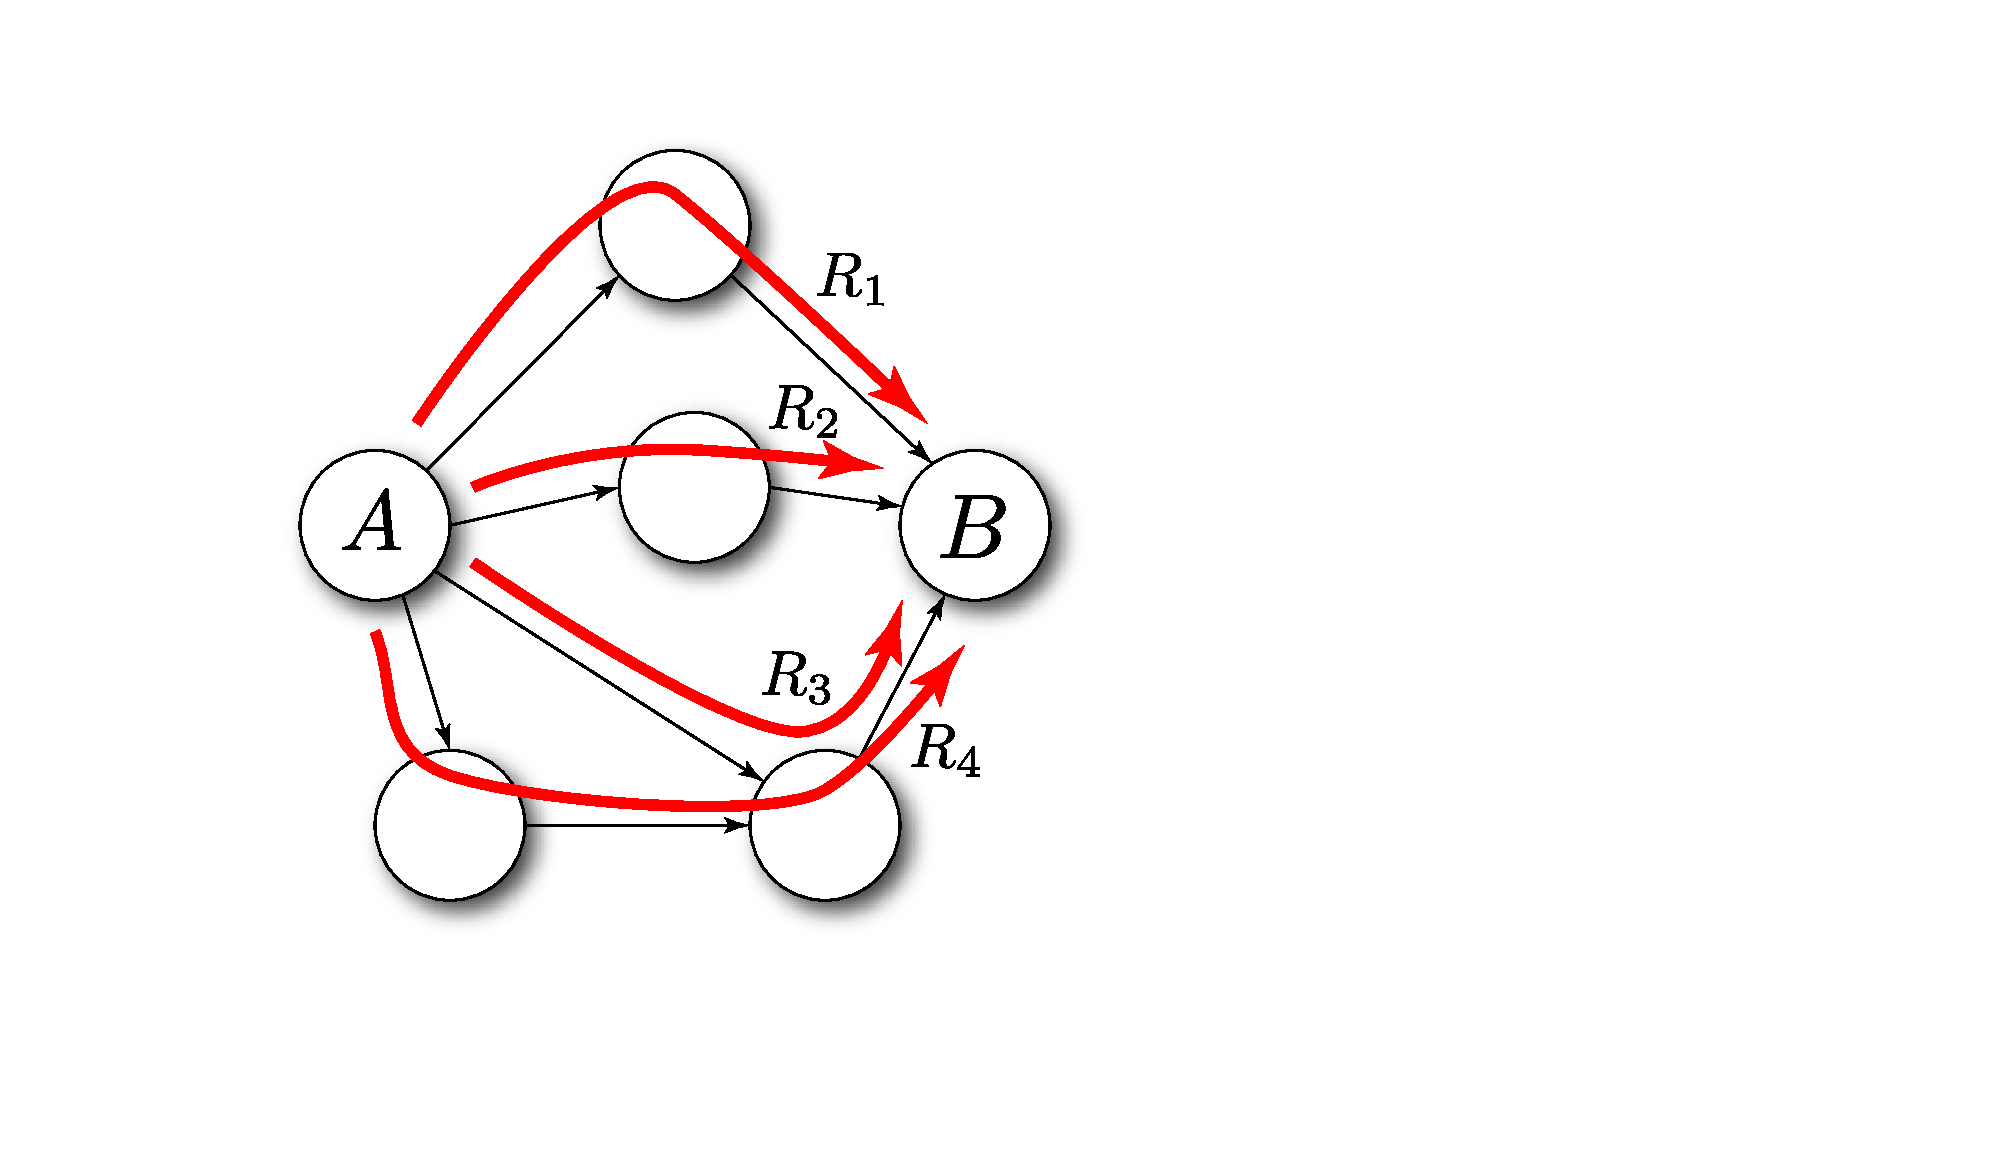
\includegraphics[width=0.65\columnwidth]{example_routes}
\caption{Example of a simple network with multiple routes \mbox{$A\to B$}. Note that $R_3$ and $R_4$ are competing with one another for use of the last link, which the routing strategy, $\mathcal{S}$, will need to resolve if multiple simultaneous transmissions are taking place.} \label{fig:example_routes}
\end{figure}

\begin{figure}[!htb]
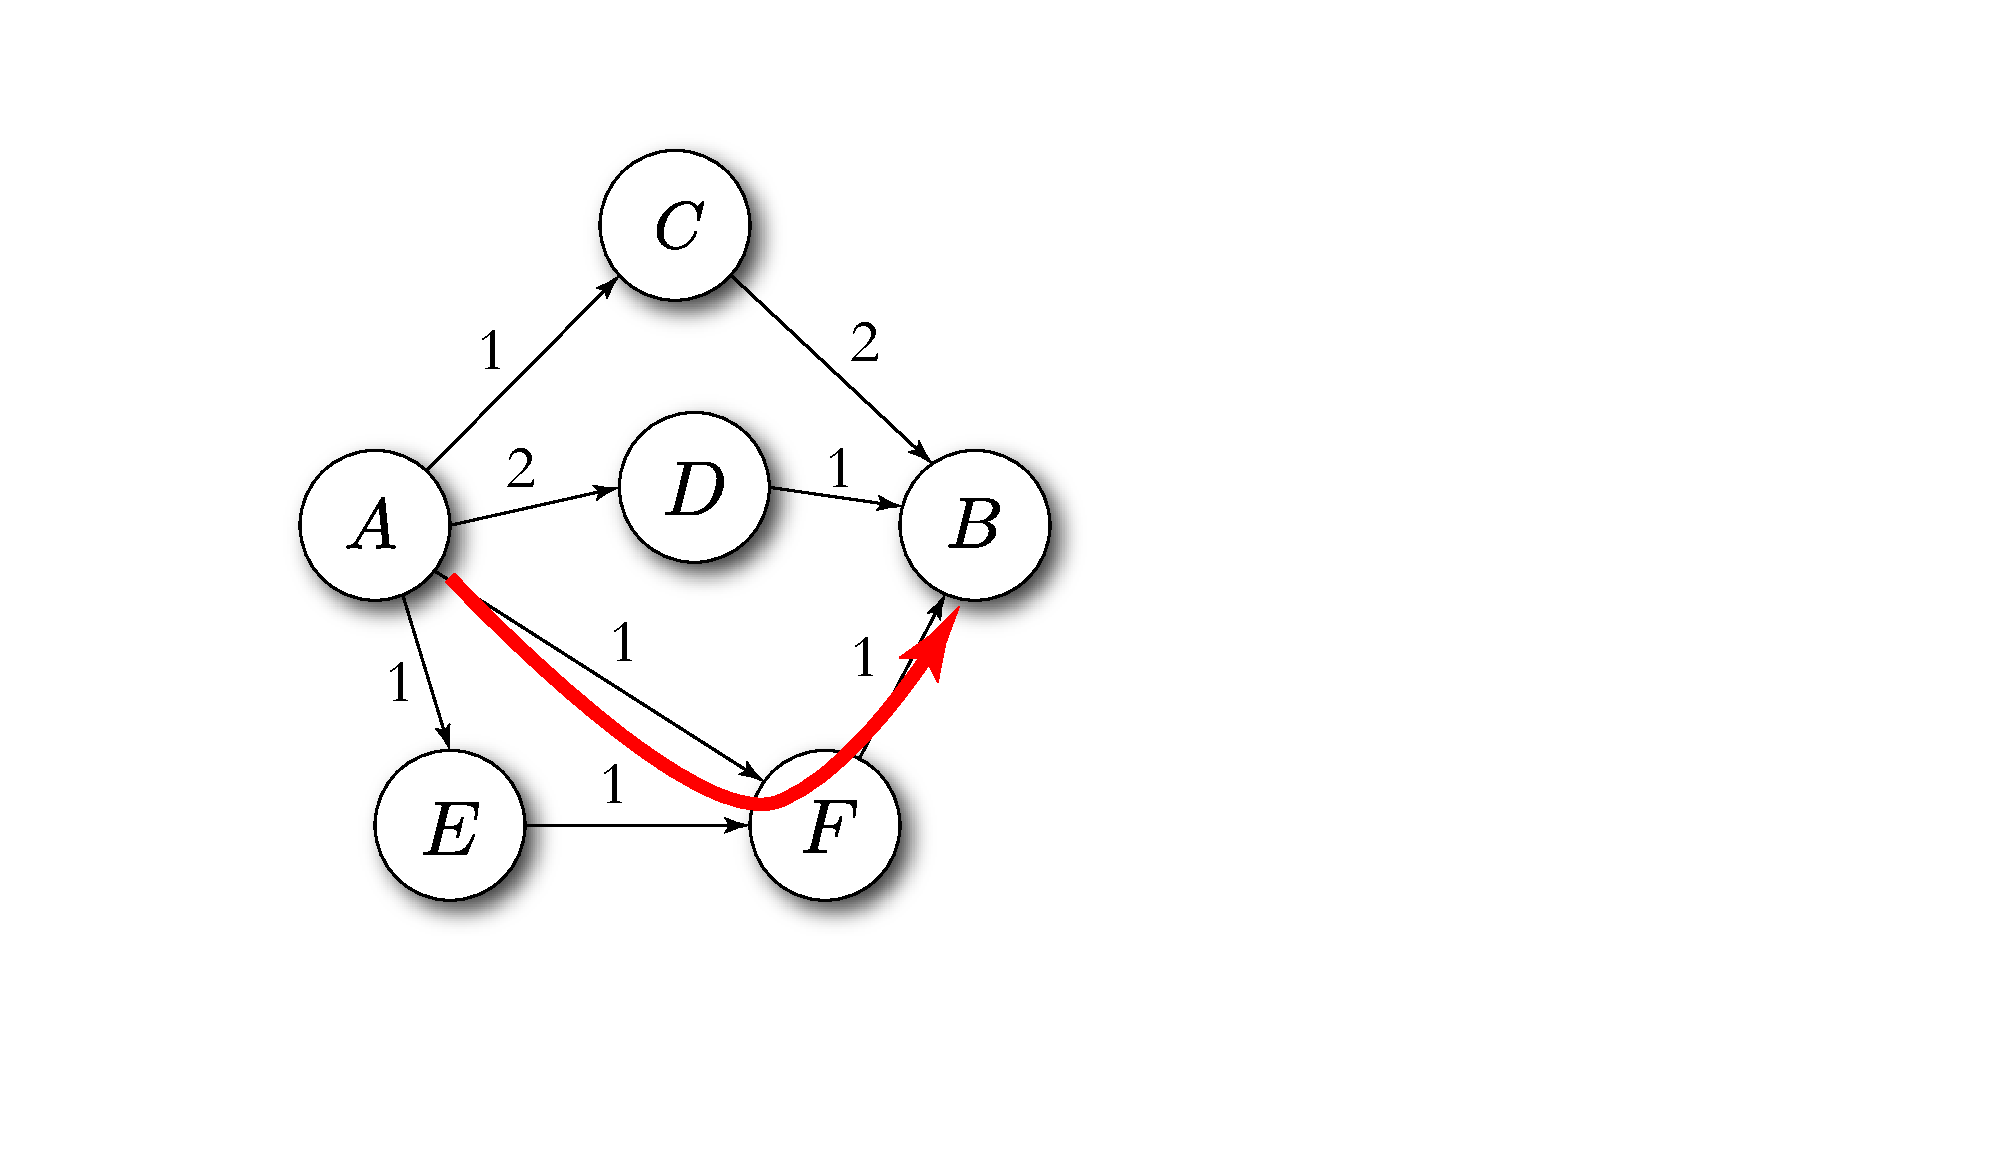
\includegraphics[width=0.6\columnwidth]{example_opt}
\caption{The same network graph from Fig.~\ref{fig:example_routes}, with links weighted by some arbitrary cost metric. Applying a shortest-path algorithm yields the optimal route between Alice and Bob to be \mbox{$A\to F\to B$}, which incurs a net cost of \mbox{$c=2$}, as opposed to all other routes, which incur a net cost of \mbox{$c=3$}.} \label{fig:simp_route_opt}
\end{figure}

In a given network, it is unlikely that only a single cost metric or attribute will be of interest when determining optimal routings. There may be a tradeoff between different measures. For example, for time-critical applications the cost of a route might be considered a combination of both dollar cost and latency -- a satellite has very low latency but is extremely expensive, while a carrier pigeon is slow but cheap. What is the best tradeoff between the two?

To accommodate this, we allow the \emph{net cost} of a route to be defined as an arbitrary function of other primitive cost metrics and attributes of the route,
\begin{align} \label{eq:net_cost_R}
c_\mathrm{net}(R) = f_\mathrm{cost}(\vec{c}(R),\vec{a}(R)),
\end{align}
where $c_\mathrm{net}$ is a single numeric value representing the net cost as calculated from the arbitrary cost function $f_\mathrm{cost}$. Note that the net cost needn't be a metric, as the cost function could be arbitrary. The net cost can be thought of as a ranking for routes, but not necessarily as a metric that accumulates across routes.

Eq.~\ref{eq:net_cost_R} gives us the net cost of a given route. For multiple users we would like to simultaneously optimise the cost across all users of the network. Thus we define the routing cost for the entire network to be,
\begin{align} \label{eq:c_total}
c_\mathrm{total}(\vec{R}_{\vec{A}\to \vec{B}}) = \sum_{r \in {\vec R}_{\vec{A}\to \vec{B}}} c_\mathrm{net}(r),
\end{align}
where $\vec{R}_{\vec{A}\to \vec{B}}$ is a set of routes connecting each pair \mbox{$A_i\to B_i~\forall ~ i$}.

\subsection{Flow Networks} \label{sec:flow_networks}

On a shared network with many users utilising the network simultaneously, it may be the case the preferred goal for the network is to maximise \emph{flow} -- the amount of information that can be transmitted per unit time, i.e the net utilisation of the network's resources. In this case we can build on the existing theory of \emph{flow networks}, which characterise the load of links within the network.

A flow network is easily obtained from the network graph by associating a `capacity' attribute with each link and defining the graph weighted by the capacities as the flow network, preserving the underlying structure of the network graph.

When a route within the graph is utilised, we decrement the capacities of each link in that route, generating the so-called \emph{residual network}, which will now take the place of the original network in subsequent calculations. This process effectively tallies the links' utilisation, and when the tally hits zero, the link can no longer be used for any new routes. This forms a basic building block for more complex flow network algorithms.

There are many variations on flow networks. The simplest case is of a single user transmitting multiple packets simultaneously to a recipient. Depending on link capacities, different packets may need to follow different routes through the network, if network performance is to be maximised. Alternately, it may not be possible to send the desired number packets simultaneously if the network capacity saturates.

The more complex (and realistic) scenario is of multiple users each transmitting from distinct starting nodes to distinct recipient nodes across a shared network. This is known as a \emph{multi-commodity flow network}, and is likely to be the dominant class of networks in real-world networking applications.

\subsection{Routing Strategies} \label{sec:route_strats}

A \emph{strategy}, $\mathcal{S}$, is simply an algorithm that chooses a route ($k$), based on the starting ($i$) and finishing ($j$) nodes of a communication, and also updates the vectors of costs and attributes within the network associated with the utilisation of that route,
\begin{align}
\mathcal{S}(i,j,\vec{c},\vec{a}) &\to \{k,{\vec{c}}~',{\vec{a}}~'\}, \nonumber \\
i,j &\in V, \nonumber\\
k &\in \{R_{v_i\to v_j}\},
\end{align}
with the goal of minimising a chosen cost measure.

No particular route through a network is going to have infinite capacity, and therefore we cannot typically always reemploy the same most cost-effective route for all data. Particularly in multi-user networks, as routes are employed for communicating quantum states, their cost metrics may change according to load, or other external influences. For this reason, it is important that strategies accommodate dynamic changes in the network. This is easily accounted for by letting the edge weights in our network graph be a function of time, $G_t$, which are updated via the application of a strategy, which may also be a function of time,
\begin{align} \label{eq:S_G}
G_{t+1} = \mathcal{S}_t(G_t).
\end{align}
For example, the network might have bandwidth restrictions on some links, in which case if more than a certain amount of data is transmitted through a link, it is no longer available for use until previous transmissions have completed. Or, based on market dynamics, the dollar cost of utilising a link may change with its demand.

\subsection{Strategy Optimisation} \label{sec:strat_opt}

Clearly the goal when choosing routing strategies is to minimize the net cost, Eq.~\ref{eq:net_cost_R}. That is, solving the optimisation problem,
\begin{align}
c_\mathrm{min} &= \min_\mathcal{S} (c_\mathrm{total}), \nonumber \\
\mathcal{S}_\mathrm{opt} &= \mathrm{argmin}_\mathcal{S} (c_\mathrm{total}).
\end{align}

Choosing optimal strategies is a challenging problem, potentially requiring complex, computationally inefficient optimisation techniques. Strategy optimisation is an example of resource allocation, whose optimal solutions are often notoriously difficult to solve, residing in complexity classes like \textbf{NP}-complete (or worse). In general the number of possible routes through a graph will grow exponentially with the number of vertices. Thus, explicitly enumerating each possible route is generally prohibitive for large networks, unless some known structure provides `shortcuts' to optimisation. Having said this, Dijkstra's shortest path algorithm is the perfect counterexample, demonstrating that although an exponential number of routes may exist between two points, an optimal one can be found in polynomial time.

There are two general approaches one might consider when choosing strategies -- \emph{local optimisation} ({\sc Local}) and \emph{global optimisation} ({\sc Global}). {\sc Local} simply takes each state to be communicated, one-by-one, and allows it to individually choose an optimal routing strategy based on the state of the network's costs at that moment. {\sc Global} is far more sophisticated and simultaneously optimises the sum of the routing costs, Eq.~\ref{eq:c_total}, of all currently in-demand routes.

{\sc Global} must clearly perform at least as well as {\sc Local}, since \mbox{{\sc Local}$\subset${\sc Global}}, but we expect it to be better in general owing to the additional information it has of other users on the network. However, {\sc Global} requires solving a complex, simultaneous optimisation problem, which is likely to be computationally hard, whereas {\sc Local} can be efficiently solved using multiple independent applications of, for example, an efficient shortest-path algorithm (so-called `greedy' algorithms).

We will not aim to comprehensively characterise the computational complexity of {\sc Global} strategies. However, in Sec.~\ref{sec:strategies} we will present some elementary analyses of several toy models for realistic strategies. Some such strategies are efficient although not optimal, but nonetheless satisfy certain criteria we might expect.

Future developments in the optimisation techniques required for {\sc Global} strategies may improve network performance, leaving our techniques qualitatively unchanged.

When employing {\sc Local}, on the other hand, things are often far simpler. If we are optimising over a cost metric satisfying the distance interpretation, we may simply employ a shortest-path algorithm to find optimal routes through the network.

If one were to become even more sophisticated, one might even envisage treating network resource allocation in a game theoretic context, which we will not go into here.

\subsection{Message- vs Packet-Level Routing}

In Eq.~\ref{eq:S_G} we defined the action of a strategy, $\mathcal{S}$, on a network, $G$. However, we were intentionally ambiguous in our introduction of the time-dependence, given by $t$. This is to allow us to consider changes at one of two different time-scales: the packet level, or the message level. Recall that the \emph{message} is the entire data stream transmitted from Alice to Bob, whereas the \emph{packet} is a small block of data taken from the message.

When defining the action of strategies, we could do so at either of these time-scales. We could choose routes in their entirety, from start to finish, at the beginning of the message transmission, under the assumption that the costs in the network will be constant over that duration and no one will misbehave. We refer to such strategies as \emph{message-level strategies}. Alternately, and perhaps more realistically in many scenarios, the costs and attributes of a network could be highly dynamic and readily change within the transmission time-window. In that case, we will employ \emph{packet-level strategies}, which reevaluate the strategy independently for each packet and for each of their hops between nodes.

In our future discussions on routing strategies, context will make it clear when we are referring to packet-level or message-level strategies.

\section{Quantum Channels} \label{sec:quant_chan}

Like classical channels, quantum channels are inevitably subject to errors. These errors could be an intrinsic part of the system, or induced by interaction with the external environment. The \emph{quantum process} formalism provides an elegant mathematical description for all physically realistic error mechanisms \cite{bib:Gilchrist05}. Here we review the quantum process formalism and discuss several specific error models that will be of particular interest in quantum networks. This paves the way for the quantum notion of costs and attributes.

\subsection{Quantum Processes}

To quantify the operation of nodes and links within our network, we must characterise the evolution they impose upon quantum states passing through them. Quantum processes, also known as \emph{completely positive maps} (CP-maps) are able to capture all the physical processes relevant to quantum networking, such as: unitary evolution, decoherence, measurement, quantum memory, state preparation, switching, and indeed entire quantum computations.

Quantum processes are able to capture physical processes in any degree of freedom, most commonly in the qubit basis, but also, for photons, in the spatio-temporal, photon-number, or polarisation degrees of freedom.

Quantum processes are most easily represented using \emph{Kraus operators}, $\{\hat{K}_i\}$,
\begin{align}
\mathcal{E}(\hat\rho) = \sum_i \hat{K}_i \hat\rho \hat{K}_i^\dag,
\end{align}
where,
\begin{align}
\sum_i \hat{K}_i^\dag \hat{K}_i = \hat{\mathbb{I}}.
\end{align}
Here $\mathcal{E}$ is a superoperator, denoting the action of the process on state $\hat\rho$. This representation has the elegant interpretation as the probabilistic application of each of the Kraus operators. In the ideal case, the two types of evolution of interest are unitary evolution, in which case there is only one Kraus operator, \mbox{$\hat{K}_1=\hat{U}$}, and projective measurement, where there is again only one Kraus operator, \mbox{$\hat{K}_1=\ket{m}\bra{m}$}, for measurement outcome $m$.

Mathematically, quantum processes are equivalent to a state jointly undergoing unitary evolution with an external environment that is not observed (i.e traced out),
\begin{align}
\mathcal{E}(\hat\rho_S) = \mathrm{tr}_E (\hat{U}_{S,E} [\hat\rho_S\otimes \ket{0}_E\bra{0}_E] \hat{U}^\dag_{S,E}),
\end{align}
where $S$ denotes the primary system to which the process is applied, and $E$ is an auxiliary environment system.

We will require that all our states are normalised,
\begin{align}
\mathrm{tr}(\hat\rho) = 1,
\end{align}
and that our processes are \emph{trace preserving}. That is, they preserve normalisation,
\begin{align}
\mathrm{tr}[\mathcal{E}(\hat\rho)] = 1.
\end{align}

Multiple processes may be composed using the notation,
\begin{align}
\mathcal{E}_n(\dots \mathcal{E}_2(\mathcal{E}_1(\hat\rho)))=(\mathcal{E}_n \circ \dots \circ \mathcal{E}_2\circ\mathcal{E}_1)(\hat\rho).
\end{align}
In general, processes do not commute, i.e \mbox{$\mathcal{E}_1\circ \mathcal{E}_2 \neq \mathcal{E}_2\circ \mathcal{E}_1$}. Unless unitary, quantum processes are irreversible, meaning that errors accumulate and cannot be overcome without the overhead of some form of Quantum Error Correction (QEC).

In general, the Kraus operator representation for quantum processes is not unique -- there may be multiple choices of Kraus operators that implement identical processes. But if the representation is not unique, how do we compare different quantum processes? To address this, it is common to choose a `standard' basis for representing quantum processes, such that they may be consistently and fairly compared. This requires choosing a basis which is complete for operations on the Hilbert space acted upon by the process. For example, for a single qubit, the Pauli operators -- $\sigma_1$ (identity, $\mathbb{\hat{I}}$), $\sigma_2$ (bit-flip, $\hat{X}$), $\sigma_3$ (bit-phase-flip, $\hat{Y}$), and $\sigma_4$ (phase-flip, $\hat{Z}$) -- are complete for single-qubit operations. Therefore by decomposing our Kraus operators into linear combinations of these basis operators we have a standardised representation for single-qubit processes. Formally, for one qubit,
\begin{align}
\mathcal{E}(\hat\rho) = \sum_{i,j=1}^4 \chi_{i,j} \hat{\sigma}_i\hat\rho\,\hat{\sigma}_j^\dag.
\end{align}

The Hermitian matrix $\chi$ is known as the \emph{process matrix}, from which many other metrics of interest may be directly computed (some of which are discussed in Sec.~\ref{sec:quantum_meas_cost}). Process matrices share many properties and interpretations in common with density matrices. The diagonal elements can be regarded as the amplitudes associated with applying each of the four Pauli operators, while the off-diagonal elements represent the coherences between them, i.e whether the operations on the diagonal being applied probabilistically or coherently. For the process to be trace preserving we require,
\begin{align}
\mathrm{tr}(\chi) = 1.
\end{align}

\subsection{Quantum Processes in Quantum Networks} \label{sec:quant_proc_in}

Letting $v_i$ represent the $i$th node within a route $R$, the process associated with communication from that node to the next is $\mathcal{E}_{v_i\to v_{i+1}}$. For the same network used previously, Fig.~\ref{fig:example_proc_graph} shows the quantum processes associated with the links in the network. The cumulative process associated with the entire route is therefore,
\begin{align}
\mathcal{E}_R = \mathcal{E}_{{v_{|R|-1}}\to v_{|R|}} \circ \dots \circ \mathcal{E}_{v_2\to v_3} \circ \mathcal{E}_{v_1\to v_2},
\end{align}
where $|R|$ is the number of nodes in $R$, and to simplify notation, all $v_i$ are implicitly over the route $R$.

\begin{figure}[!htb]
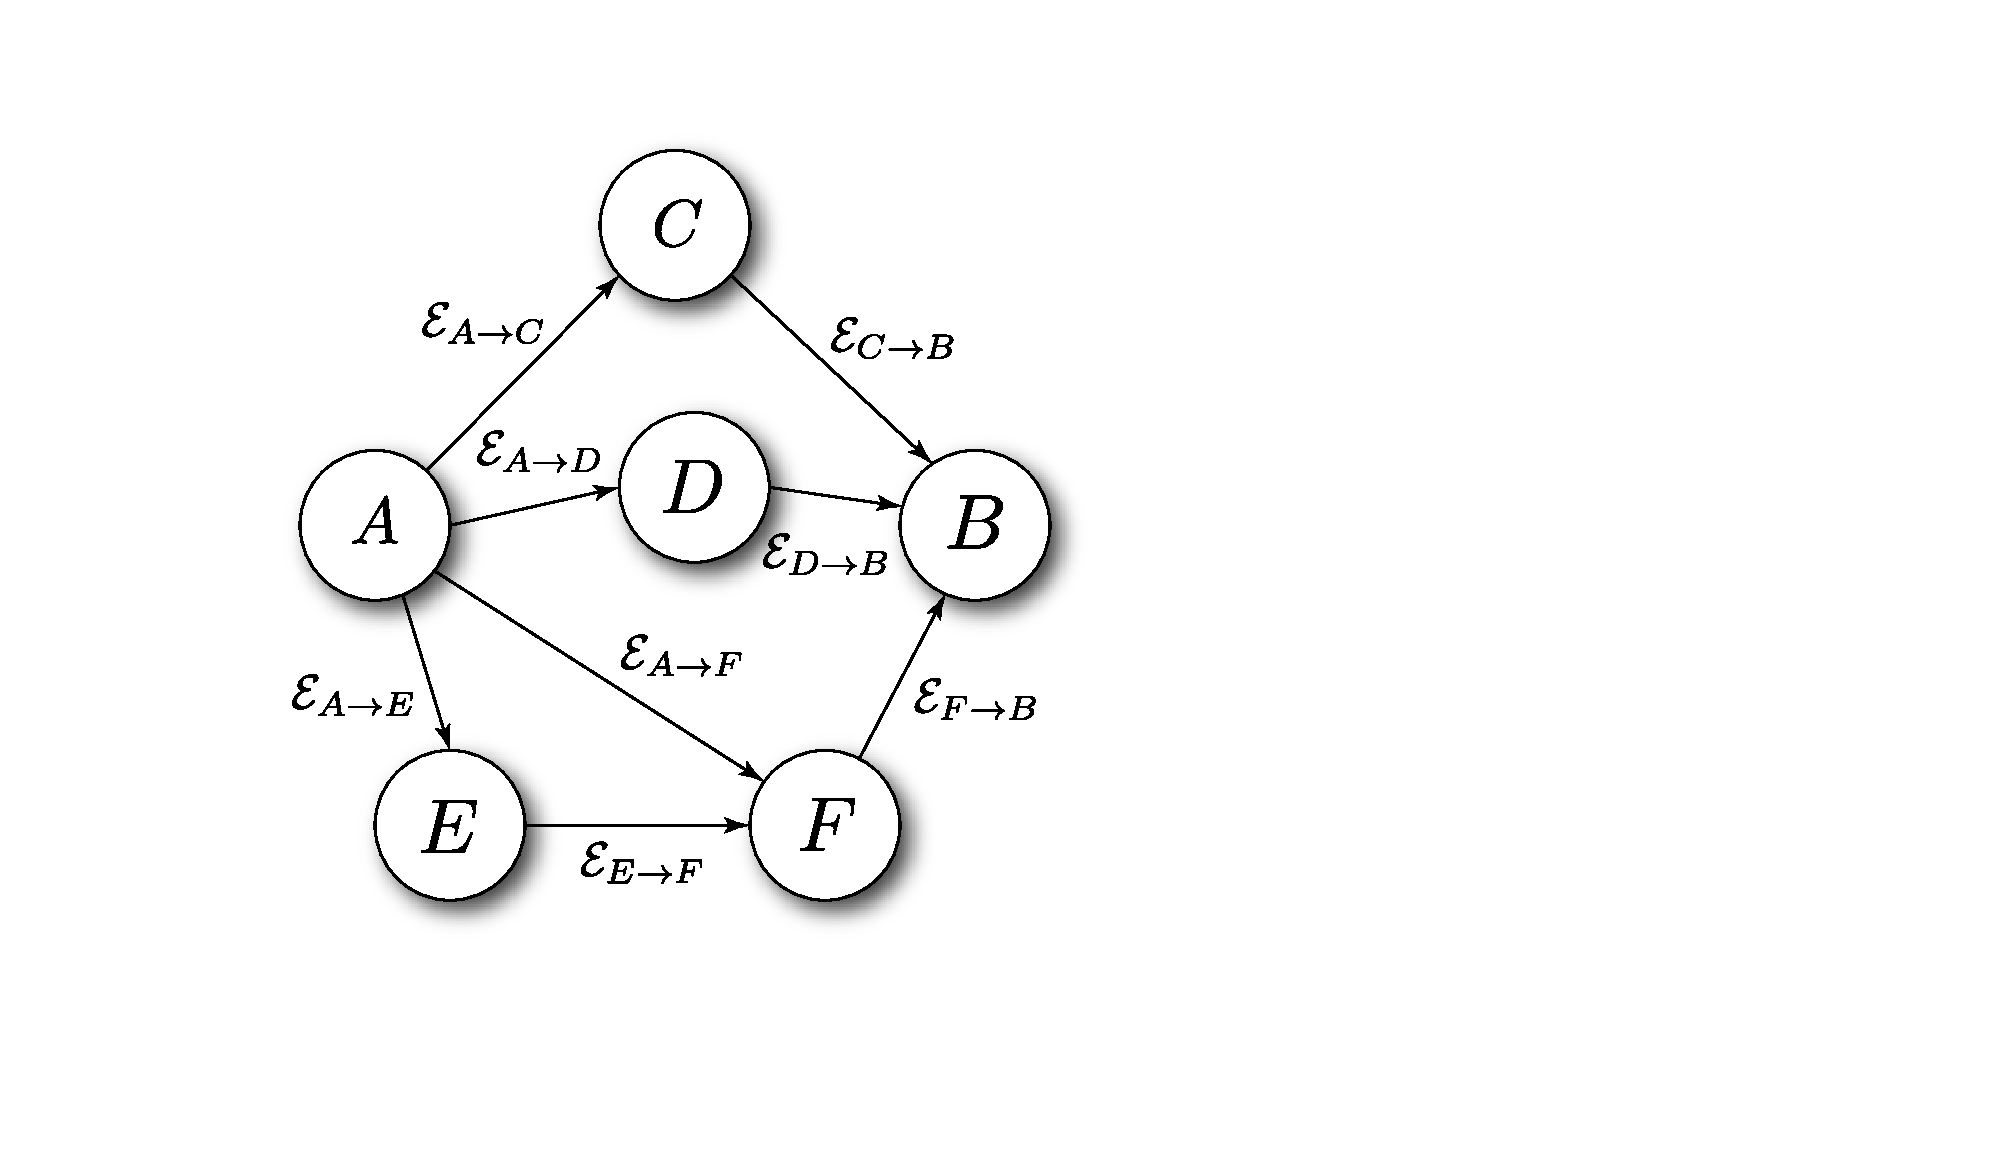
\includegraphics[width=0.6\columnwidth]{example_graph}
\caption{The network from Fig.~\ref{fig:example_routes}, with the quantum processes associated with each link. The net process associated with a route is given by the composition of each of the processes over the length of the route. For example, the route \mbox{$R_1=A\to C\to B$} induces the process \mbox{$\mathcal{E}_{R_1} = \mathcal{E}_{C\to B} \circ \mathcal{E}_{A\to C}$}.} \label{fig:example_proc_graph}
\end{figure}

In general, both nodes and links in a quantum network may implement quantum processes. However, for the purposes of compatibility with the graph-theoretic algorithms employed later, we will eliminate node processes by merging them into link processes, such that the processes in the network are described entirely by links. This reduction procedure is straightforward, shown in Fig.~\ref{fig:remove_nodes}.

\begin{figure}[!htb]
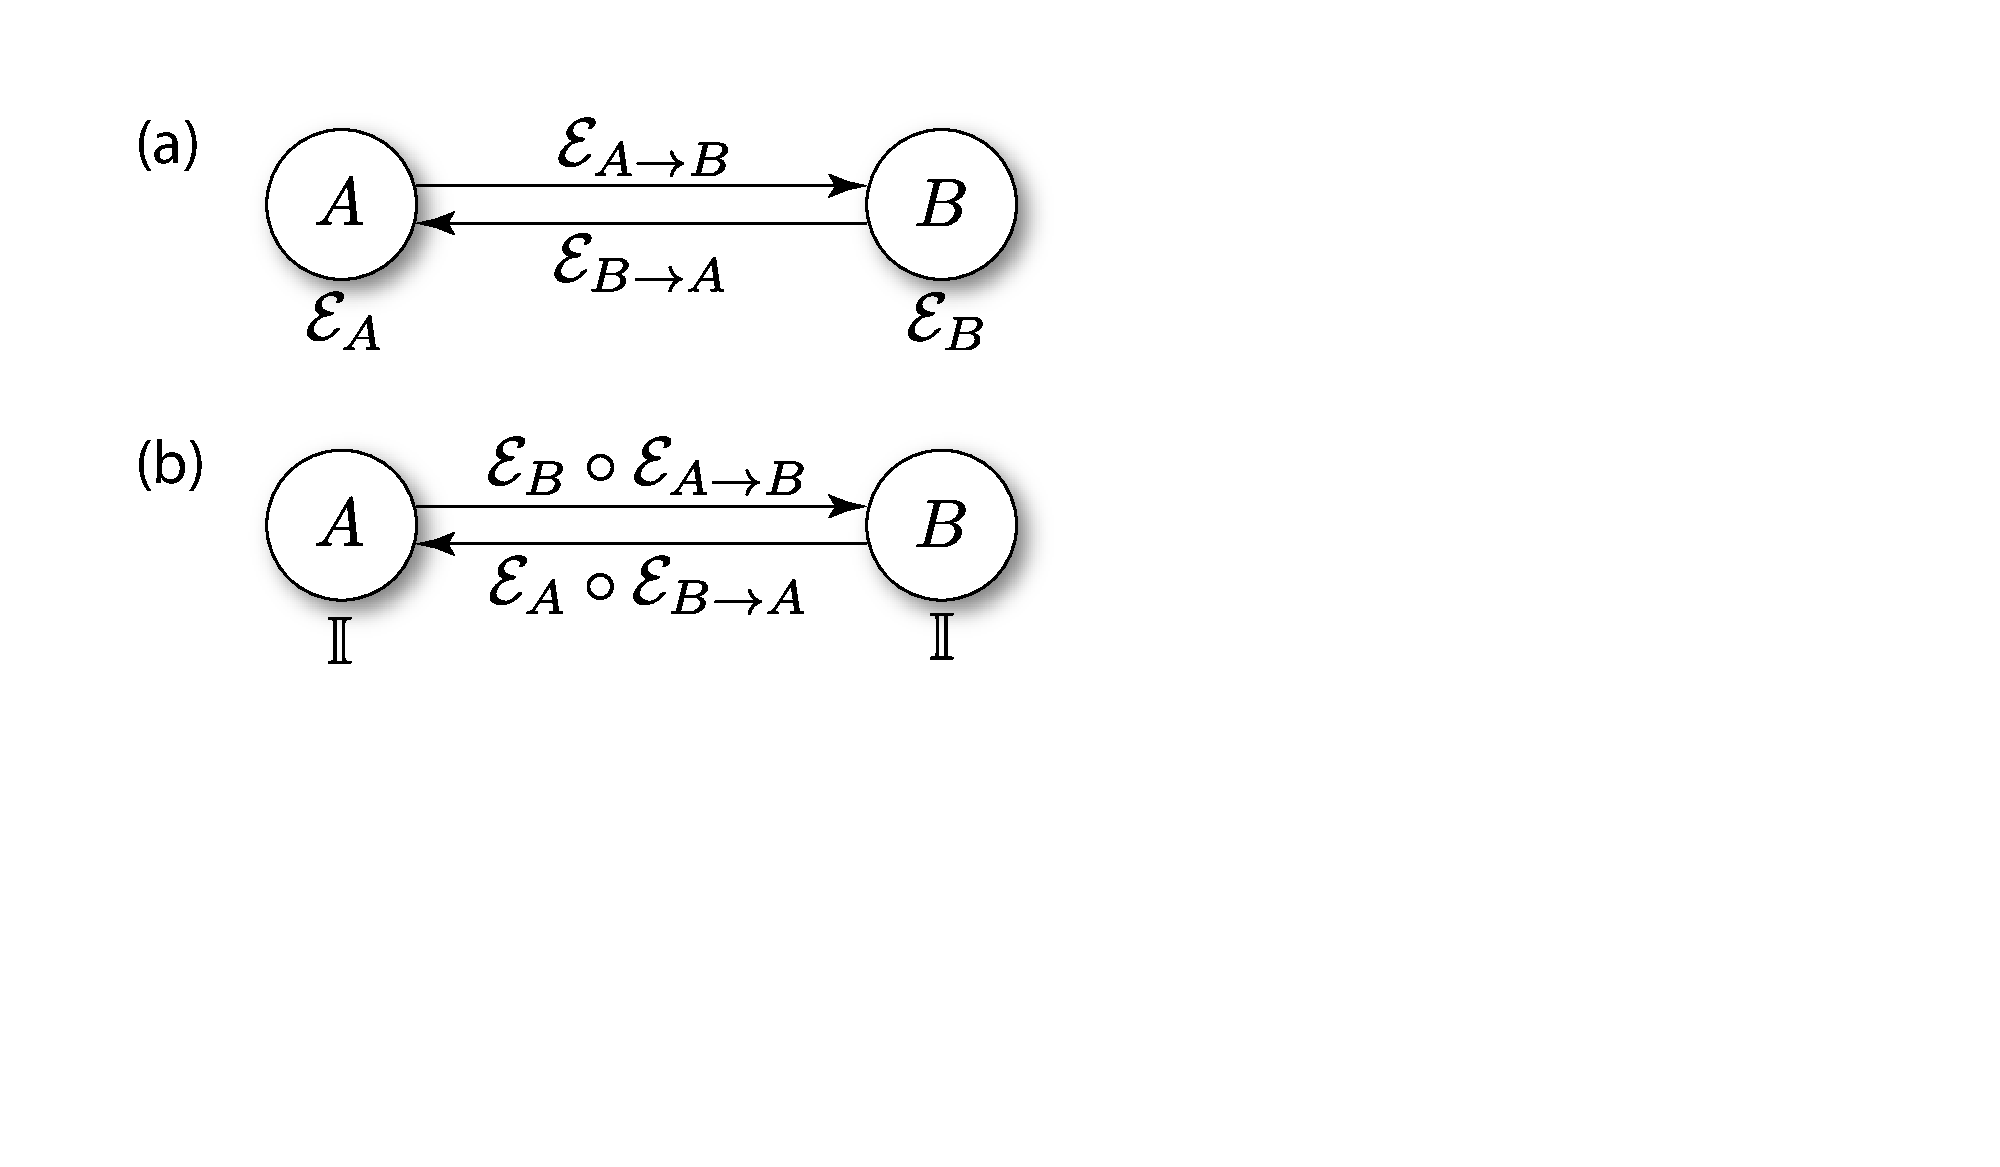
\includegraphics[width=0.7\columnwidth]{remove_nodes}
\caption{Removing node processes from network graphs on a trivial network with two nodes, $A$ and $B$. Each node is associated with a quantum process ($\mathcal{E}_A$ and $\mathcal{E}_B$). Similarly, each link is associated with a process ($\mathcal{E}_{A\to B}$ and $\mathcal{E}_{B\to A}$). (a) Representation where the node and link processes are shown explicitly. (b) The node processes are replaced with identity operations by replacing each link process with the composition of the link process and its target node process. Equivalently, the cost of each node process is added to the cost of \emph{every} incoming link and then eliminated. The same may be applied for attributes rather than costs. This procedure requires that all links be directed. If undirected links are present, they may simply be replaced by two directed links, one in each direction, implementing identical quantum processes each way.} \label{fig:remove_nodes}
\end{figure}

\subsection{Characterising Quantum Channels}

Given a link implementing some arbitrary quantum process, it is essential that it can be experimentally determined such that network performance may be characterised. For example, if an optical channel is lossy, what is the loss rate? This is crucial when attempting to choose routing strategies that optimise certain cost metrics.

Treating a link or node as an unknown black box, \emph{Quantum Process Tomography} (QPT) \cite{bib:ChuangNielsen97} is a technique that may be applied to fully characterise the quantum process it implements, reproducing its complete process matrix. QPT has become a standard procedure, demonstrated in numerous architectures, most notably in optics \cite{bib:OBrien04}. QPT works in general for processes in any degree of freedom, e.g the qubit degree of freedom. However, it is important to note that full QPT requires statistics across the entire basis over which measurements are defined, which typically grows exponentially with the size of the system. For example, the number of measurement bases required to perform full QPT on $n$ qubits grows exponentially with $n$. However, often full process characterisation is not necessary. Instead, knowing particular metrics of interest may suffice. Some of the more noteworthy such metrics will be discussed in Sec.~\ref{sec:quantum_meas_cost}. In this instance, much work has been done in the field of \emph{compressed sensing} \cite{??? compressed_sensing}, in which process metrics of interest can be experimentally determined using far fewer physical resources than via a full reconstruction of the process matrix using QPT.

\section{Optical Encoding of Quantum Information}

While all-optical quantum computing is an unlikely architecture for future scalable quantum computers, it is all but inevitable that optics will play a central role in quantum communications networks. Foremost, this is because photons are `flying' by their very nature and can very easily be transmitted across large distances -- it's quite challenging to transmit a superconducting circuit containing information from Australia to the United States in the blink of an eye! Additionally, optical states are, in many cases, relatively easy to prepare, manipulate and measure, and can also be readily interfaced with other physical quantum systems, allowing the transfer of quantum information from optical communications systems to some other architecture better suited to a given task.

Optical systems are very versatile, allowing quantum information to be optically encoded in a number of ways -- into single photons, many photons, or even an indeterminate number of photons, and in both discrete or continuous degrees of freedom. Different types of encodings may have very different properties in terms of the errors they are susceptible to.

When dealing with single photons, information can be encoded in a number of ways. Most obviously, it can be encoded into the polarisation basis, allowing one bit of information per photon (i.e horizontal and vertical polarisation represent the logical 0 and 1 states). Or it could be directly encoded into the photon-number basis. However, other degrees of freedom, such as the spectral/temporal degrees of freedom could be employed, encoding information into time- or frequency-bins, with potentially far more levels than a simple polarisation qubit \cite{bib:RohdeInfCap13}.

\subsubsection{Single-Photon Qubit Encodings}

A very attractive feature of single photons is that they undergo very little decoherence, even over large distances -- dephasing in the polarisation degree of freedom, for example, is negligible in free-space. They are, however, very susceptible to loss, and protocols relying on many single-photon states suffer exponential decay in their success rates as the number of photons is increased (see Sec.~\ref{sec:eff_err}).

We can encode a single qubit into a single photon in the polarisation basis using the horizontal and vertical polarization degrees of freedom. Equivalently, one can employ `dual rail' encoding, whereby a single photon is placed into a superposition across two spatial modes. This leads to the equivalent representations for qubits,
\begin{align} \label{eq:single_photon_enc}
\ket{\psi}_\mathrm{qubit} &= \alpha\ket{0} + \beta\ket{1}, \nonumber \\
\ket{\psi}_\mathrm{pol} &= \alpha\ket{H} + \beta\ket{V}, \nonumber \\
\ket{\psi}_\mathrm{dual} &= \alpha\ket{0,1} + \beta\ket{1,0}.
\end{align}

\subsubsection{Photon-Number Qudit Encoding}

Of course, the photon-number degree of freedom needn't be limited to 0 or 1. By fully exploiting the photon-number degree of freedom, we can encode a qudit of arbitrary dimension into a single optical mode,
\begin{align} \label{eq:number_qudit}
\ket\psi_\mathrm{qudit} = \sum_{n=0}^\infty \alpha_n \ket{n}.
\end{align}
This may give the impression that a single optical mode has infinite information capacity. Needless to say, this sounds too good to be true, and it is. Loss decoheres photon-number-encoded states exponentially with photon-number. So although in principle we can encode an $\infty$-level qudit, the moment any non-zero loss is introduced, its exponential dependence destroys the state (see Sec.~\ref{sec:eff_err}).

\subsubsection{Spectral Qudit Encoding}

Completely independent of the photon-number degree of freedom, are the spatio-temporal degrees of freedom, which encode the spatial, temporal, and spectral structure of photons. In the temporal domain, for example, we could define the temporal structure of a single photon as,
\begin{align}
\ket\psi_\mathrm{temporal} = \int_{-\infty}^\infty \psi(t) \hat{a}^\dag(t)\,dt\,\ket{0},
\end{align}
where $\hat{a}^\dag(t)$ is the time-specific photonic creation operator, and $\psi(t)$ is the temporal distribution function.

Alternately, we can define \emph{mode operators}, which are mathematically equivalent to creation operators, but create photons with a specific temporal envelope,
\begin{align}
\hat{A}^\dag_\psi &= \int_{-\infty}^\infty \psi(t) \hat{a}^\dag(t)\,dt, \nonumber \\
\ket\psi_\mathrm{temporal} &= \hat{A}^\dag_\psi \ket{0}.
\end{align}
Now by defining an orthonormal basis of temporal distribution functions, $\{\xi_i\}$, such that,
\begin{align}
\bra{0} \hat{A}_{\xi_i} \hat{A}^\dag_{\xi_j}\ket{0} = \delta_{i,j},
\end{align}
we can encode a qudit of arbitrary dimension into the spatio-temporal degrees of freedom,
\begin{align}
\ket\psi_\mathrm{qudit} = \sum_{i=1}^\infty \alpha_i \hat{A}^\dag_{\xi_i} \ket{0}.
\end{align}
Again, however, summing to infinity is somewhat fanciful, given any realistic spatio-temporal error model, such as an imperfect frequency response.

\subsubsection{Continuous Variable (CV) Qudit Encoding} \label{sec:CV_enc}

When encoding information optically, we needn't restrict ourselves to photon-number states. We also have a lot of flexibility to encode information in phase-space using Continuous Variable (CV) states, where phase and amplitude relations encode quantum information.

As a simple example, a coherent state, $\ket\alpha$, is parameterised by a single complex value, $\alpha$, given by a phase and amplitude. By manipulating these parameters, information can be encoded into coherent states. We could, for example, define two coherent states of opposite phase to represent qubit basis states,
\begin{align}
\ket{0} &= \ket{\alpha}, \nonumber \\
\ket{1} &= \ket{-\alpha}.
\end{align}
Note, however, that this representation for qubits is only approximate, since the two basis states are not perfectly orthogonal,
\begin{align}
\langle -\alpha|\alpha \rangle = e^{-2|\alpha|^2},
\end{align}
which is non-zero for any finite $\alpha$, whereas for ideal qubits we require \mbox{$\langle 0|1\rangle = 0$}. However, for large $\alpha$, $\ket{\pm\alpha}$ closely approximate orthogonality.

This representation for qubits using coherent states is easily generalised to qudits by considering coherent states orbiting the origin of phase-space at equal angular intervals of \mbox{$2\pi/d$}, for a $d$-level qudit.

Another type of CV state, which can encode quantum information is superpositions of coherent states (colloquially known as `cat' states), with the encoding,
\begin{align}
\ket{0} &\equiv \frac{1}{\sqrt{2(1+e^{-2|\alpha|^2})}} (\ket{\alpha}+\ket{-\alpha}) \nonumber \\
&= \ket{\mathrm{cat_+(\alpha)}},\nonumber \\
\ket{1} &\equiv \frac{1}{\sqrt{2(1-e^{-2|\alpha|^2})}}(\ket{\alpha}-\ket{-\alpha}) \nonumber \\
&= \ket{\mathrm{cat_-(\alpha)}}.
\end{align}
These two basis states contain strictly even or strictly odd photon-number terms respectively, implying they are always orthogonal,
\begin{align}
\langle\mathrm{cat}_+(\alpha)|\mathrm{cat}_-(\alpha)\rangle = 0 \,\,\forall\,\alpha,
\end{align}
making them directly appropriate for qubit encoding, even for weak coherent amplitudes. Unfortunately, cat states are notoriously difficult to prepare.

\section{Errors in Quantum Networks} \label{sec:errors_in_nets}

As with classical data, quantum data is susceptible to corruption during transmission. However, in addition to all the usual classical error models, quantum information is subject to further uniquely quantum errors. These errors can be represented using the quantum process formalism and fully characterised using QPT. We now briefly discuss several of the dominant errors arising in quantum systems.

\subsection{Examples}

\subsubsection{Known Unitaries}

The most trivial error mechanism is when a unitary channel (e.g an identity channel) actually implements some unitary transformation that is not that which is desired. However, the unitary is constant, not varying from trial to trial, and is known, which can be easily determined using QPT on the channel. For example, an optical fibre might induce a polarisation rotation on transmitted photons, but the fibre isn't changing and neither is the rotation. If consistently implementing the same known unitary then reversing it is straightforward in most architectures.

\subsubsection{Efficiency} \label{sec:eff_err}

Given that quantum communication links will typically be optical, the dominant error mechanism is likely to be loss. We let the efficiency, $\eta$, of an optical quantum process be the probability that a given photon entering the channel leaves the channel in the desired mode, or probability \mbox{$1-\eta$} of being lost. In the case of information encoded into single-photon states, e.g using the polarisation degree of freedom, $\eta$ corresponds exactly to the success probability of the communication.

When implementing protocols employing post-selection upon detecting all photons, the protocol will be non-deterministic, where loss equates to the protocol's success probability. Specifically, with $n$ photons, each with $\eta$ efficiency, the net post-selection success probability of the entire device is $\eta^n$. This implies an exponential number of trials in post-selected protocols. Clearly this exponential scaling is of concern, requiring demanding efficiencies in future large-scale implementations.

Formally, let $\mathcal{E}^\mathrm{loss}_\eta$ be the loss channel with efficiency $\eta$. The channel acting on an initially pure single-photon state, $\ket{1}$, can be modeled as a beamsplitter with transmissivity $\eta$ acting on the state, where the reflected mode is traced out. This yields,
\begin{align}
\mathcal{E}^\mathrm{loss}_\eta(\ket{1}\bra{1}) = (1-\eta)\ket{0}\bra{0} + \eta\ket{1}\bra{1}.
\end{align}
This process would apply equivalently to both horizontal and vertical polarizations. Therefore, via linearity, the loss channel acting on a polarization-encoded qubit (Eq.~\ref{eq:single_photon_enc}) yields,
\begin{align}
\mathcal{E}^\mathrm{loss}_\eta(\ket\psi_\mathrm{pol}\bra\psi_\mathrm{pol}) = (1-\eta) \ket{0}\bra{0} + \eta\ket\psi_\mathrm{pol}\bra\psi_\mathrm{pol}.
\end{align}
The same applies in the context of dual-rail encoding.

In the case of higher order photon-number encoding of qudits, as per Eq.~\ref{eq:number_qudit}, the probability that a state containing terms of at most $n$ photons being maintained scales as $\eta^n$. That is, if the highest photon-number term in our qudit is $n$, that component has an exponentially low probability of being preserved through the loss channel. For this fundamental reason, photon-number encoding does not enable infinite-dimensional qudits to be encoded.

Coherent states are the one example of states, which are in a sense robust against loss, since a lossy coherent state is another coherent state with lower amplitude, but without any loss in coherence,
\begin{align}
\mathcal{E}^\mathrm{loss}_\eta(\ket\alpha\bra\alpha) = \ket{\eta\alpha}\bra{\eta\alpha}.
\end{align}

To the contrary, while cat states are simple superpositions of coherent states, they are extremely sensitive to loss. This is because cat states have well-defined photon-number parity (even or odd), and therefore the loss of just a single photon will flip a cat state to an orthogonal one. Since the probability of photon loss occurring increases exponentially with photon-number, large amplitude cat states are exponentially sensitive to loss channels.

\subsubsection{Dephasing} \label{sec:dephasing_error}

The dephasing error model describes the deterioration of quantum coherence in a state. It does not change the actual amplitudes of the components in the superposition, but rather reduces the state to a mixture of those components. Thus, dephasing can be thought of as destroying quantum information (coherence), while retaining classical information (probability amplitudes). In terms of qubits, dephasing is most commonly represented using the Kraus representation,
\begin{align} \label{eq:dephasing_channel}
\mathcal{E}_p^\mathrm{dephasing}(\hat\rho) = p\cdot\hat\rho + (1-p)\cdot \hat{Z}\hat\rho\hat{Z},
\end{align}
where $\hat\rho$ is the state of a single qubit, and $\hat{Z}$ is the Pauli phase-flip operator. Intuitively this tells us that the dephasing channel creates a mixture of an input state with its phase-flipped self. An alternate interpretation for the dephasing channel is that it is equivalent to the outside environment measuring $\hat\rho$ in the logical ($\hat{Z}$) basis, but unknown to us, thereby projecting the state onto one basis state or another, yielding a mixture of the two. Dephasing acting on $\hat\rho$ can be very elegantly visualised as simply nullifying the off-diagonal matrix elements, i.e eliminating coherence terms. Dephasing is a ubiquitous error mechanism and affects all current quantum computing architectures.

As a simple example, consider the \mbox{$p=1/2$} dephasing channel acting on the \mbox{$\ket{+} = (\ket{0}+\ket{1})/\sqrt{2}$} state. Then we have,
\begin{align}
\mathcal{E}^\mathrm{dephasing}_{1/2}(\ket{+}\bra{+}) &= \frac{1}{2} (\ket{+}\bra{+} + \hat{Z}\ket{+}\bra{+}\hat{Z}) \nonumber \\
&= \frac{1}{2} (\ket{+}\bra{+} + \ket{-}\bra{-}) \nonumber \\
&= \frac{1}{2} (\ket{0}\bra{0} + \ket{1}\bra{1}) \nonumber \\
&= \frac{\mathbb{\hat{I}}}{2},
\end{align}
is the complexity mixed state. That is, the state has completely decohered. Note, however, that this complete decoherence depended on the choice of input state. A computational basis state, on the other hand, would be left unchanged by this channel,
\begin{align}
\mathcal{E}^\mathrm{dephasing}_{1/2}(\ket{0}\bra{0}) &= \frac{1}{2} (\ket{0}\bra{0} + \hat{Z}\ket{0}\bra{0}\hat{Z}) \nonumber \\
&= \ket{0}\bra{0}.
\end{align}

The notion of dephasing can be easily generalised to non-qubit systems. In general, dephasing has the property of mapping a superposition of basis states to a mixture of the same basis states, whilst preserving amplitudes. Thus, for perfect dephasing,
\begin{align}
\mathcal{E}^\mathrm{dephasing}\left(\sum_i \alpha_i\ket{i} \cdot \sum_j \alpha_j^*\bra{j} \right) \to \sum_i |\alpha_i|^2 \ket{i}\bra{i},
\end{align}
for some arbitrary basis enumerated by $i$.

Note that the probability of no dephasing occurring over multiple dephasing channels in series is given by the product of the respective probabilities for the individual channels.

\subsubsection{Depolarisation}

Depolarisation is a noise model more general than dephasing, that probabilistically replaces a state with the completely mixed state (regardless of the input state). That is, with some probability we lose \emph{all} quantum \emph{and} classical information, i.e both coherences and probability amplitudes. Note that the dephasing channel introduced above only destroys quantum coherence, whilst preserving amplitudes. Formally, the depolarising channel can be expressed as,
\begin{align} \label{eq:depolarizing_channel}
\mathcal{E}^\mathrm{depolarizing}_p(\hat\rho) = p \cdot \hat\rho + (1-p)\cdot \frac{\mathbb{\hat{I}}}{\mathrm{dim}(\hat\rho)},
\end{align}
where $\mathbb{\hat{I}}/\mathrm{dim}(\hat\rho)$ is the completely mixed state in the $d$-dimensional Hilbert space.

When acting on qubits, the depolarizing channel can equivalently be represented as the action of each of the four Pauli matrices with equal probability, since,
\begin{align}
\frac{\mathbb{\hat{I}}}{2} = \frac{1}{4}(\hat{I}\hat\rho\hat{I} + \hat{X}\hat\rho\hat{X} + \hat{Y}\hat\rho\hat{Y} + \hat{Z}\hat\rho\hat{Z}).
\end{align}
Thus, both dephasing and depolarization are examples of Pauli error models.

In the qubit basis (i.e not including loss, for example), the Pauli matrices form a complete basis for quantum operations. Thus, the depolarizing channel is the most general qubit error model, since it effectively applies all four Pauli error channels. For this reason, when evaluating fault-tolerance thresholds for QEC codes, thresholds are typically quoted in terms of the depolarizing error rate.

Like the dephasing channel, the error probability of multiple channels in series accumulates multiplicativly.

\subsubsection{Mode-Mismatch} \label{sec:MM_error}

Mode-mismatch is an error model unique to optical implementations. For perfect interference to take place between two optical modes, which is necessary to entangle them, the photons in those modes must be perfectly indistinguishable, i.e they must exhibit identical spatio-temporal structure \cite{bib:RohdeMauererSilberhorn07}. The Hong-Ou-Mandel (HOM) \cite{bib:HOM87} \emph{visibility} is a direct measure of the indistinguishability of two photons based on their interference fringes. Specifically, interference fringes are reduced as the photons become more distinguishable. Once completely distinguishable, they obey classical statistics.

In real-world experiments, the most common form of mode-mismatch is temporal mode-mismatch, whereby the timing of different photons are not perfectly synchronised, yielding temporal distinguishability, and thereby reduced quantum interference. This type of error is easily introduced via mismatched path lengths in an experiment, or incorrectly accounted for changes in refractive index. This is easily represented mathematically via translations in the temporal distribution functions of photons,
\begin{align}
\psi(t) \to \psi(t+\tau),
\end{align}
for temporal mismatch $\tau$.

Mode-mismatch has been studied extensively in the context of linear optics quantum computing (LOQC) \cite{bib:KLM01}. In particular, it was shown that in the cluster state formalism (see Sec.~\ref{sec:CSQC}), mode-mismatch is equivalent to a dephasing error model, where the dephasing rate is related to the degree of photon distinguishability (i.e visibility) \cite{bib:RohdeRalph06}. More generally, the operation of entangling gates \cite{bib:RohdeFreqTemp05, bib:RohdeGateChar05, bib:RohdeOptPhot05, bib:RohdeTimeRes11} and boson-sampling \cite{bib:RohdeArbSpec15, bib:RohdeArbLow12} have been considered, and explicit error models derived.

\section{Quantum Cost Metrics} \label{sec:quantum_meas_cost}

As with the classical case in Sec.~\ref{sec:costs}, there will be costs associated with the links and nodes in a network -- nothing is free! In the quantum case, all the usual classical costs are valid, but there are some very important additions of far greater relevance to most quantum applications. Classical digital data is discretised, resulting in data transmission highly robust against noise. In a quantum setting this is necessarily not the case, as the coefficients in quantum superpositions are not discrete, meaning that errors accumulate during transmission and states will inevitably deteriorate. This requires a rethinking of appropriate cost metrics.

\subsection{Examples} \label{sec:sig_errs}

We now briefly introduce some of the key measures for quantifying the quality of quantum communications links, and how they may be expressed as metrics with meaningful operational interpretations. Many of the measures typically employed for characterising quantum systems are not true metrics (i.e costs), but in many cases can be converted to metrics, or used meaningfully as attributes instead.

\subsubsection{Efficiency}

The efficiency measure introduced previously is multiplicative, so for consecutive lossy channels the net efficiency is,
\begin{align}
\eta_\mathrm{net}=\prod_i \eta_i,
\end{align}
where $\eta_i$ is the efficiency of the $i$th channel. Intuitively, this is simply telling us that if a photon passes through a channel with success probability $\eta_1$, followed by another with $\eta_2$, the total success probability is \mbox{$\eta_1\eta_2$}.

When employing single-photon encoding of qubits (e.g using the polarisation degree of freedom), there are three basis states of interest: a single photon horizontally polarised ($\ket{H}$), a single photon vertically polarised ($\ket{V}$), and the vacuum state ($\ket{\mathrm{vac}}$). The effect of the loss channel on this type of state is to map $\ket{H}$ and $\ket{V}$ to $\ket{\mathrm{vac}}$ with probability \mbox{$1-\eta$}, while doing nothing to $\ket{\mathrm{vac}}$. Note that because the loss process affects both logical basis states ($\ket{H}$ and $\ket{V}$) identically, its action is invariant under unitary operations in the logical (i.e polarisation) basis space.

\subsubsection{Decoherence}

The dephasing and depolarizing channels, given by Eq.~\ref{eq:dephasing_channel} \& Eq.~\ref{eq:depolarizing_channel}, behave multiplicatively. If $p_i$ is the probability that the state passing through the $i$th channel in series does not undergo the error process, then the probability of the state passing though the entire series without error is simply,
\begin{align}
p_\mathrm{net}=\prod_i p_i,
\end{align}
exhibiting the same multiplicative behaviour as the loss channel.

\subsubsection{Fidelity} \label{sec:fid_metric}

The fidelity of two states directly quantifies how close they are to one another in a geometric sense (i.e on the Bloch sphere), or, in the context of a state passing through a quantum channel, a measure of how well the state is preserved.

The fidelity between two states is defined as,
\begin{align}
\mathcal{F}(\hat\rho_1,\hat\rho_2) = \mathrm{tr}\left(\sqrt{\hat\rho_1^{1/2}\cdot\hat\rho_2\cdot\hat\rho_1^{1/2}}\right),
\end{align}
where,
\begin{align}
0\leq \mathcal{F}(\hat\rho_1,\hat\rho_2) \leq 1.
\end{align}
\mbox{$\mathcal{F}(\hat\rho_1,\hat\rho_2)=1$} iff the states are equal, and \mbox{$\mathcal{F}(\hat\rho_1,\hat\rho_2)=0$} iff they are orthogonal.
In the case where one of the states is a pure state, this simplifies to,
\begin{align}
\mathcal{F}(\hat\rho_1,\ket{\psi_2}) = \bra{\psi_2}\hat\rho_1\ket{\psi_2}.
\end{align}

The fidelity is invariant under a common unitary applied to both states,
\begin{align}
\mathcal{F}(\hat\rho_1,\hat\rho_2) = \mathcal{F}(\hat{U}\hat\rho_1 \hat{U}^\dag,\hat{U} \hat\rho_2\hat{U}^\dag).
\end{align}

We define the fidelity of two processes to be the minimum fidelity of two copies of a state passing through the processes, minimised over all possible states. That is, it provides a lower bound on the fidelity of states evolved under the two processes. In the context of networking, where quality must be guaranteed, this definition is more appropriate than say the average case fidelity. Specifically,
\begin{align}
\mathcal{F}(\mathcal{E}_1,\mathcal{E}_2) &= \min_{\hat\rho} \left[\mathcal{F}(\mathcal{E}_1(\hat\rho),\mathcal{E}_2(\hat\rho))\right] \nonumber \\
&= \mathrm{tr}\left(\sqrt{\chi_1^{1/2}\cdot\chi_2\cdot\chi_1^{1/2}}\right),
\end{align}
\comment{CHECK THIS!} where $\chi_1$ and $\chi_2$ are the process matrices for $\mathcal{E}_1$ and $\mathcal{E}_2$.

The fidelity of two processes is invariant under a common unitary applied to both channels before or after the process. Specifically,
\begin{align}
\mathcal{F}(\mathcal{E}_1,\mathcal{E}_2) &= \mathcal{F}(\mathcal{E}_U\circ\mathcal{E}_1,\mathcal{E}_U\circ\mathcal{E}_2) \nonumber \\
&= \mathcal{F}(\mathcal{E}_1\circ \mathcal{E}_U,\mathcal{E}_2\circ \mathcal{E}_U),
\end{align}
where $\mathcal{E}_U$ is an arbitrary unitary process.

In the special case of an identity channel, $\mathbb{I}$, which is of special interest in many communications scenarios, we employ the shorthand,
\begin{align}
\mathcal{F}(\mathcal{E}) = \mathcal{F}(\mathcal{E},\mathbb{I}) = \min_{\hat\rho} \left[\mathcal{F}(\hat\rho,\mathcal{E}(\hat\rho))\right].
\end{align}
By definition \mbox{$\mathcal{F}(\mathcal{E})=1$} iff \mbox{$\mathcal{E}=\mathbb{I}$}.

A lower bound on the process fidelity of multiple processes in series is multiplicative,
\begin{align}
\mathcal{F}(\mathcal{E}_2\circ\mathcal{E}_1,\mathcal{E}_3) &\geq \mathcal{F}(\mathcal{E}_2,\mathcal{E}_3)\cdot\mathcal{F}(\mathcal{E}_1,\mathcal{E}_3), \nonumber \\
\mathcal{F}(\mathcal{E}_2\circ\mathcal{E}_1) &\geq \mathcal{F}(\mathcal{E}_2)\cdot\mathcal{F}(\mathcal{E}_1).
\end{align}

Generalising to a sequence of $n$ processes in series yields,
\begin{align}
\mathcal{F}(\mathcal{E}_n\circ\dots\circ\mathcal{E}_1) \geq \prod_{i=1}^n \mathcal{F}(\mathcal{E}_i).
\end{align}

\subsubsection{Purity}

The purity of a state that was initially pure quantifies how quantum coherence was maintained during evolution, equivalently how well superpositions are maintained. The purity is defined as,
\begin{align}
\mathcal{P}(\hat\rho) = \mathrm{tr}(\hat\rho^2),
\end{align}
where,
\begin{align}
\frac{1}{\mathrm{dim}(\hat\rho)} \leq \mathcal{P}(\hat\rho) \leq 1.
\end{align}
We have \mbox{$\mathcal{P}(\hat\rho) = 1$} iff \mbox{$\hat\rho=\ket{\psi}$} is a pure state, and \mbox{$\mathcal{P}(\hat\rho)=1/\mathrm{dim}(\hat\rho)$} iff \mbox{$\hat\rho=\mathbb{\hat{I}}/\mathrm{dim}(\hat\rho)$} is the maximally mixed state.

The purity is invariant under unitary operations,
\begin{align}
\mathcal{P}(\hat\rho) = \mathcal{P}(\hat{U}\hat\rho\,\hat{U}^\dag).
\end{align}

The purity of a process is defined analogously to the fidelity of a process (but only minimising over pure states),
\begin{align}
\mathcal{P}(\mathcal{E}) &= \min_{\ket\psi} \left[\mathcal{P}(\mathcal{E}(\ket\psi))\right] \nonumber \\
&= \mathrm{tr}(\chi^2),
\end{align}
\comment{CHECK THIS!} and as with the fidelity, a lower bound on the purity of multiple processes in series is multiplicative,
\begin{align}
\mathcal{P}(\mathcal{E}_2\circ\mathcal{E}_1)
\geq \mathcal{P}(\mathcal{E}_2)\cdot\mathcal{P}(\mathcal{E}_1).
\end{align}
If the channel implements a unitary operation then necessarily \mbox{$\mathcal{P}(\mathcal{E})=1$}.

Like the process fidelity, the purity of a quantum process is invariant under unitary operations,
\begin{align}
\mathcal{P}(\mathcal{E}) &= \mathcal{P}(\mathcal{E}_U\circ\mathcal{E}) \nonumber \\
&= \mathcal{P}(\mathcal{E}\circ\mathcal{E}_U).
\end{align}

Generalising to a sequence of $n$ processes in series yields,
\begin{align}
\mathcal{P}(\mathcal{E}_n\circ\dots\circ\mathcal{E}_1) \geq \prod_{i=1}^n \mathcal{P}(\mathcal{E}_i).
\end{align}

\subsubsection{Entanglement} \label{sec:ent_meas}

When distributing entanglement between separate nodes, metrics quantifying bipartite entanglement are relevant. For pure bipartite states $\ket{\psi}_{A,B}$, the purity of one of the reduced subsystems directly quantifies the degree of entanglement between them,
\begin{align}
\mathcal{M}(\ket{\psi}_{A,B})) &= \mathcal{P}(\mathrm{tr}_A(\ket{\psi}_{A,B})) \nonumber \\
&= \mathcal{P}(\mathrm{tr}_B(\ket{\psi}_{A,B})),
\end{align}
The entanglement between two systems in invariant under local unitaries,
\begin{align}
\mathcal{M}(\ket{\psi}_{A,B}) = \mathcal{M}([\hat{U}_A\otimes \hat{U}_B]\ket{\psi}_{A,B}).
\end{align}
\comment{What about for processes?}

\subsubsection{Channel Capacity}

The measures considered until now have quantified the preservation of quantum states. Alternately, one might consider information theoretic measures, which quantify the number of bits/qubits transmitted by a link, i.e the number of bits/qubits in common before and after the link's quantum process. This is an extremely powerful tool as it upper bounds the amount of information the receiver can extract from the transmitter under \emph{any} measurement scheme, very useful in a cryptographic context.

The Shannon entropy of a classical probability distribution $X$ is given by,
\begin{align}
H(X) = -\sum_x p_x\mathrm{log}_2(p_x),
\end{align}
or for a joint distribution over $X$ and $Y$,
\begin{align}
H(X,Y) =  -\sum_{x,y} p_{x,y}\mathrm{log}_2(p_{x,y})
\end{align}

The von Neuman entropy for quantum density operators, $S(\hat\rho)$, is defined analogously, replacing probabilities with density operator eigenvalues,
\begin{align}
S(\hat\rho) &= - \sum_x \lambda_x \mathrm{log}_2 (\lambda_x) \nonumber \\
&= -\mathrm{tr}(\hat\rho\,\mathrm{log}\,\hat\rho),
\end{align}
where $\lambda$ are the eigenvalues of $\hat\rho$. This modification is logically justified, as the eigenvalues can be interpreted directly as a purely classical probability distribution of orthogonal states when the density operator is transformed into a basis with no coherences between basis states (i.e a diagonal basis or spectral decomposition). In that case the Shannon and von Neuman entropies essentially have identical physical interpretations.

The \emph{mutual information} specifies the number of bits in common between two distributions. Equivalently, it is the maximum number of bits that one party can learn about the other. For two classical distributions, $A$ and $B$, this is given by,
\begin{align}
I(A;B) = H(A) + H(B) - H(A,B).
\end{align}

Equivalently, for density operators,
\begin{align}
I(\hat\rho_A;\hat\rho_B) = S(\hat\rho_A) + S(\hat\rho_B) - S(\hat\rho_A,\hat\rho_B),
\end{align}
The mutual information between two quantum states is invariant under local unitary transformations,
\begin{align}
I(\hat\rho_A;\hat\rho_B) = I(\hat{U}_A\hat\rho_A \hat{U}_A^\dag; \hat{U}_B\hat\rho_B \hat{U}_B^\dag),
\end{align}
\comment{CHECK THIS!} since the eigenvalue spectrum of a density operator is invariant under unitary transformation. Therefore, the mutual information represents the maximum amount of information Bob can learn about Alice's state under \emph{any} local operations.

The mutual information is defined as being between a particular known pair of states. Of course, in a quantum network we will seldom know what the states being communicated are and will therefore be unable to directly calculate the mutual information. To address this, the \emph{classical channel capacity} of a channel is defined as,
\begin{align}
\mathcal{C}(\mathcal{E}) = \max_{\hat\rho} I(\hat\rho,\mathcal{E}(\hat\rho)),
\end{align}
with the intuitive interpretation as the maximum mutual information between input and output states that can be achieved for the channel. (Note: this definition of `capacity' is not to be confused with that which we referred to in flow networks).

Analogous to the mutual information for classical systems is the \emph{coherent information} for quantum systems \cite{???}. The coherent information quantifies the number of qubits \comment{Check this!} (as opposed to bits) in common, before and after a channel, defined as,
\begin{align}
I(\hat\rho,\mathcal{E}) = S(\mathcal{E}(\hat\rho)) - S_e(\hat\rho,\mathcal{E}).
\end{align}
Here $S_e$ is the \emph{exchange entropy}, a measure of how much information is exchanged between the state $\hat\rho$ and the environment under the action of the process. This yields the intuitive interpretation that the coherent information is the information contained in the evolved state, discounted by the amount lost to the environment.

The quantum coherent information exhibits much of the same mathematical structure as the classical mutual information. And analogously, we can define the \emph{quantum channel capacity} as,
\begin{align}
\mathcal{Q}(\mathcal{E}) = \max_{\hat\rho} I(\hat\rho,\mathcal{E}).
\end{align}

Analytic solutions to $\mathcal{C}(\mathcal{E})$ and $\mathcal{Q}(\mathcal{E})$ are not known even for simple Pauli error channels such as dephasing and depolarization. However, once net dephasing or depolarization rates have been calculated across a route, the channel capacities can easily be solved numerically, which is sufficient for the numerical algorithms we will rely upon.

\subsubsection{Latency} \label{sec:latency_metric}

Aside from the actual information content of a transmitted quantum state, the latency associated with its transmission is a key consideration in many time-critical applications.

By defining the latency of a link/node as the time between receipt of a quantum state and its retransmission, the total latency of a route is simply the sum of all the individual node and link latencies across the route,
\begin{align}
\mathcal{L}(R) = \sum_{i\in R} \mathcal{L}_i,
\end{align}
where $\mathcal{L}_i$ is the latency associated with the $i$th link in route $R$.

\subsubsection{Dollars} \label{sec:dollars}

Not to be overlooked is the actual dollar cost of communicating information. It is unlikely that Alice and Bob outright own the entire infrastructure of particular routes. Rather, different links and nodes are likely to be owned by different operators (particularly in ad hoc networks), who are most likely going to charge users for bandwidth in their network (quantum networks won't be cheap). Clearly dollar costs are additive over the links and nodes within routes,
\begin{align}
\mathcal{C}(R) = \sum_{i\in R} \mathcal{C}_i,
\end{align}
where $\mathcal{C}_i$ is the dollar cost of utilising the $i$th link in route $R$.

\subsection{Costs as Distance Metrics} \label{sec:cost_as_dist}

Def.~\ref{def:metric} defines the properties of a cost metric in the classical context. We now wish to consider this in the quantum context.

If we consider a lossy photonic channel for example, efficiencies ($\eta$) are multiplicative. For a route \mbox{$v_1\to v_2\to v_3$}, the net efficiency is given by the product of the individual efficiencies, \begin{align}
\eta_{v_1\to v_3} = \eta_{v_1\to v_2} \eta_{v_2\to v_3}.
\end{align}
This is multiplicative rather than additive, clearly not satisfying our definition for a cost metric. However, multiplicative metrics such as this can easily be made additive by shifting to a logarithmic scale, since
\begin{align}
\log(\eta_{v_1\to v_3}) = \log(\eta_{v_1\to v_2}) + \log(\eta_{v_2\to v_3}),
\end{align}
which now has a legitimate interpretation as a distance. In general, for a series of links \mbox{$v_1\to v_2 \to \dots \to v_n$} characterised by multiplicative measure $m$, the equivalent cost metric is,
\begin{align} \label{eq:dist_log}
c_{v_1\to v_2 \to \dots \to v_n} = -\sum_{i=1}^{n-1} \mathrm{log}(m_{v_i\to v_{i+1}}).
\end{align}
We have assumed that \mbox{$0\leq m \leq 1$}, where \mbox{$m=0$} represents complete failure, and \mbox{$m=1$} represents ideal operation.

With these properties, the costs in our graph have an elegant interpretation. In the case of perfect operation, \mbox{$m=1$}, the cost is \mbox{$c=0$}, creating an ideal direct link between neighbouring nodes at no cost. On the other hand for complete failure, \mbox{$m=0$}, the cost metric is \mbox{$c=\infty$}, effectively removing the link from the network and prohibiting pathfinding algorithms from following that route altogether.

Such a logarithmic scale is particularly convenient when a cost metric over links accumulates on a per physical distance basis, in which case the cost metric is simply the physical length of the link times the metric per unit distance. For example, if a fibre channel implements loss at 3dB/km, then the loss over 10km is 10$\times$3dB.

Note that lower bounds on fidelity, purity, efficiency and dephasing are all multiplicative on a scale of 0 to 1, and thus their logarithms may be regarded as cost metrics.

Latency and dollar cost are clearly metrics as they are additive.

In the case of mutual information, which is not a metric, one can use it to define the \emph{variation of information} metric,
\begin{align}
d_\mathrm{VI}(X,Y) &= H(X,Y) - I(X;Y), \nonumber \\
d_\mathrm{VI}(\hat\rho_A,\hat\rho_B) &= S(\hat\rho_A,\hat\rho_B) - I(\hat\rho_A;\hat\rho_B),
\end{align}
or for a channel,
\begin{align}
d_\mathrm{VI}(\hat\rho,\mathcal{E}) &= S(\hat\rho,\mathcal{E}(\hat\rho)) - I(\hat\rho;\mathcal{E}(\hat\rho)),
\end{align}

\subsection{Non-Trivial Node Operations}

Thus far we have considered how to accumulate cost metrics across routes through a network, where each link is subject to some quantum process obeying our notion of a cost metric. But what happens when the links are interspersed with nodes that may be doing more than just simple switching?

A more general scenario to consider is where the nodes are not restricted to routing, but can additionally implement arbitrary unitary operations. This substantially broadens the class of networks under consideration, to encompass nodes capable of doing everything from straightforward routing to entire quantum computations.

All of the examples for cost metrics we introduced in Sec.~\ref{sec:quantum_meas_cost} have the property that they are invariant under unitary operations. Therefore the costs along a route may simply be accumulated as before, summing up the edge weights, without needing any special treatment for node operations, provided they are unitary. For non-unitary node processes, we can merge them into their neighbouring link processes as before (see Fig.~\ref{fig:remove_nodes}).

\section{Quantum Networks} \label{sec:quant_net}

Quantum networks comprise all the same ingredients as classical networks, but with additions. Nodes can additionally implement quantum computations, quantum-to-classical interfaces (i.e measurements), quantum-to-quantum interfaces (interconnects), quantum memories, or any quantum process in general. The cost associated with links could include measures that are uniquely quantum, such as fidelity, purity or entanglement measures, none of which are applicable to classical digital data. As in the classical case, our goal is to find routing strategies that optimise a chosen cost metric. But in the quantum context costs will be constructed entirely differently owing to the quantum nature of the information being communicated.

We envisage a network with a set of senders, $\{A_i\}$, and receivers, $\{B_i\}$, residing on a time-dependent network graph $G_t$ as before. $A$ have sets of quantum states to communicate, $\{\hat\rho_\mathrm{data}(i)\}$. For each $\hat\rho_\mathrm{data}(i)$ she must choose appropriate strategies $S_t$, such that the overall cost is optimised, for some appropriate cost measure. Compared to classical resources, equivalent quantum resources are costly and must be used efficiently, making resource allocation strategies of utmost importance.

The routing strategies we introduce in Sec.~\ref{sec:strategies} will not always guarantee that packets have immediate access to network bandwidth the moment they demand it. Inevitably, in shared networks there will sometimes be competition, forcing some users to wait their turn. For this reason, many quantum networks will require at least some nodes (the ones liable to competition) to have access to quantum memories, such that quantum packets can be stored for a sufficient duration that they can wait their turn on the shared network resources. Of course, quantum memories induce quantum processes of their own, which need to be factored into cost calculations. Quantum memories are easily accommodated for in the QTCP framework by allowing self-loops at nodes, which implement a memory process. The implementation of quantum memory is discussed in Sec.~\ref{sec:memory}.

Given that classical networking is decades more advanced than quantum networking, and extremely cheap and reliable, we will assume that classical resources `come for free', and only quantum resources are of practical interest. That is, classical communication and computation is a free resource available to mediate the operation of the quantum network. We therefore envisage a \emph{dual network} with two complementary networks operating in parallel and in tandem -- the quantum network for communicating quantum data, and a topologically identical classical network operating side-by-side and synchronised with the quantum network.

\section{The Quantum Transmission Control Protocol (QTCP)}

In the classical world, TCP is employed for data transmission and routing. Next we define the quantum equivalent -- the Quantum Transmission Control Protocol (QTCP).

There have been numerous approaches employed in the past for sharing communications links between multiple users. This includes channel-switched networks, time- or frequency-multiplexed networks, and Code Division Multiple Access (CDMA). Nowadays packet-switched networks have become the norm in most digital networks, as they facilitate far greater efficiency in the use of network bandwidth, and are more easily scaled to greater numbers of users in a dynamic and ad hoc manner. It is foreseeable the same trend will continue with quantum technologies, especially given their initial high cost, where maximising network utility is paramount.

The goal of QTCP is to abstract away the low-level physical operation of a quantum network to create a virtual interface between Alice and Bob, allowing direct access to data as if it were held locally, in much the same way that high-level services like the File Transfer Protocol (FTP) facilitate interaction with remote data as though it were a local asset, blind to the intermediate networking.

We consider the scenario where Alice (or a set of Alice's) has some state, which she wishes to communicate to Bob (Bob's), with the aim of optimising some arbitrary cost measure. Bob is no guru and doesn't want to concern himself with how the state got from Alice to himself. His only concern is that he receives it and that it satisfies quality constraints he and Alice have agreed upon.

QTCP is the joint software/hardware stack that facilitates these objectives. QTCP begins by logically separating different levels of network functionality into distinct layers in a protocol stack. The stack is described in detail in Sec.~\ref{sec:prot_stack}. In addition to simple packet switching, the protocol stack is responsible for two very important problems -- routing \emph{strategies} (to be discussed in Sec.~\ref{sec:strategies}), and \emph{collision detection} (Sec.~\ref{sec:collision}). Both of these problems are very low-level in nature, and must be abstracted away by QTCP such that the end user is oblivious to their operation.

\section{QTCP Protocol Stack} \label{sec:prot_stack}

As with classical networking, our protocols for quantum networks will be separated into distinct layers, each performing a specific set of tasks with different levels of abstraction.

The structure of the protocol stack for QTCP is shown in Fig.~\ref{fig:stack}. In summary, the layers in the protocol stack are, beginning from the lowest level:
\begin{itemize}
\item {\sc Data (Message)}: Raw data Alice wishes to transmit to Bob. Comprises both {\sc Quantum Data} and {\sc Classical Data}.
\item {\sc Packet}: Decomposition of {\sc Data} into blocks ({\sc Packet Data}), and associated classical {\sc Packet Headers} containing metadata (e.g routing information).
\item {\sc Strategy}: Construct {\sc Packet} routing strategies based on a cost optimisation algorithm.
\item {\sc Transport}: Physical routing of {\sc Packets} to arrive at their destination, based upon metadata contained in {\sc Packet Header}. Perform collision detection during transit.
\item {\sc Reconstruction}: Reconstruct {\sc Data} from received {\sc Packets}.
\item {\sc Quality of Service (QoS)}: Apply QEC and determine whether {\sc QoS} requirements have been satisfied.
\item {\sc Services \& Applications}: High-level interface to {\sc Data} presented to Bob's services and applications. The interface abstracts away lower levels of the protocol stack, presenting Bob with only {\sc Data} and its associated metadata.
\end{itemize}

\begin{figure}[!htb]
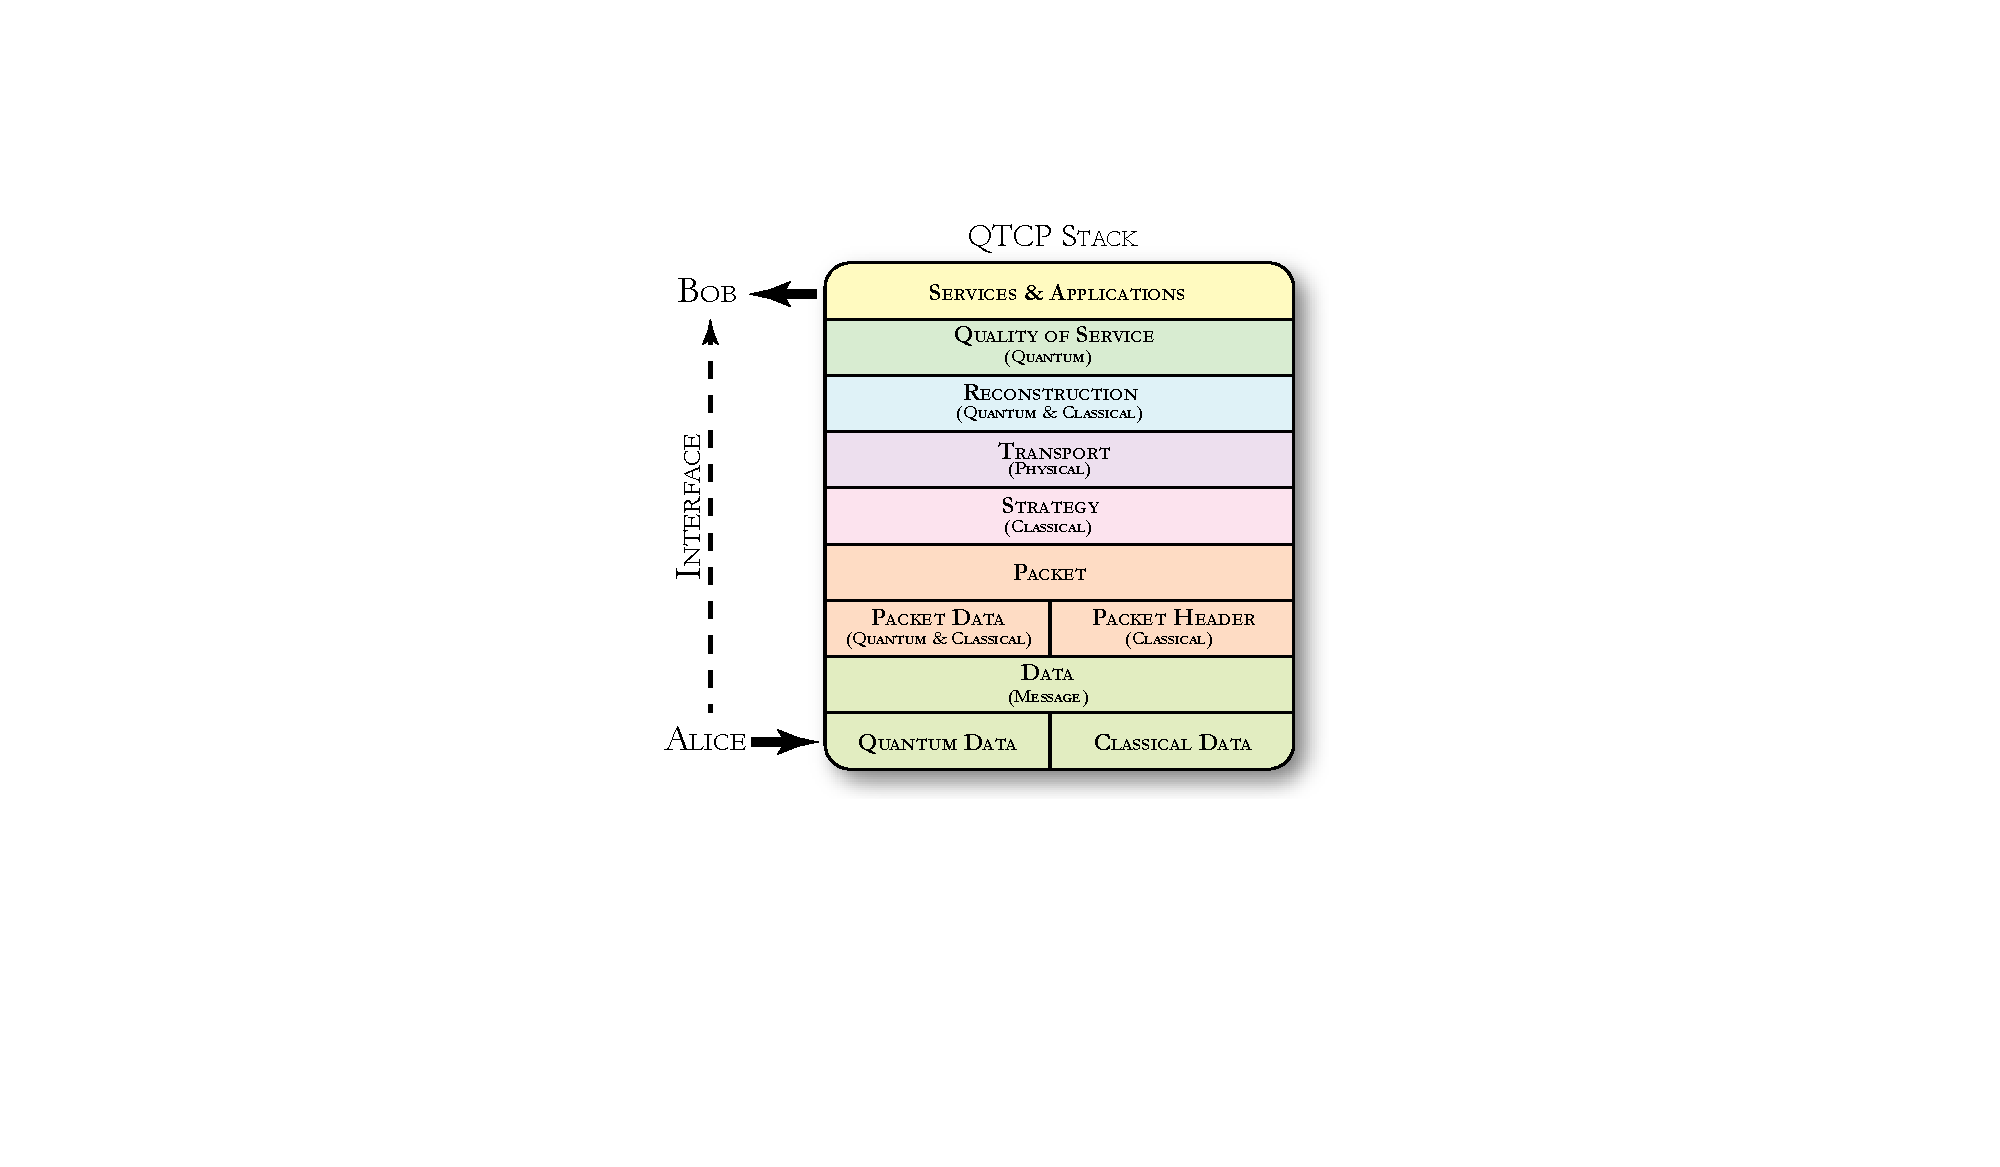
\includegraphics[width=\columnwidth]{stack}
\caption{Protocol stack for QTCP. The protocol stack mediates communication of quantum data from Alice to Bob using the shown layers of abstraction. The end goal is to provide Bob a virtual interface to Alice's transmitted data, while remaining oblivious to the underlying protocol.} \label{fig:stack}
\end{figure}

Next we describe the operation of the layers in the protocol stack in detail.

\subsection{Data (Message)}

At the lowest level of the protocol we have the raw {\sc Data} Alice wishes to communicate to Bob. {\sc Data} is allowed to comprise both {\sc Quantum Data} and {\sc Classical Data} components, and may contain one or the other, or both.

\subsubsection{Quantum Data}

{\sc Quantum Data} is allowed to be an arbitrary quantum state. It could be a pure or mixed state, of arbitrary (but predetermined) dimension, or even a subsystem of a larger external state (i.e entangled with another system).

\subsubsection{Classical Data}

{\sc Classical Data} is a purely classical state with no coherence (i.e a diagonal density matrix), which may be represented as a classical bit-string. We very intentionally segregate the {\sc Classical} and {\sc Quantum} components of {\sc Data}, since the classical network is expected to be cheaper and more reliable than the quantum network operating in parallel to it. The {\sc Classical Data} could, for example, provide nodes with classical instructions on what quantum computations to perform on the {\sc Quantum Data}.

\subsection{Packet}

{\sc Data} is transmitted as {\sc Packets}, much in the same way as conventional TCP. The {\sc Data} is decomposed into three components: {\sc Quantum Data}, {\sc Classical Data}, and {\sc Packet Header}.

We can express the state of an entire {\sc Packet} as,
\begin{align}
\hat\rho_\mathrm{packet}(i) = \hat\rho_\mathrm{quantum}(i) \oplus \hat\rho_\mathrm{classical}(i) \oplus \hat\rho_\mathrm{header}(i),
\end{align}
where $i$ denotes the $i$th packet. Here $\hat\rho_\mathrm{quantum}$ ($\hat\rho_\mathrm{classical}$) is a block of {\sc Quantum Block Size} qubits ({\sc Classical Block Size} bits) taken from the user's {\sc Quantum Data} ({\sc Classical Data}), while $\hat\rho_\mathrm{header}$ is the {\sc Packet's} classical {\sc Packet Header}. As discussed earlier, since $\hat\rho_\mathrm{quantum}$ is quantum, and $\hat\rho_\mathrm{classical}$ and $\hat\rho_\mathrm{header}$ are classical, they needn't be transmitted together over the same quantum network. Instead all {\sc Classical Data} and {\sc Packet Header} could be transmitted over a classical network operating in parallel to and synchronised with the quantum network, which carries the {\sc Quantum Data}.

Note that while one can always measure classical data without disturbance, this is not the case with quantum data, where measurements cause wavefunction collapse. Thus, while Alice is always able to know $\hat\rho_\mathrm{classical}$ and $\hat\rho_\mathrm{header}$, she may or may not know $\hat\rho_\mathrm{quantum}$. Clearly if she prepared the state herself, she would (hopefully) know what she was doing. But in general, quantum networks could be used for far less trivial networking, where Alice is, for example, an intermediary in a distributed quantum computation. In this instance, Alice is unlikely to know what her {\sc Quantum Data} is.

\subsubsection{Packet Data}

Comprises blocks of both {\sc Quantum Data} and {\sc Classical Data}, of sizes {\sc Quantum Block Size} and {\sc Classical Block Size} respectively. {\sc Packet Data} requires that {\sc Data} be decomposed into distinct subsystems which are independently transmitted by QTCP. We will restrict ourselves to the case where the {\sc Data} is encoded into a stream of qubits ({\sc Quantum Data}) and bits ({\sc Classical Data}). There is no loss of generality in applying this constraint since any quantum (classical) information can be encoded into qubits (bits), and once represented as such, the decomposition of {\sc Data} into {\sc Packets} arises very naturally and intuitively. The {\sc Packet's} {\sc Quantum Data} is what is transmitted via the quantum channels, while the {\sc Classical Data} is communicated via classical channels.

\subsubsection{Packet Header} \label{sec:packet_header}

{\sc Packet Header} is purely classical and needn't be transmitted over the costly quantum network, instead being transmitted over a complementary classical network, running in parallel to, and synchronised with the quantum network. {\sc Packet Header} contains no information content from {\sc Data}, instead comprising only metadata relevant to the higher levels of the protocol stack. In particular, {\sc Packet Header} contains the following fields:
\begin{itemize}
    \item {\sc Header Size}: The number of bits in the {\sc Packet Header}.
    \item {\sc Message ID}: A unique identifier for the complete message to which this {\sc Packet} belongs. This field mitigates ambiguity as to which {\sc Message} this packet belongs when performing {\sc Reconstruction}.
    \item {\sc Lifetime}: How long the {\sc Packet} has been in existence for, i.e since it was initially sent by the {\sc Sender}. This is used by strategies to prevent collisions.
    \item {\sc Sender}: A unique node identifier for the sender (Alice).
    \item {\sc Recipient}: A unique node identifier for the recipient (Bob).
    \item {\sc Order}: To which block taken from {\sc Data} does this {\sc Packet Data} belong? This is extremely important in networks where {\sc Packets} may arrive out of order. The {\sc Order} field forms the basis for the {\sc Reconstruction} layer.
    \item {\sc Quantum Block Size}: The number of qubits contained in the {\sc Quantum} component of {\sc Packet Data}. This is important for the {\sc Reconstruction} layer.
    \item {\sc Classical Block Size}: The number of bits contained in the {\sc Classical} component of {\sc Packet Data}, also important for the {\sc Reconstruction} layer.
    \item {\sc Routing Queue}: A first in, first out (FIFO) queue of node identifiers, tracing out the entire route for the {\sc Packet} to follow, in chronological order from the next node to visit all the way to the {\sc Recipient}.
    \item {\sc Costs}: A tuple characterising all the accumulated costs of the {\sc Packet} at the current stage in the route. These are treated as accumulators that are incremented appropriately after each step, since costs are additive.
    \item {\sc Attributes}: A tuple characterising all the non-{\sc Cost} properties associated with the {\sc Packet}. Examples include: the {\sc Priority} of routing a {\sc Packet} to its destination; suggesting a preferred routing {\sc Strategy}; or, indicating whether or not a {\sc Resend Until Success} protocol may be applied to this {\sc Packet}.
    \item {\sc Padding}: Null data to pad the joint {\sc Classical Packet Data} and {\sc Packet Header} fields to be of the same length as the {\sc Quantum Packet Data}. This ensures that the components of the {\sc Packet} traversing the quantum and classical channels remain in perfect tandem -- bit for qubit. In Sec.~\ref{sec:transport} we show that this facilitates collision detection without the need to measure quantum states.
    \item {\sc Checksum}: A regular checksum of the entire {\sc Classical} component of the {\sc Packet}, including both {\sc Classical Packet Data} and {\sc Packet Header}. This also forms a part of the collision detection protocol.
\end{itemize}

One might question why {\sc Packet Headers} tally accumulated costs when we ought to already know all the costs, since these were employed by the algorithm for choosing strategies in the first case. In the ideal case where all strategies are determined \emph{a priori} and are implemented as intended, this is certainly valid. However, for generality we retain this option since more realistic networks may require dynamically updating strategies during the course of propagation, in which case dynamically tallying costs is appropriate.

\subsection{Strategy} \label{sec:into_strat}

Based on the {\sc Packet Headers} of all users sharing the network, choose routing strategies to optimise cost metrics. The notion of strategies is introduced in Sec.~\ref{sec:strat_opt}, and a detailed discussion of example strategies is presented in Sec.~\ref{sec:strategies}.

Once routings have been determined for all {\sc Packets}, the {\sc Routing Queues} in their {\sc Packet Headers} are initialised accordingly by pushing the sequence of node identifiers tracing out the desired route.

In the case of dynamic, time-dependent strategies, which can be updated within the duration of transmissions, the {\sc Routing Queues} may need to be updated. A change in a {\sc Packet's} route simply requires flushing the queue and pushing new node identifiers for each of the nodes in the new route, in chronological order.

The {\sc Strategy} layer is responsible for evaluating the net cost function $f_\mathrm{cost}$ from Eq.~\ref{eq:net_cost_R}, which accounts for both {\sc Costs} and {\sc Attributes} to calculate a single effective cost measure that may be employed in routing decisions.

\subsection{Transport} \label{sec:transport}

The {\sc Transport} layer is responsible for actual routing at the physical level, making direct decisions as to what to do with a {\sc Packet} at each step, based upon the metadata contained in {\sc Packet Header}, most notably the {\sc Routing Queue}, which specifies the full route a {\sc Packet} is destined to follow. It is also responsible for keeping track of costs that accumulate over their route.

Additionally, the {\sc Transport} layer is responsible for collision detection, whereby multiple packets being transmitted simultaneously over a network interfere with one another, corrupting the data. In classical networking, collision detection is straightforward using checksums. But the usual classical approach breaks down in the quantum setting. In Sec.~\ref{sec:collision} we discuss in detail collision detection in QTCP.

The pseudo-code algorithm implemented by the {\sc Transport} layer, including collision detection, is shown in Alg.~\ref{tab:transport_alg}.

\begin{table}[!htb]
\fbox{\parbox{0.965\columnwidth}{\tt
function Transport(Packet):
\begin{enumerate}
    \item nextNode = Packet.RoutingQueue.Pop()
    \item Packet.PhysicallySendTo(nextNode)
    \item Packet.WaitUntilArrivesAt(nextNode)
    \item checksum = Hash(Packet.Header + Packet.ClassicalData)
    \item if(checksum $\neq$ Packet.Header.Checksum) \{
    \setlength{\itemindent}{0.2in}
    \item Packet.Sender.Notify({\sc Failure})
    \item Packet.Recipient.Notify({\sc Failure})
    \item Packet.Discard()
    \item $\Box$
        \setlength{\itemindent}{0in}
\item \}
    \item Packet.Costs += IncomingLink.Costs
    \item Packet.Attributes.Update()
    \item if(Packet.RoutingQueue.Length = 0) \{
    \setlength{\itemindent}{0.2in}
    \item Return(Packet)
        \setlength{\itemindent}{0in}
    \item \}
    \setlength{\itemindent}{0in}
    \item $\Box$
\end{enumerate}}}
\caption{Algorithm implemented by the {\sc Transport} layer of QTCP for each {\sc Packet}. The {\tt Attributes.Update()} function is left undefined. This is where arbitrary {\sc Attribute} dynamics may take place.} \label{tab:transport_alg}
\end{table}

\subsection{Reconstruction}

The {\sc Reconstruction} layer only serves one purpose -- to chronologically reorder the received {\sc Packets} based on the {\sc Order} field in their {\sc Packet Headers}. This stage is only performed by Bob -- the final recipient -- and not at any intermediate stage. In general this will require Bob to have a quantum memory, able to hold all {\sc Packet Data} for a sufficient duration as to enable an arbitrary permutation to be applied, reproducing the correct chronological order.

\begin{table}[!htb]
\fbox{\parbox{0.965\columnwidth}{\tt
function Reconstruction(Packets):
\begin{enumerate}
    \item Packets.WaitUntilAllReceived()
    \item message = Packets.SortByOrderAscending().data
    \item Packets.Receiver.Notify(message)
     \item $\Box$
\end{enumerate}}}
\caption{The goal of the {\sc Reconstruction} layer, is to take a collection of received {\sc Packets} and reassemble them into a single data-stream.} \label{tab:reconstruction}
\end{table}

\subsection{Quality of Service (QoS)}

In classical networking theory, error detection is an important element of networking protocols. Communication links may be unreliable, or subject to external noise, which users must be able to detect so as to guarantee the quality of their data.

Classically, error detection is typically performed using checksums (hash functions), which generate a short digest of a packet's data that can be recalculated upon arrival to verify integrity. The checksum can be included in the header component of each packet, allowing the remainder of the protocol to remain unchanged.

In the quantum context the elegant notion of checksums is complicated by the fact that calculating a hash function of a quantum state would necessarily entangle the state with the hash function. This would have the undesired effect of causing measurement of the checksum to collapse the quantum state of the data, thereby altering it in an uncontrollable way.

As an alternative to checksums, we could borrow the notion of fault-tolerance from quantum computing theory. Here we encode a quantum state into a (polynomially) larger Hilbert space. \emph{Syndrome measurements} on some of the states in this larger space allow us to both detect and correct universal error models, such as depolarisation or dephasing, provided that error rates are within the fault-tolerance threshold of the code being employed.

Different error correcting codes have different error correcting power, and different resource overheads, which must be taken into consideration. The appropriate choice of code will largely be determined by the final {\sc Services \& Applications} layer. For some simple quantum communications protocols, simple error correction (or even no error correction) may suffice. A full-fledged quantum computation on the other hand will require error rates within a fault-tolerance thresholds.

The field of fault-tolerance is already extremely well developed and could be applied directly to QTCP as an abstraction layer directly below the {\sc Services \& Application} layer of the protocol stack, abstracting it away from the end user.

\begin{table}[!htb]
\fbox{\parbox{0.965\columnwidth}{\tt
function QoS(Packets):
\begin{enumerate}
    \item qec = Packets.ApplyQEC()
    \item if(qec.success = true) \{
    \setlength{\itemindent}{0.2in}
    \item message.Receiver.Notify(qec.data)
    \setlength{\itemindent}{0in}
    \item \} else \{
    \setlength{\itemindent}{0.2in}
    \item message.Receiver.Notify({\sc Failure})
    \setlength{\itemindent}{0in}
    \item \}
    \item $\Box$
\end{enumerate}}}
\caption{QoS algorithm based on any appropriate existing QEC code.} \label{tab:qos}
\end{table}

\subsection{Services \& Applications}

Having communicated all the {\sc Packet Data} from Alice to Bob, performed {\sc Reconstruction}, and applied {\sc QoS} protocols, Bob ought to have $\hat\rho_\mathrm{data}$ to a good approximation. The quality of Bob's received state can be inferred directly from the {\sc Costs} vector contained in the {\sc Packet Headers}. The final state and its associated quality metrics ({\sc Costs} and QEC outcomes) may then be provided to Bob as a software interface for end use.

\section{Collision Handling \& Classical Errors} \label{sec:collision}

In classical networking, protocols such as Ethernet allow users to simply broadcast data at their leisure and rely on \emph{collision detection} to detect when the broadcasts of multiple users have interfered, signalling that both users ought to retransmit after a brief random waiting period (known as `backoff') to minimise the chances of another collision occurring. While this {\sc Resend Until Success} approach has certainly proven to be effective in classical networking, in a quantum setting the rules of the game are entirely different.

First, collision detection necessarily requires measuring a communications channel to test whether data has been corrupted. Classical networks typically do this by transmitting a checksum with the data, which is recalculated upon arrival for comparison. This raises the obvious problem that quantum measurements are destructive, which means that testing the integrity of our data destroys it in the process -- the last feature we'd like our network to exhibit! However, to overcome this, in Sec.~\ref{sec:transport} we describe a protocol based on the dual classical/quantum network that allows collision detection without measuring quantum states.

Second, collision detection is not always even allowed at all. If one of Alice's packets was entangled with another (i.e she was communicating an entangled system, where the different subsystems resided in different packets), she would not be able to simply retransmit an identical copy of the corrupted packet, since the entanglement with the other system would have been lost and there are no local operations she can do to recover it.

Alternately, Alice might be a part of a distributed computation, where she didn't prepare the data in the first place. In this instance, the no-cloning theorem implies that she cannot, in general, learn what the quantum state was, and therefore would be unable to make a second transmission attempt.

From Alice's point of view, {\sc Resend Until Success} would clearly work if she was preparing a known separable state. However, collisions on the network caused by her reckless resending would likely corrupt the communications between other parties, leaving them rather ticked off at her.

There are therefore two main approaches to dealing with collisions. First, central planning of all routing could be employed, precisely scheduling all routes \emph{a priori} so as to entirely eliminate any possibility for collisions. Second, if all users in the network were communicating data where packet loss could be tolerated, they could all mutually agree to use the {\sc Resend Until Success} protocol. This would not require a central authority, and be highly desirable for ad hoc networks. It is important to stress, however, that the latter requires unanimity amongst network participants to function, and the restriction to known, separable states is a major limitation that would prohibit many important uses for quantum networks, such as distributed quantum computation. However, both these approaches are entirely valid in their appropriate context.

In classical TCP all components of data packets are classical and are kept together throughout every stage of transmission. In the quantum case we will instead have a mixture of both quantum and classical data. As mentioned, we will assume that classical communication and computation resources `come for free' (or are at least cheap compared to quantum resources), so there will be a clear disambiguation as to what data is quantum or classical within packets.

As discussed, quantum collision detection is complicated by the fact that measuring quantum data to determine whether it has been corrupted disturbs the quantum state. We address this problem by taking advantage of the duality of the quantum/classical network, discussed in Sec.~\ref{sec:quant_net}. Because the quantum and classical components of the {\sc Packets} are synchronised and of equal length (thanks to the {\sc Padding} field of the {\sc Packet Header}), and because the same applies to all other {\sc Packets} on the network, a collision in the quantum data necessarily implies a collision in the classical data, and vice versa. Therefore, by applying regular classical collision detection techniques based on checksums (recall {\sc Packet Header} has a {\sc Checksum} field), we can infer collisions in quantum data without actually measuring it. We refer to this as \emph{indirect collision detection}. This guarantees us the ability to detect when a collision has occurred, in which case both quantum \emph{and} classical data are corrupted, or has not occurred, in which case both quantum and classical data are uncorrupted and the quantum data remains unmeasured. Collision detection is incorporated into the pseudo-code implementation of the {\sc Transport} layer shown in Alg.~\ref{tab:transport_alg}.

This algorithm could, depending upon implementation, be executed locally on the node currently hosting the {\sc Packet}, or it could be delegated to a central authority, but with the overhead of additional classical communication.

In instances where corruption or loss of packets cannot be tolerated, a more proactive approach may be applied. To preempt the risk of packet collision, one could introduce \emph{probe packets} -- packets containing only classical data, that query a route ahead to negotiate channel usage for the following proper packet, thereby avoiding collisions. Of course, if an upcoming node is unable to guarantee channel capacity immediately, the packet may need to be stored in quantum memory until the channel is available. Thus, it is important to accommodate for this by ensuring that quantum memory is available in nodes preceding links/nodes where collisions are not guaranteed to be mitigated immediately. Quantum memory will be discussed in Sec.~\ref{sec:memory}.

\section{Strategies} \label{sec:strategies}

In Sec.~\ref{sec:costs} we introduced the notion of network costs, strategies for allocating network resources in Sec.~\ref{sec:route_strats}, and a general formalism for optimising strategies so as to minimise costs in Sec.~\ref{sec:strat_opt}. In this section we present some meaningful example strategies and associated pseudo-code fragments, illustrating the implementation of various aspects of strategies of practical real-world interest.

\subsection{Single User (Shortest-Path)} \label{sec:single_user_shortest}

Let us begin our discussion of strategies by considering the simplest case of just a single user on the network. Consider the graph shown in Fig.~\ref{fig:simp_route_opt}. This is the same example used earlier, but now the edges have been weighted by some arbitrary cost metric. There are four routes from $A$ to $B$. All have cost \mbox{$c=3$} except the route indicated by the red arrow, which has cost \mbox{$c=2$}. Clearly the latter is optimal in terms of cost minimisation, and any shortest-path algorithm applied between $A$ and $B$ will accurately come to that conclusion. Thus, single-user networks are very trivial to optimise, and there is no distinction between {\sc Local} and {\sc Global} strategies.

The very trivial algorithm for this route finding is shown in Alg.~\ref{tab:single_user}, where the {\tt ShortestPath()} function could be any of the existing, well-known shortest path algorithms (see Sec.~\ref{sec:shortest_path}).
\begin{table}[!htb]
\fbox{\parbox{0.965\columnwidth}{\tt
function Strategy.SingleUser(Packets):
\begin{enumerate}
    \item foreach(packet in Packets) \{
        \setlength{\itemindent}{.2in}
                \item currentNode = packet.RoutingQueue.Pop()
        \item shortestRoute = \\
        ShortestPath(currentNode,packet.Recipient)
        \item packet.RoutingQueue.Flush()
        \item packet.RoutingQueue.Push(shortestRoute)
    \setlength{\itemindent}{0in}
    \item \}
    \item $\Box$
\end{enumerate}}}
\caption{For a single user, a simple shortest-path algorithm necessarily finds the optimal route, as there is no potential for packet collisions or competition for network resources.} \label{tab:single_user}
\end{table}

\subsection{Multiple Users} \label{sec:two_user}

Next consider the more complex network shown in Fig.~\ref{fig:conflict}. We consider two pairs of sender/receiver, \mbox{$A_1\to B_1$} and \mbox{$A_2\to B_2$}. The available routes connecting both pairs overlap, creating competition for network resources.

Let us assume there are just two properties of interest when deciding strategies -- cost in dollars (which may differ for different links), and availability (i.e how many states can the channel handle at once). Let $c_1$ be the dollar cost, and \mbox{$a_1$} be the amount of available channel capacity. Our network is very primitive and each channel can only accommodate one state at a time. Thus, we let \mbox{$a_1=1$} for all links, except for the one common to both $R_1$ and $R_3$, \mbox{($R_1\cap R_3$)}, which we invest more heavily into, since both routes are going to be wanting to use this link.

To define our net cost metric, we combine $c_1$ and $a_1$ according to,
\begin{align}
\mathcal{S} : f_\mathrm{net}(\vec{c}) = \left\{
\begin{array}{l l}
c_1 & \quad \mathrm{if}~ a_1>0 \\
\infty & \quad \mathrm{if}~~ a_1=0 \\
\end{array} \right..
\end{align}
That is, provided bandwidth is available, the link will have the dollar cost $c_1$. If no bandwidth is available, the cost is infinite, thereby removing the respective link from the graph.

Next the cost metrics are updated by the strategy $\mathcal{S}$ following each communication. In this instance this simply decrements the bandwidth parameter for the links that were utilised,
\begin{align}
\mathcal{S} : c_2 \to c_2-1.
\end{align}
Suppose the strategy optimises the \mbox{$A_1\to B_1$} route first, yielding $R_3$, before moving onto the \mbox{$A_2\to D_2$} route. In this case, the reduction of the bandwidth metric signals that the cheapest route $R_2$ is no longer available to be utilised simultaneously to $R_3$, and must therefore wait its turn on the following clock cycle. Alternately, the strategy could employ $R_1$ for \mbox{$A_2\to B_2$}, in which case their common link with capacity for two states would eliminate the competition between the two communications, allowing both to take place simultaneously. Thus, there is a tradeoff: for \mbox{$A_2\to B_2$}, we could achieve a net cost of \mbox{$c(A_2\to B_2)=5$}, requiring 2 clock cycles; or we could achieve simultaneous communication at the expense of increasing cost to \mbox{$c(A_2\to B_2)=6$}. This indicates that when choosing strategies, we must carefully define its goals.

Suppose net cost, rather than clock cycles, was the key metric of interest. Then choosing the routes $R_1$ and $R_3$ would be the optimal choice. An optimal {\sc Global} optimisation would recognise this. However, a {\sc Local} optimisation, based on choosing shortest-paths one-by-by for each sender/receiver pair, may or may not choose the optimal routes, depending on the order in which the decisions were made.

Suppose the \mbox{$A_2\to B_2$} route were optimised first. We would choose $R_2$. Then there would be a traffic jam on the \mbox{$A_1\to B_1$} route, and it would necessarily have to wait its turn. In a time-critical application, where waiting is intolerable, this effectively renders the network useless to the first sender/receiver pair.

If, however, the \mbox{$A_1\to B_1$} were optimised first, choosing $R_3$, then $R_2$ would be prohibited once the bandwidth attributes were updated, and the second best option, $R_1$, would be chosen. Now both communications could take place simultaneously. So we see that the outcomes of {\sc Local} optimisations needn't always be consistent or unique. Rather, they can be highly dependent upon circumstantial issues, such as the arbitrary order in which routes are chosen for optimisation.

\begin{figure}[!htb]
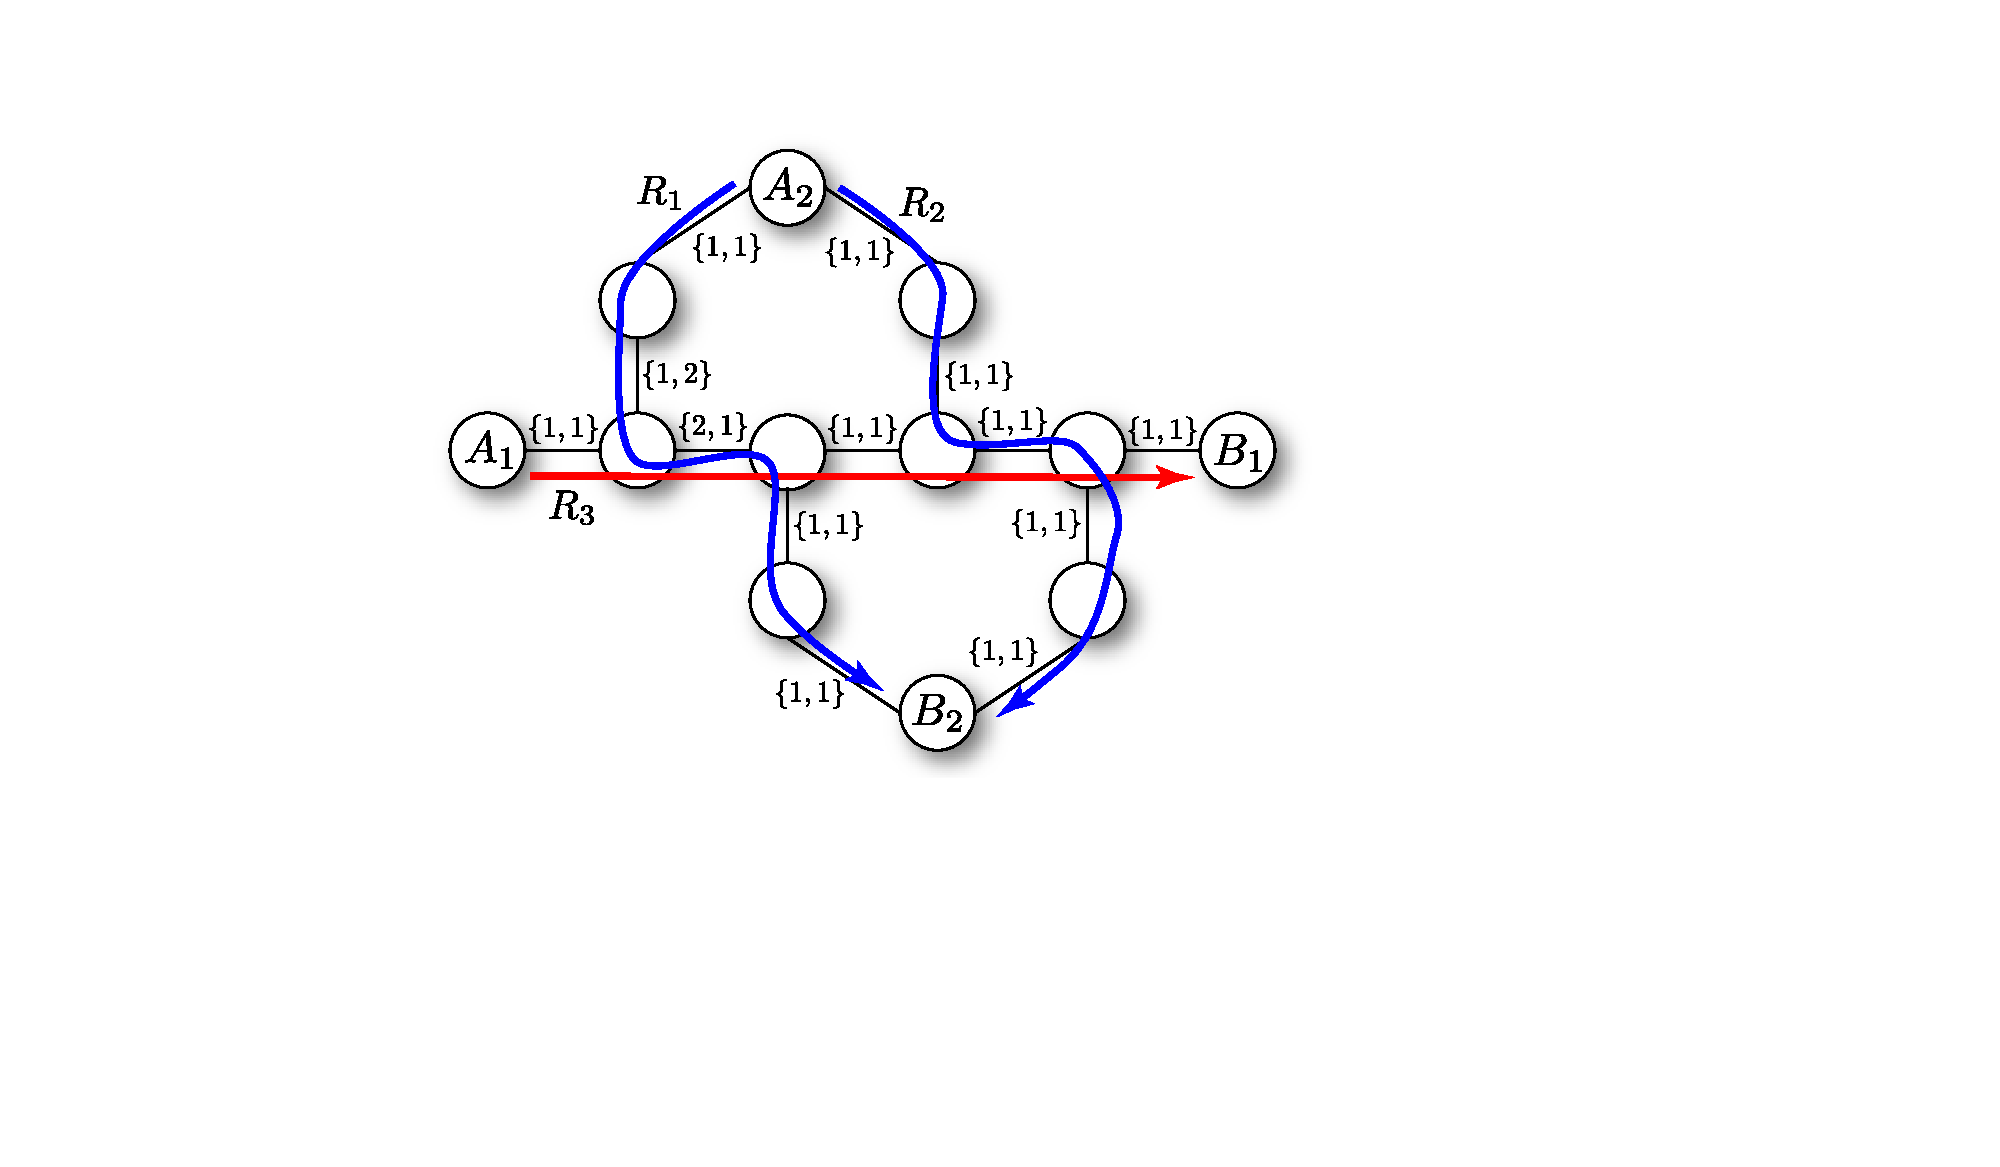
\includegraphics[width=\columnwidth]{conflict}
\caption{A simple network with two competing pairs of senders and receivers, \mbox{$A_1\to B_1$} and \mbox{$A_2\to B_2$}. Edges are labelled by \mbox{$\{b,d\}$}, where $b$ is the bandwidth of the link (i.e number of states that can be communicated simultaneously), and $d$ is the cost associated with the link, e.g loss in dB). (blue line) $R_1$ and $R_2$ are two routes from $A_2\to B_2$. Either of these routes could be declared optimal, depending on the choice of cost function. (red lines) $R_3$ is the optimal route from \mbox{$A_1\to B_1$}.} \label{fig:conflict}
\end{figure}

Generalising this to any number of users is a straightforward extension to the route optimisation problem, incurring a higher computational overhead due to the increased optimisation complexity.

In the upcoming sections we discuss multi-user strategies in more detail. None of these are true {\sc Global} strategies, but nonetheless address some of the problems facing {\sc Local} strategies mentioned above.

\subsection{Round Robin} \label{sec:round_robin}

Perhaps the simplest and most elegant multi-user scheduling strategy is to borrow from the idea of time-division multiplexing for preemptive multitasking employed by UNIX operating systems. Here we simply put all live packets in a list, and go through the list, one-by-one, giving each packet an equal time-share of network resources, independent of costs. The algorithm for this is shown in Alg.~\ref{tab:round_robin}.

\begin{table}[!htb]
\fbox{\parbox{0.965\columnwidth}{\tt
function Strategy.RoundRobin(Packets):
\begin{enumerate}
    \item foreach(packet in Packets) \{
        \setlength{\itemindent}{.2in}
                \item currentNode = packet.RoutingQueue.Pop()
        \item shortestRoute = \\
        ShortestPath(currentNode,packet.Recipient)
        \item packet.RoutingQueue.Flush()
        \item packet.RoutingQueue.Push(shortestRoute)
    \setlength{\itemindent}{0in} \}
    \item $\Box$
\end{enumerate}}}
\caption{In the {\sc Round Robin Strategy} we simply iterate through the list of active packets, with no regard for any metrics, or conflicts between them. Rather, we strive for perfect time-sharing equality, and every packet entirely ignores the actions of all other packets.} \label{tab:round_robin}
\end{table}
The {\sc Round Robin} strategy can be considered base skeleton code for more sophistic algorithms to build upon.

While such a protocol clearly ensures scheduling that gives all packets attention, it is the perfect example of an algorithm subject to the resource allocation imbalance discussed in Sec.~\ref{sec:two_user}. Specifically, the routes being followed by some packets may systemically receive more favourable treatment than others, based on the ordering of the list of packets. Also, equal timesharing fails to accommodate for the fact that some routes are inherently more costly than others and deserve a greater share of network resources.

\subsection{Data Priority} \label{sec:data_priority}

Are all men created equal? No. Some packets may inherently be more important than others, and ought to receive priority when allocating network resources. A simple variation on the {\sc Round Robin} strategy is to, before iterating through the list of packets, order them according to a {\sc Priority} attribute. Thus, when applying a shortest-path algorithm, it is deemed most important to minimise the costs of the more important packets.

This is trivially achieved by taking the existing {\sc Round Robin} strategy, and first ordering the packet list by their priority attributes, i.e by inserting a new line 1, \mbox{\tt Packets.SortByPriority()}.

\subsection{Randomisation} \label{sec:random}

The imbalance issue facing the {\sc Round Robin} strategy (Sec.~\ref{sec:round_robin}) may be most trivially addressed using randomisation of the strategy, such that routes are optimised in an order chosen randomly each time. This would allow the different sender/receiver pairs to have equal access to network resources, when averaged over many network uses.

This is also straightforward variation of the {\sc Round Robin} strategy, achieved by first randomising the list of packets before the other stages, i.e insert a new line 1, \mbox{\tt Packets.RandomizeOrder()}.

\subsection{Cost Priority} \label{sec:cost_priority}

The {\sc Random} strategy overcomes one key problem facing any {\sc Local} optimisation strategy. But it is nonetheless merely a mild variation on the {\sc Round Robin} strategy, guaranteeing equal time-share to each route. But does equal time-sharing actually represent the best allocation of resources?

It isn't just the order in which routes are chosen which creates imbalance between users. The costs and attributes of the routes themselves is inevitably biased more in favour of some users than others. To accommodate this we now introduce the {\sc Cost Priority} strategy. Here, rather than prioritising packets on a random basis, or according to a fixed, predetermined priority attribute, we do so according to their net accumulated cost. Those who have accumulated the highest cost will subsequently be treated with highest priority. This strategy effectively introduces a negative feedback loop into resource allocation, creating a self-regulating (and hopefully stable!) time-multiplexed packet-switched network. The pseudo-code for the {\sc Cost Priority} strategy is shown in Alg.~\ref{tab:cost_prior_alg}.

\begin{table}[!htb]
\fbox{\parbox{0.965\columnwidth}{\tt
function Strategy.CostPriority(Packets):
\begin{enumerate}
    \item packetsAndCosts = []
    \item foreach(packet in Packets) \{
        \setlength{\itemindent}{.2in}
        \item cost = costFunction(packet)
        \item packetsAndCosts.Append([packet,cost])
    \setlength{\itemindent}{0in}
    \item     \}
    \item sorted = \\
        SortByCostDescending(packetsAndCosts)
    \item foreach(packet in sorted) \{
        \setlength{\itemindent}{.2in}
        \item currentNode = packet.RoutingQueue.Pop()
        \item shortestRoute = \\
        ShortestPath(currentNode,packet.Recipient)
        \item packet.RoutingQueue.Flush()
        \item packet.RoutingQueue.Push(shortestRoute)
    \setlength{\itemindent}{0in}
    \item \}
    \item $\Box$
\end{enumerate}}}
\caption{The {\sc Cost Priority Strategy} scheduling algorithm that gives highest routing priority to {\sc Packets} with the highest accumulated cost (i.e which have suffered the most). The as-yet undefined {\tt costFunction()}, which refers to $f_\mathrm{cost}$ from Eq.~\ref{eq:net_cost_R}, is where the details of the priority decisions are made, which could be entirely arbitrary. In this example, the shortest route is recalculated at each step, based on the expectation that network metrics are dynamic.} \label{tab:cost_prior_alg}
\end{table}

This is an example of a \emph{greedy} optimisation algorithm, which attempts to optimise routing by always optimising the most desperate packets first, in descending order down to the least. It is well-known that greedy algorithms often do not find global optima. Nonetheless, this approach improves on the previous multi-user protocols.

Let us consider a simple example scenario. Imagine we begin with an ordinary network graph, with edges weighted by costs and attributes. For generality, we will additionally assume the available network resources are very dynamic and unpredictable. The costs associated with links are at the whim of market forces we do not understand. And, for the sake of example, and to make matters worse, the links have been very unreliable lately, and are routinely dropping in and out -- `blackouts'. This effectively rules out \emph{a priori} route optimisation, requiring something dynamic.

There are many users on the network, with many active packets at any give time, but because of the constant oscillations in network resources, some {\sc Packets} have received second-class treatment, and through neglect accumulated an unfair share of state degradation. This simple toy model is, at least qualitatively, something that could arise quite naturally in networks with constrained or unreliable resources.

Let us define an example {\sc Cost Priority} strategy using the following:
\begin{itemize}
\item {\sc Latency Cost}: How long has the packet has been in transit for? This is actually a very general cost metric, since any other cost metric measured in units per time will be directly proportional to this metric. That is, fidelity, purity, efficiency, and so on, all mirror this metric when expressed on a decibel scale. Of course, the same strategy could have easily been applied to any other cost metric.
\item {\sc Blackout Attribute}: Is our unreliable link actually working right now? A given link will have probability $p_\mathrm{op}$ of being operational at any given time, chosen independently for each link at each clock-cycle. The {\tt Attributes.Update()} function from Alg.~\ref{tab:transport_alg} is responsible for implementing this.
\item \mbox{\sc Cost Function} ($f_\mathrm{cost}$, {\tt costFunction()} in Alg.~\ref{tab:cost_prior_alg}): The strategy must make sensible decisions based upon only the above two parameters. Because the previously mentioned generality of the {\sc Latency} metric, we would like the net cost to directly reflect this metric, but only of course, if the link is operational. If it is not, then that link must be ruled out entirely by assigning it an infinite cost. Thus, we simply choose,
\begin{align}
\mathcal{S} : f_\mathrm{cost}(c,a) = \left\{
\begin{array}{l l}
c & \quad \mathrm{if}~ a=\mathrm{\tt True} \\
\infty & \quad \mathrm{if}~ a=\mathrm{\tt False} \\
\end{array} \right..
\end{align}
Note that different packets could be associated with different net cost functions, $f_\mathrm{net}$, to accommodate for the different QoS requirements of different users and messages.
\end{itemize}

In other words, the net cost is taken directly from the underlying cost metric, and modulated by an attribute, yielding a net cost for each packet, which is used to determine which packets receive priority.

This provides us with a simple illustration of how costs and attributes can compliment one another to yield meaningful strategies, that improve network performance over na\"ive, but well-intentioned, time-sharing approaches.

\subsection{All or Nothing} \label{sec:all_or_nothing}

In some cases, end user applications may have strict QoS constraints associated with any data they receive. For example, in a time-critical enterprise, say high-frequency trading, receiving information a millisecond too late is worthless, and it would be best to discard the out of date information to free up bandwidth for the next round of information. In such a context, the {\sc Strategy} will apply hard boundaries on QoS metrics, discarding anything violating it. The algorithm is summarised in Alg.~\ref{tab:all_or_nothing}.

\begin{table}[!htb]
\fbox{\parbox{0.965\columnwidth}{\tt
function Strategy.AllOrNothing(Packets, threshold):
\begin{enumerate}
    \item foreach(packet in Packets) \{
        \setlength{\itemindent}{.2in}
        \item cost = costFunction(packet)
        \item if(cost $\geq$ threshold) \{
        \setlength{\itemindent}{.4in}
            \item packet.Sender.Notify({\sc Failure})
            \item packet.Recipient.Notify({\sc Failure})
            \item Packets.Discard(packet)
                    \setlength{\itemindent}{.2in}
            \item \}
        \setlength{\itemindent}{0in}
    \item \}
    \item $\Box$
\end{enumerate}}}
\caption{The {\sc All or Nothing Strategy}. If the net cost of a packet exceeds a certain {\tt threshold}, it is discarded outright, and the sender and recipient notified.} \label{tab:all_or_nothing}
\end{table}

\subsection{Optimal Flow}

In Sec.~\ref{sec:flow_networks} we introduced flow networks as a means for analysing networks where maximising network flow (throughput) is the primary objective. Formulating our quantum networks in this manner is extremely convenient since, combined with our existing definitions for cost metrics and attributes, we can easily exploit a plethora of known results from flow network theory.

As an example of how load allocation might be applied in a simple network, consider again the network shown in Fig.~\ref{fig:simp_route_opt}, where the edge weights are regular cost metrics (not capacities). Alice wishes to send two packets to Bob, simultaneously if possible. Clearly she would transmit her first packet over the \mbox{$A\to F\to B$} route, since this has lowest cost. But let us assume that every link has a maximum capacity of one packet per unit time. In this case Alice will be unable to send her second packet via the same route and must instead resort to using \mbox{$A\to C \to B$} or \mbox{$A\to D\to B$}. The optimisation is straightforward in this instance. However, in general these types of optimisations are somewhat more involved.

These scenarios are handled by flow network optimisation algorithms, of which there are many. We discuss a few of the most relevant ones for our purposes in Sec.~\ref{sec:graph_theory}. Note that these algorithms are {\sc Global} optimisation algorithms, requiring complete knowledge of the status of the entire network to perform the optimisation.

The routing strategy is very straightforward, shown in Alg.~\ref{tab:opt_flow}, since the {\sc Global} flow-optimisation algorithm completely specifies the entire configuration of routes through the network.

\begin{table}[!htb]
\fbox{\parbox{0.965\columnwidth}{\tt
function Strategy.OptimalFlow(Packets):
\begin{enumerate}
    \item routes = Packets.OptimalFlowRoutes()
    \item foreach(packet in Packets) \{
        \setlength{\itemindent}{.2in}
                \item packet.RoutingQueue.Flush()
                \item packet.RoutingQueue.Push(routes[packet])
    \setlength{\itemindent}{0in} \}
    \item $\Box$
\end{enumerate}}}
\caption{A generic optimal flow routing strategy. {\sc Packets} is the array of all packets that ought to be transmitted simultaneously, which are collectively optimised using some flow optimisation algorithm before undergoing transport.} \label{tab:opt_flow}
\end{table}

\section{Extensibility of QTCP} \label{sec:c_vs_a}

In Sec.~\ref{sec:costs} we introduced the notion of the \emph{costs} and \emph{attributes} of links in a classical network, and in Sec.~\ref{sec:quantum_meas_cost} generalised these notions to the quantum case. In Sec.~\ref{sec:packet_header} we described the header format for quantum packets.

The {\sc Costs} and {\sc Attributes} fields within the {\sc Header} are very powerful data structures, implemented as ordered sets of arbitrary dimension, comprising arbitrary data fields. The intention here is to allow QTCP to be extensible into the future, with the addition of new data structures into the protocol. These can be custom designed to, in conjunction with appropriate routing strategies and cost functions, influence the operation of QTCP completely arbitrarily, and easily implement entirely different quantum networking paradigms than presented here.

{\sc Costs} naturally capture characteristics of the network that accumulate additively along routes, whereas {\sc Attributes} capture any other characteristics that aren't additive. A network needn't have both costs \emph{and} attributes. It may have one or the other, or both, but not neither, since there must be some measure by which to judge routes.

\section{Interconnecting Networks}

Any global-scale network will inevitably comprise participants choosing to go about things their own way. The physical architecture and medium may vary from one subnetwork to the next, as may the QTCP policies they adopt. The key then is to construct efficient \emph{interconnects} between different levels of the network hierarchy, each of which may subscribe to their own QTCP policies and cross between different physical mediums. Note that the QTCP protocol presented here does not enforce any particular networking policies, but rather provides a high-level framework that can be customised essentially arbitrarily.

For example, the cost metrics and attributes employed at the intercontinental level would most certainly be very different to those in a small LAN. A small LAN might be running applications whereby they can easily reproduce packets and thereby tolerate packet loss. But for a warehouse-scale commercial quantum computing enterprise, responsible for performing one stage of a distributed quantum computation, the loss of a single packet could be extremely costly, requiring the entire computation to be performed completely from scratch due to no-cloning and no-measurement limitations, something that may not come cheaply.

Such interconnects will typically comprise a combination of:
\begin{itemize}
\item Packet switching: such that packets can be arbitrarily switched between the different levels of the network hierarchy.
\item Physical interface: interconnect may be switching between different media. Such physical interfaces have costs associated with them. For example, coupling between free-space and fibre is typically very lossy.
\item Quantum memory: such that data can be buffered while it awaits its turn at being switched between networks, as different networks may have different loads and operate at different clock rates.
\item Packet format conversion: different levels of the network hierarchy may be employing entirely different cost metrics, attributes, and cost functions, requiring packet headers to be reformatted upon switching between networks.
\end{itemize}

The packet switching and quantum memory are implemented as quantum processes at nodes, using the usual quantum process formalism. The physical interface between different mediums, if there is one, could be very diverse, encompassing many types of physical systems, but can always be characterised using the quantum process formalism. Packet headers, which contain all formatting, cost, and routing information are represented entirely classically and communicated entirely by the classical network. Thus, this operation also takes place at nodes, but no quantum processes are taking place.

\section{Network Topologies}

As quantum (or classical) networks inherently reside on graphs, it is important to introduce some of the key graph structures of relevance to networking and some of their properties of relevance to quantum networking protocols.

In principle a network could be characterised by any connected graph whatsoever. However, there are certain structures and patterns that emerge very frequently and deserve special attention.

It is paramount that QTCP protocols have the capacity to deal with the diverse network topologies that are likely to present themselves in the future real-world quantum internet. Thankfully, the most important graph-theoretic algorithms that we rely on in our QTCP protocol (see Sec.~\ref{sec:graph_theory}) are computationally efficient for \emph{arbitrary} graph topologies, even more so for certain classes of graphs exhibiting particular structure, such as tree graphs or complete graphs.

We will now review some of the graph structures most likely to arise in quantum networks.

\subsection{Complete}

The complete graph, denoted $K_{|V|}$, is a $|V|$-vertex graph where every vertex has an undirected link to every other. From a networking point of view, this can be regarded as the extremity of Point-to-Point (P2P) networking, whereby every node has a direct link with every other. This type of topology could arise in large broadcast-type networks, like Ethernet, where everyone can speak directly with everyone else directly by shouting loud and often enough, so as to overcome collisions (see Sec.~\ref{sec:collision} for further details on collision handling). Fig.~\ref{fig:complete_graph} illustrates the $K_{15}$ graph. The number of edges scales as $O(n^2)$. Clearly route-finding is trivial, since there is always a direct link from sender to receiver, with no possibility of collisions with other packets, requiring $O(1)$ search time (assuming all users are communicating only via their direct links with one another, which may not strictly be the case when costs are factored into strategies).

Assuming packets always traverse the direct links to their destinations, the net cost of routes does not accumulate, but is limited to the cost of the single traversed link. This is the minimum possible cost, but comes at the expense of requiring the most elaborate and expensive network.

In reality, this type of topology might arise quite naturally on small Local Area Networks (LANs), but will most certainly never, on its own, form the basis of a large-scale, international quantum internet, as the number of long-distance links that would have to be implemented would be prohibitively costly.

\begin{figure}[!htb]
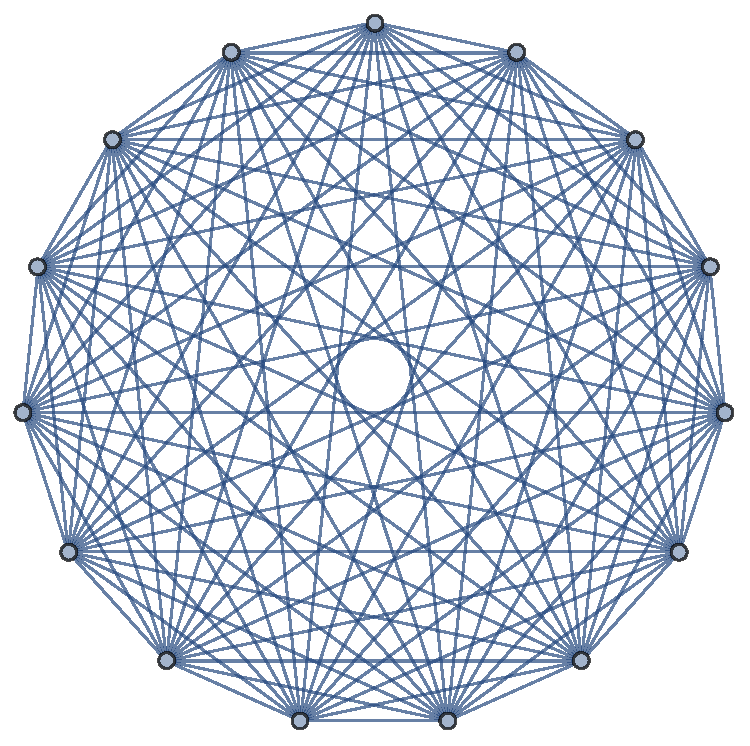
\includegraphics[width=0.7\columnwidth]{K_15}
\caption{The 15-vertex complete graph, $K_{15}$. Every vertex has an edge to every other, with a total of 105 edges.} \label{fig:complete_graph}
\end{figure}

\subsection{Lattice}

A lattice graph is simply an \mbox{$n\times m$} lattice of vertices (of any geometry, e.g squares), connecting each vertex to its immediate geometric neighbours. This type of graph is useful when link costs are measured in terms of Euclidean distances, and nodes have nearest neighbour links. An example is shown in Fig.~\ref{fig:lattice}.

\begin{figure}[!htb]
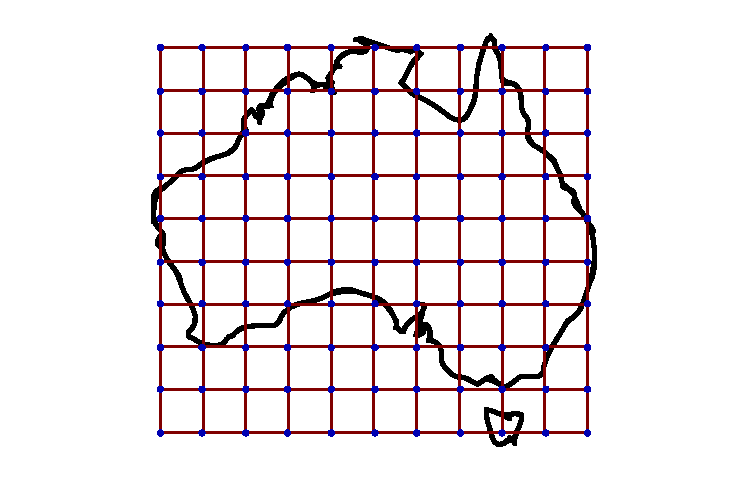
\includegraphics[width=0.7\columnwidth]{lattice}
\caption{A \mbox{$10\times 11$} square lattice graph, and how it might represent a network topology with geographically associated costs. Notice that Hobart has no internet connection (why even include Tasmania at all?).} \label{fig:lattice}
\end{figure}

A slightly distorted lattice graph, in which vertices have been dragged around geometrically to match, for example, cities within a country, closely resembles the topology of the network. Similarly, if the nodes represent houses in the street layout of a highly regular city like Manhattan, a lattice may be a good approximation.

In the case of a balanced lattice, in which all edges are of equal weight, the cost of a route is the sum of the number of steps in the vertical, and number of steps in the horizontal directions, also known as the Manhattan, or $L_1$ distance,
\begin{align}
L_1 = |x_\mathrm{start} - x_\mathrm{finish}| + |y_\mathrm{start} - y_\mathrm{finish}|.
\end{align}
In this case, route finding is simplified, since \emph{all} routes, which strictly traverse in one direction vertically and one direction horizontally, are optimal and of equal distance.

\subsection{Tree} \label{sec:tree_graph}

A tree is a graph containing no cycles, only \emph{branches}. There are many uses for tree graphs, but one property is of particular convenience in many applications: because the graph is acyclic, there is always exactly one path from any vertex to any other. This mitigates the need for shortest-path algorithms designed for general graphs, and simplifies route-finding algorithms (to be discussed in Sec.~\ref{sec:path_exp}).

Trees are specified entirely by \emph{branching parameters} ($b_i$) -- the number of child nodes emanating from a given node, $i$. In general, branching parameters may be distinct for each node, although often trees with symmetries in their branching structures are considered, such as the balanced trees discussed in Sec.~\ref{sec:bal_tree}. A node terminates a branch if its branching parameter is zero (i.e it has no children). The \emph{depth} ($d$) of a tree is the maximum number of steps from the root node to a terminating node with no children. The depth scales between \mbox{$d=|V|$}, for the trivial linear tree (\mbox{$b_i=1$}), and \mbox{$d=O(\mathrm{log}|V|)$} for non-trivial branching parameters (i.e \mbox{$b_i\neq 1$}). The worst-case number of edges that must be traversed to reach any vertex from any other is twice the depth, which implies that cost metrics scale as at most \mbox{$c=O(\mathrm{log}|V|)$}. Trees are the most frugal graphs in their number of edges, which are fixed at \mbox{$|E|=|V|-1$}, irrespective of the branching parameters, since because the graph is strictly acyclic, every addition of an edge requires the addition of a single vertex.

\subsubsection{Balanced Tree} \label{sec:bal_tree}

A balanced tree is a tree with a regular, self-similar structure, in which every node (up to a given depth) is the parent of the same number of sub-nodes, all separated by the same, but equal or smaller edge weights. That is, the network has a hierarchical structure, dividing into sub-networks of decreasing size. Such a network is characterised by just two parameters -- the branching parameter, $b$, and the depth, $d$. Some examples of balanced trees with different $b$ and $d$ are shown in Fig.~\ref{fig:tree_example}.

\begin{figure}[!htb]
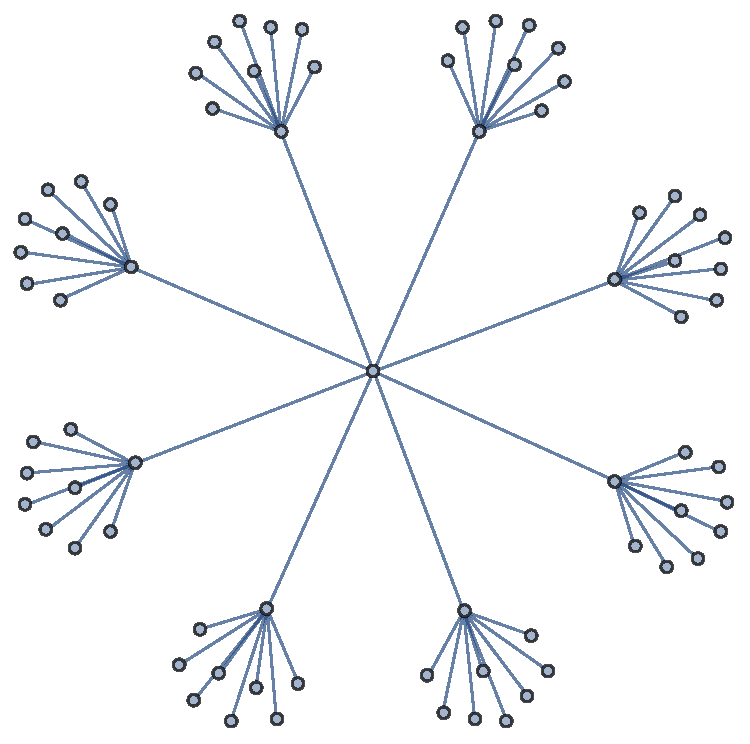
\includegraphics[width=0.75\columnwidth]{tree_3_8} \\
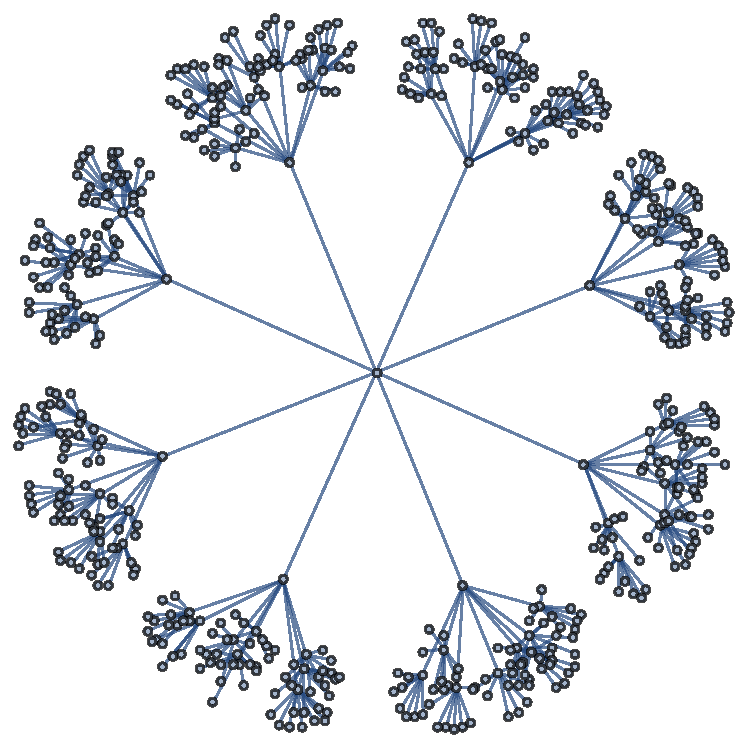
\includegraphics[width=0.75\columnwidth]{tree_4_8} \\
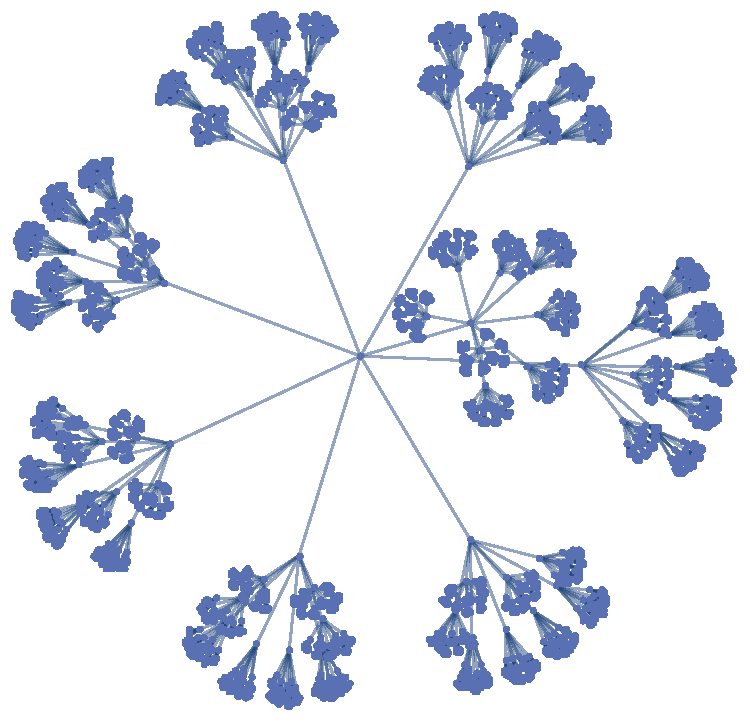
\includegraphics[width=0.75\columnwidth]{tree_5_8}
\caption{Balanced tree graphs with branching factor $b=8$, and depths $d=3,4,5$ (top to bottom). Despite having no redundant paths, the hierarchical structure of balanced trees somewhat resembles that of real-world networks, which are typically decomposed into a pyramid scheme of progressively smaller sub-networks.} \label{fig:tree_example}
\end{figure}

This type of structure is natural in many realistic scenarios. Consider for example a network containing a hierarchy of clusters of nodes representing a Local Area Network (LAN), followed by a neighbouring internet router, followed by a city-wide router, followed by a country-wide router. In such a case, this type of general structure is typical.

\subsubsection{Random Tree}

While balanced trees accurately capture the hierarchical nature of realistic networks, they are somewhat contrived in their perfect symmetry. The sub-networks in a given network are not likely to actually all be identical. Random trees are perhaps more realistic, in that their tree structure captures the hierarchical nature of real-world networks, and also their highly ad hoc nature.

To construct a random tree we simply randomly choose a branching parameter, up to some maximum, for every node. When a node has \mbox{$b_i=0$}, it terminates the lineage. Some examples of random trees are shown in Fig.~\ref{fig:random_tree}.

\begin{figure}[!htb]
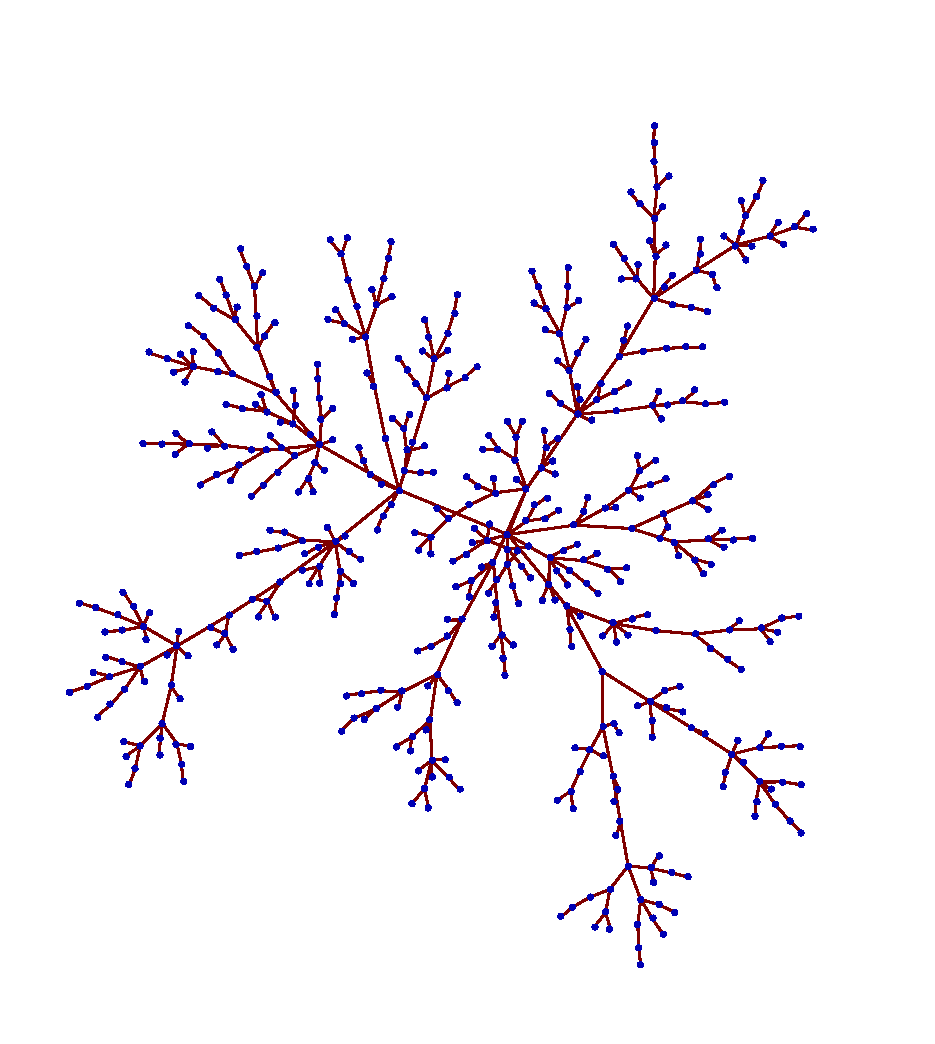
\includegraphics[width=\columnwidth]{random_tree_1} \\
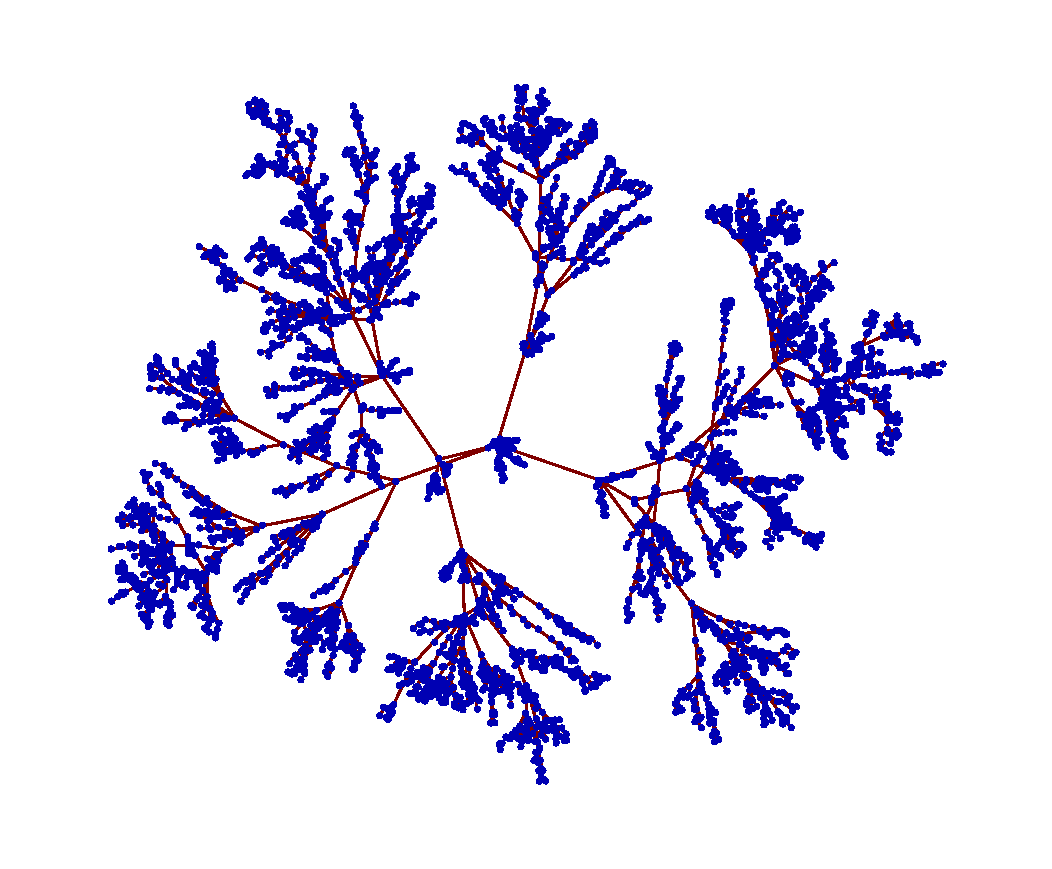
\includegraphics[width=\columnwidth]{random_tree_2}
\caption{Random trees with different randomised branching parameters (higher $b$ at bottom). When a node has zero branches, it terminates the branch. This type of graph topology qualitatively captures the hierarchical, yet ad hoc qualities of many real-world networks, and may act as a useful test model for simulations.} \label{fig:random_tree}
\end{figure}

\subsubsection{Minimum Spanning Tree} \label{sec:graph_MST}

A \emph{spanning tree} $S$, of a graph $G$, is a tree subgraph \mbox{$S\subset G$}, containing every vertex of $G$. The \emph{weight} of a spanning tree is the sum of all its constituent edge weights. Thus, the \emph{Minimum Spanning Tree} (MST) is a spanning tree that minimises weight. An example is shown in Fig.~\ref{fig:mst}. See Sec.~\ref{sec:min_tree} for a discussion on MST algorithms.

\begin{figure}[!htb]
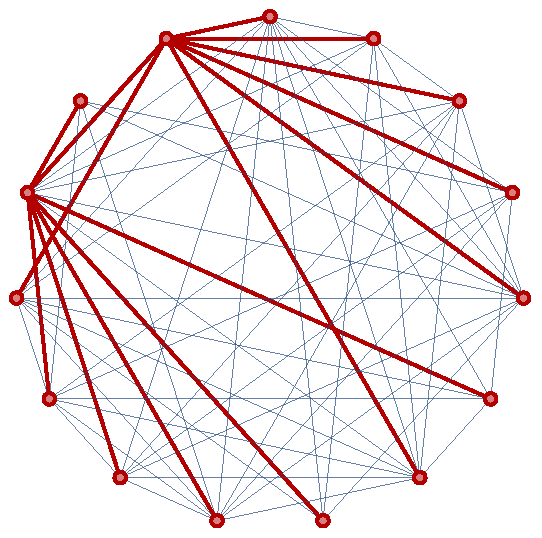
\includegraphics[width=0.8\columnwidth]{mst}
\caption{A random graph (blue) with its MST highlighted (red).} \label{fig:mst}
\end{figure}

The calculation of MSTs is most likely to come into consideration when actually performing the initial construction of networks, where we wish to connect all nodes in the network, but using the most frugal possible physical resources. MSTs serve this purpose, and since they are trees, inherit all the same properties of tree networks.

\subsubsection{The Internet Webgraph}

Of course, all the topological structures described until now are in-principle constructs. Of most relevance is the \emph{Webgraph}, the graph of the actual internet. Fig.~\ref{fig:webgraph} illustrates the Webgraph via the Internet Mapping Project. The combination of random, densely and sparsely connected, and tree structures, and clear hierarchical structure are all evident. This encourages our intuition of the different types of structures present in realistic networks.

\begin{figure}[!htb]
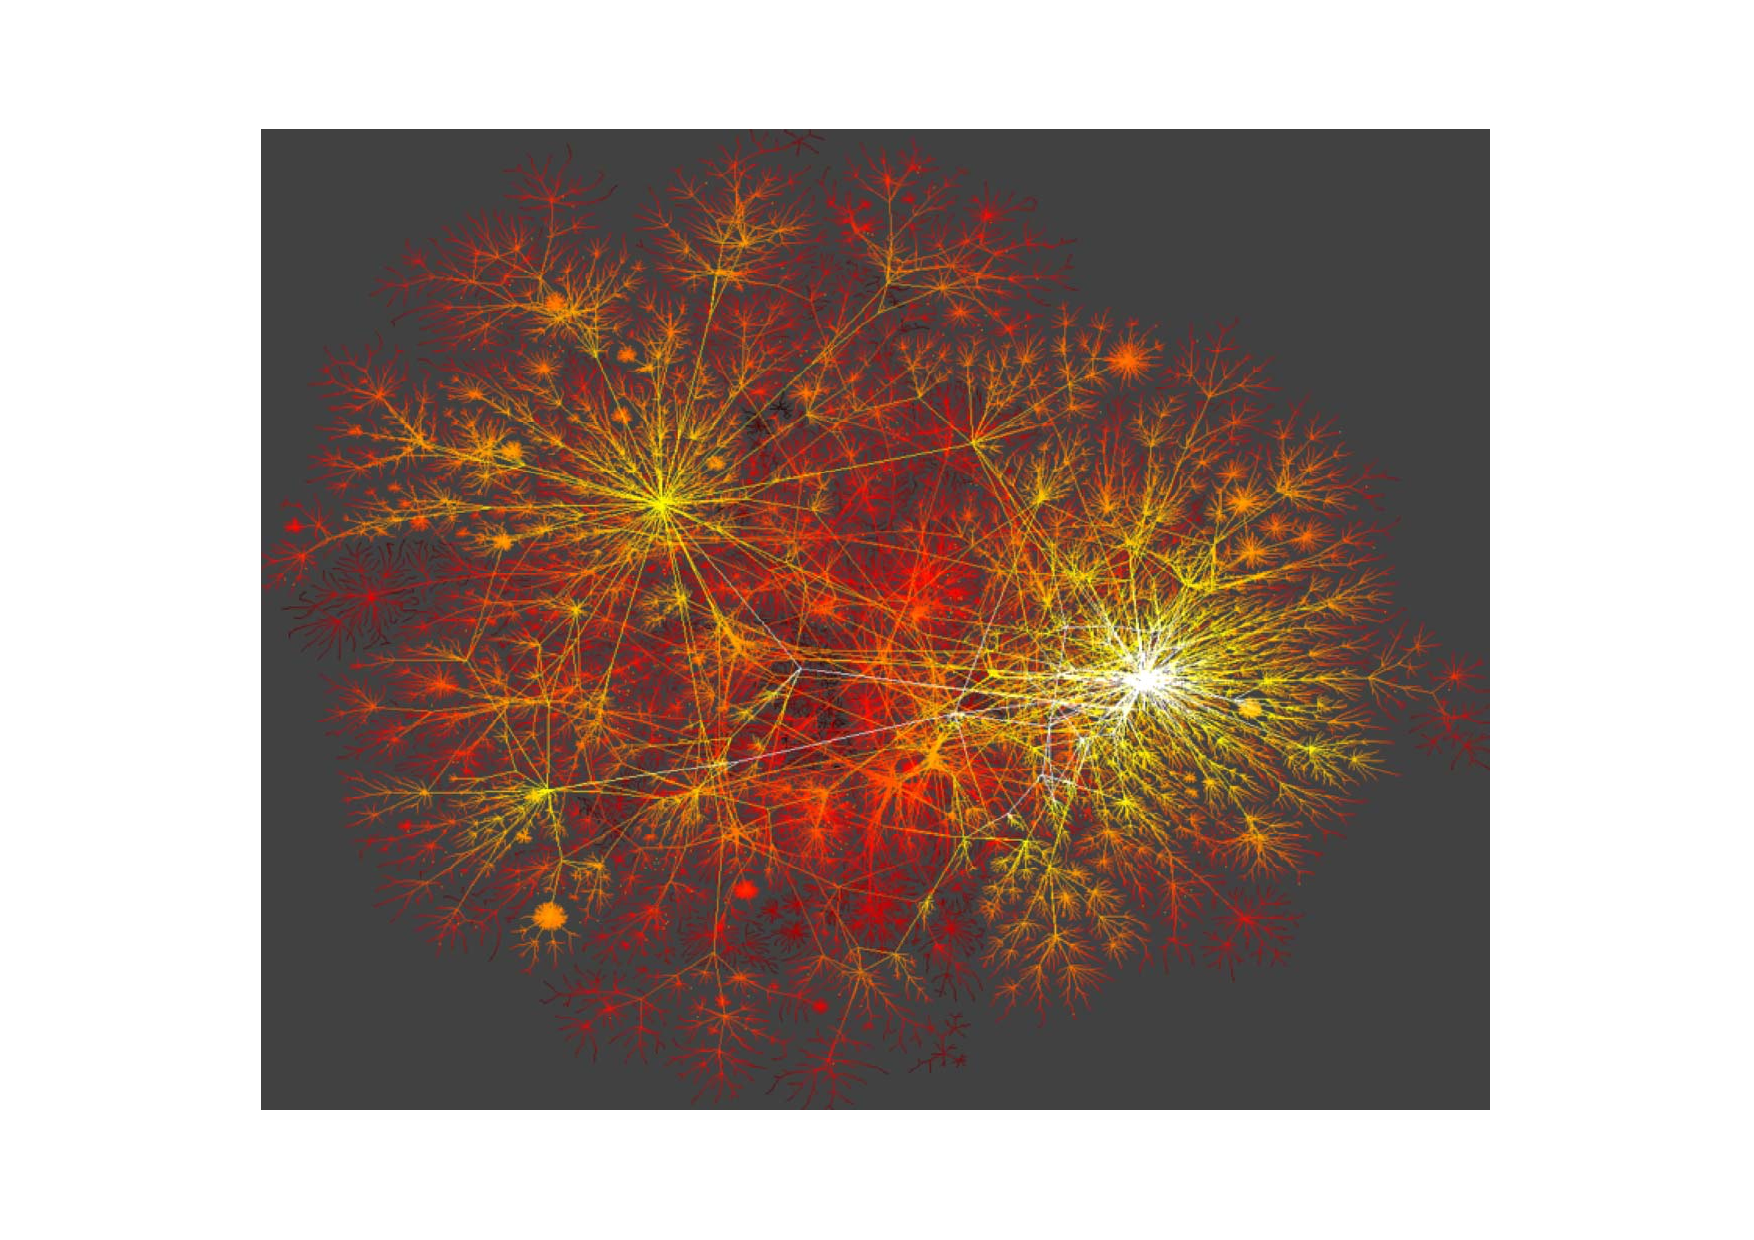
\includegraphics[width=\columnwidth]{webgraph}
\caption{The real-world webgraph, capturing the high-level structure of the global internet. A random tree structure is visually apparent. \comment{CITE THE SOURCE! Is it open source?}} \label{fig:webgraph}
\end{figure}

\subsection{Random}

A variation on the complete graph, $K_{|V|}$, is to instead have a randomised implementation of it, whereby each of the possible edges in $K_{|V|}$ occurs with probability \mbox{$0\leq p_\mathrm{edge}\leq 1$}. We would thereby be able to tune between the complete graph and the completely disconnected graph, representing a randomly connected network with arbitrary average connectivity. Specifically, the average number of links emanating from any node is \mbox{$e_\mathrm{av} = (|V|-1)p_\mathrm{edge}$}. Note that random graphs might be disjoint, making them inappropriate for many networking applications. For asymptotically large random graphs, \emph{percolation theory} provides thresholds for $p_\mathrm{edge}$ such that they remain connected \cite{???}. Fig.~\ref{fig:random_graph} illustrates several graphs with different edge connectivity probabilities.

\begin{figure}[!htb]
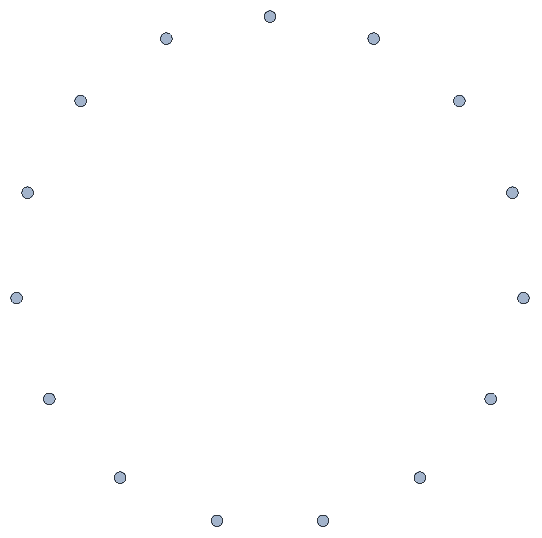
\includegraphics[width=0.6\columnwidth]{random_0}
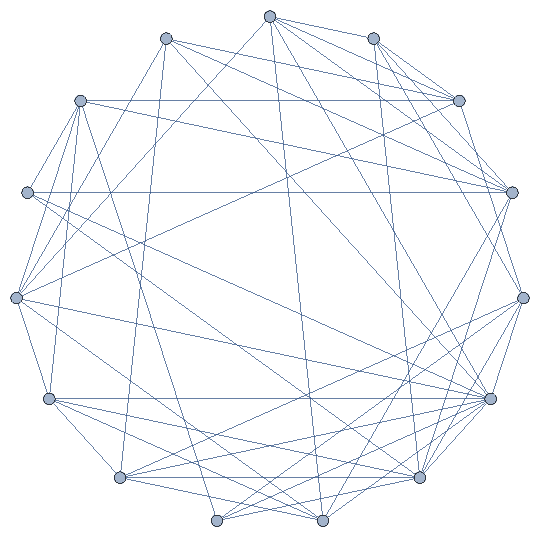
\includegraphics[width=0.6\columnwidth]{random_05}
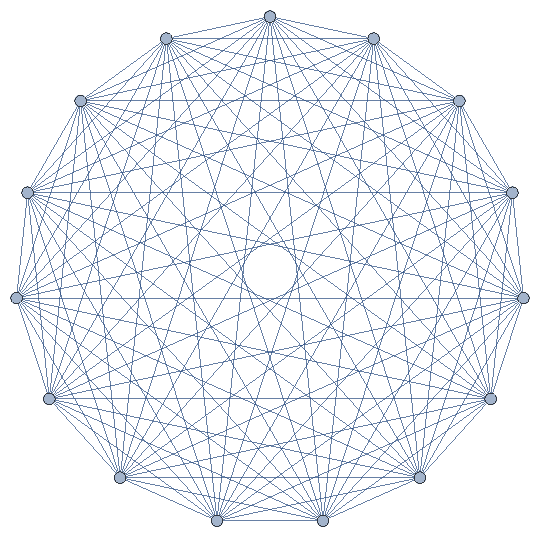
\includegraphics[width=0.6\columnwidth]{random_1}
\caption{The 15-vertex randomly-connected graph. This is the same as $K_{15}$ in Fig.~\ref{fig:complete_graph}, but where edges are present with probabilities \mbox{$p_\mathrm{edge}=0,0.5,1$} (top to bottom).} \label{fig:random_graph}
\end{figure}

Random graphs capture the ad hoc nature of networks that exhibit no planned structure, but are rather cobbled together in a completely improvised manner.

\subsection{Hybrid}

Real networks are highly unlikely to fit the exact form factor of any of the classes of graphs presented above. Rather, a truly global internet is inevitably going to comprise many sub-networks, each structured completely independently of one another, with little consistency or large-scale planning between them. Who thinks about the broader structure of the global internet when setting up their office network?

For example, at the global scale, it is entirely plausible that the internet might take on a random tree-like structure. But when we get down to a lower level, the tree structure vanishes and is replaced by all manner of different network topologies, run and maintained by different organisations in their own distinct ways.

Furthermore, the real-world internet is not simply a hierarchy of different types of well-known graph structures. Rather, it takes the form of `glued' graphs, whereby networks running over different media, or via different operators, each exhibit their own independent graph topologies, meeting at interconnect points that join the different networks. Typically this yields redundancy in the routes between different nodes.

This hybrid network topology is the norm today in our classical internet, and it is entirely foreseeable that a similar trend will emerge in the future quantum internet as quantum technologies become more mainstream, their networking less well structured, and competing, redundant links are in place.

\section{Network Algorithms} \label{sec:graph_theory}

Having introduced some of the more relevant graph structures, we now introduce some of the key graph theory algorithms that are of direct relevance to networking theory. In graph theory, many fundamental problems are believed to be computationally hard to solve. However, there are several important graph algorithms that are classically efficient to solve, and which are of great utility to us as network architects.

\subsection{Network Exploration \& Pathfinding} \label{sec:path_exp}

Here the goal is to systematically explore every vertex in an unknown graph exactly once, so as to reconstruct the entire network graph, or, to find a target node with unknown location (which can obviously be achieved if the former can be). The two main approaches are \emph{breadth-first-search} (BFS) and \emph{depth-first-search} (DFS) algorithms. In both cases we begin at a starting (root) node, from which we wish to explore the entire graph by only following edges.

In BFS we proceed from the root node to visit every one of its neighbours. Having done so, and created a list of those neighbours, we proceed onto the neighbours of the neighbours, and so on, until every vertex in the graph has been visited, or the target node found.

In DFS, on the other hand, we begin by following a single arbitrary path until we reach a dead-end, at which point we backtrack until we reach a branch leading to a vertex we hadn't previously visited.

Both BFS and DFS guarantee visiting every vertex in a connected graph, and do so using only nearest neighbour transitions. Such algorithms are therefore very useful for network discovery. The BFS algorithm is particularly applicable to pathfinding in ad hoc networks. Consider the situation where there is no central authority with full knowledge of the network, overseeing network operation. Rather, everyone needs to figure things out for themselves by speaking to their neighbours. This directly leads to a BFS search algorithm, where a node speaks to each of its neighbours in turn, who subsequently do the same thing. This can be naturally parallelised, as each node can be interrogating its neighbours independently.

Both BFS and DFS exhibit runtime \mbox{$O(|V|+|E|)$}, where $|V|$ and $|E|$ are the number of vertices and edges respectively. Thus, these graph exploration algorithms reside in the complexity class \textbf{P}, and are classically efficient.

\begin{figure}[!htb]
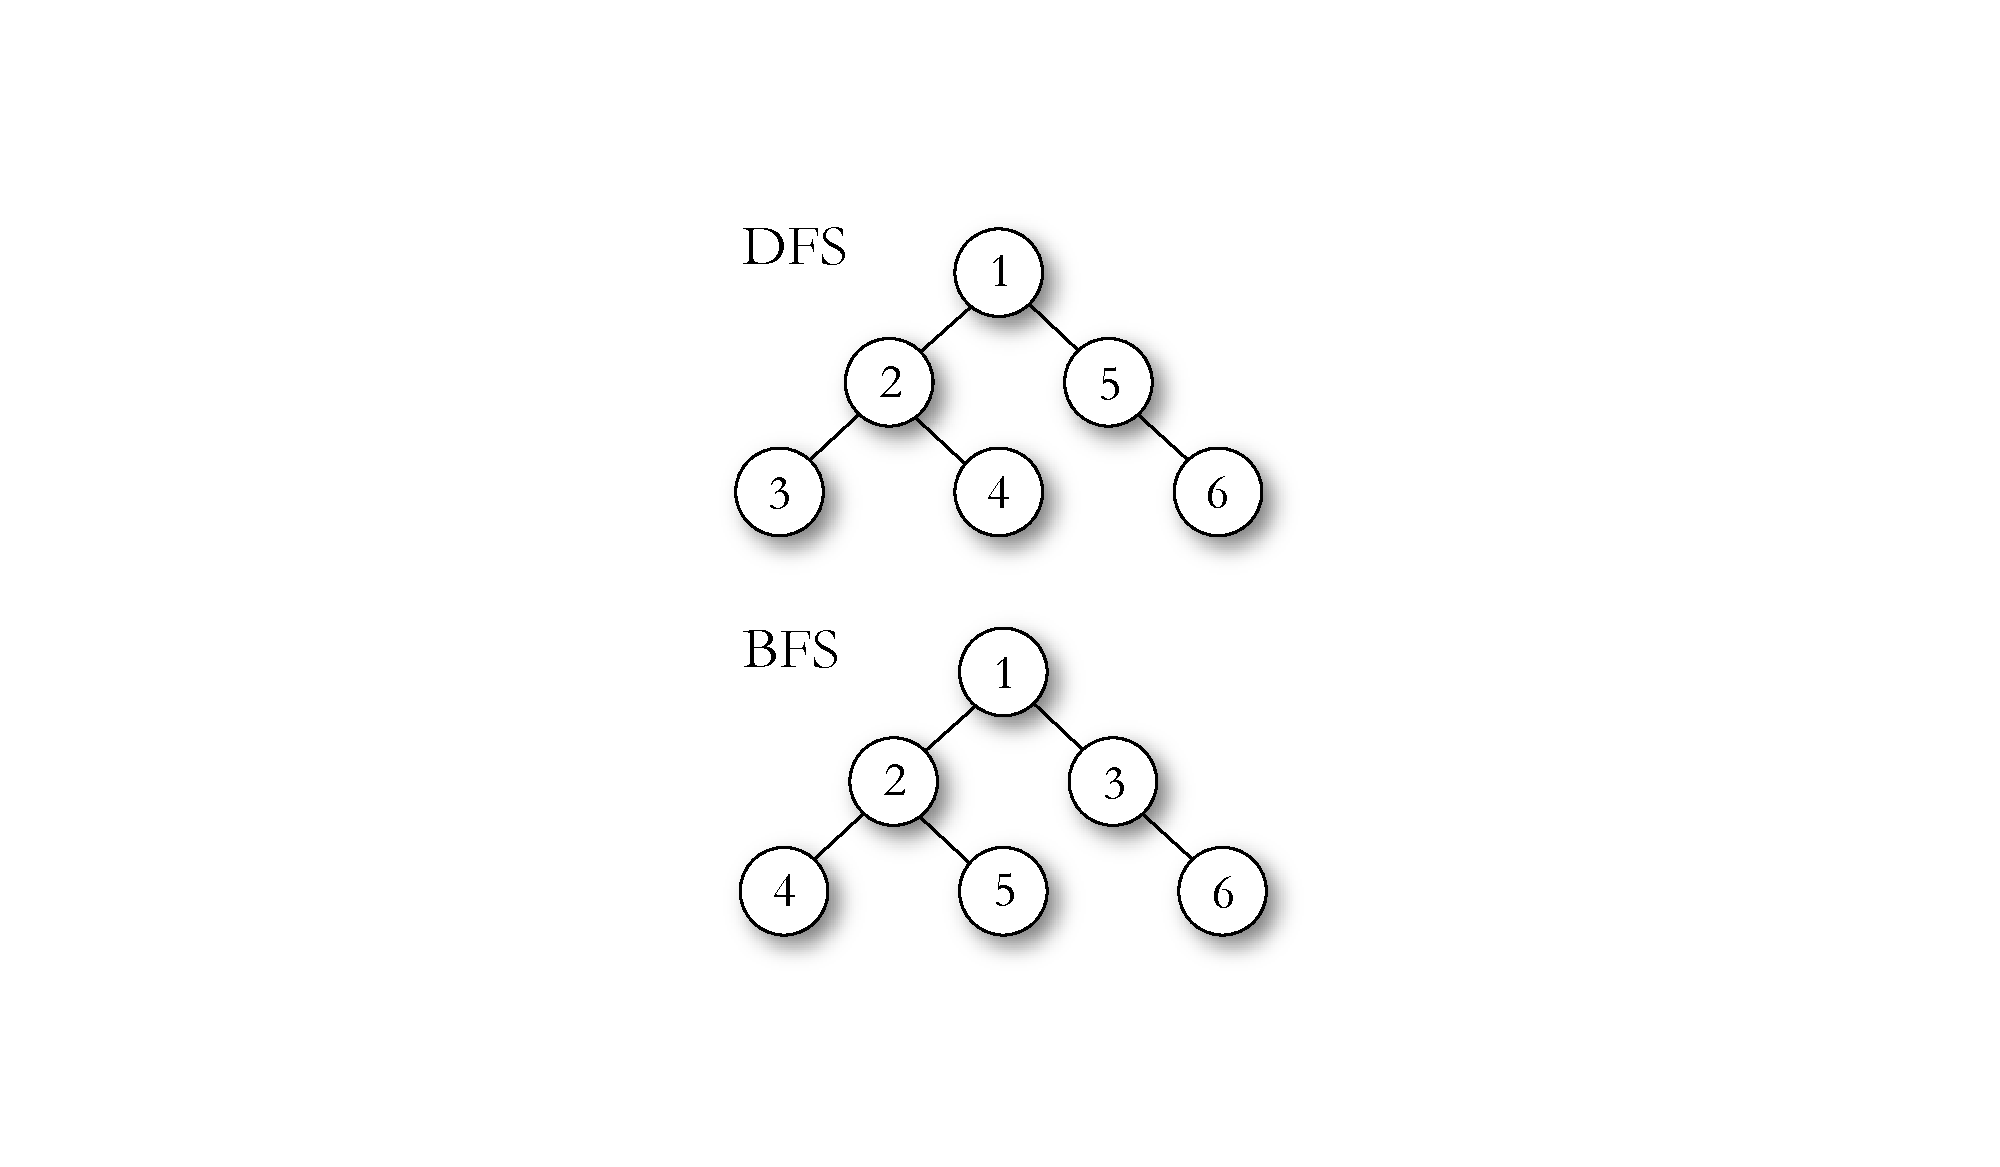
\includegraphics[width=0.6\columnwidth]{BFS_DFS}
\caption{Comparison of the order in which vertices are explored, using the depth-first search (DFS) and breadth-first search (BFS) algorithms, where vertex 1 is the root vertex.} \label{fig:BFS_DFS}
\end{figure}

\subsection{Shortest-Path} \label{sec:shortest_path}

In graph theory, the shortest-path problem is that of finding a subgraph of a given graph $G$, connecting two vertices, \mbox{$A\to B \subset G$}, such that the sum of its edge weights is minimised. In the context of our application to route-finding, this amounts to finding a route that minimises cost.

The first proven shortest-path algorithm was by Dijkstra \cite{bib:Dijkstra59}, which requires runtime $O(|V|^2)$, also residing in \textbf{P}. Subsequently, a number of improvements and variations on Dijkstra's algorithm have been proposed, most notably the $A^*$ algorithm, which has found widespread modern use.

Formally, let $\vec{R}$ be the set of all routes \mbox{$A\to B$}. Then,
\begin{align}
c_\mathrm{opt} = \min_{r\in R} \left(\sum_{i\in r} c_\mathrm{net}(i) \right),
\end{align}
where \mbox{$i\in r$} denotes the $i$th edge in the route $r$.

Fig.~\ref{fig:simp_route_opt} illustrates a directed, edge-weighted graph. A shortest-path algorithm applied between vertices $A$ and $B$ would return \mbox{$R_\mathrm{shortest} = A\to F\to B$} as the minimum cost route.

When introducing network graphs earlier, we insisted upon all costs being associated with edges rather than vertices, and presented a trivial means by which to convert vertex costs to edge costs in Fig.~ \ref{fig:remove_nodes}. This adamance arose because the presently described shortest-path algorithms operate in terms of purely edge weights, not vertex weights. But the mapping we presented from the latter to the former obviates this issue.

This is the motivating factor behind representing network graphs purely in terms of edge weights (Sec.~\ref{sec:quant_proc_in}), thereby enabling compatibility with the shortest-path algorithms.

For the purposes of the QTCP protocol, we are interested in the case of directed graphs (recall that in terms of cost metrics, undirected graphs can be converted to directed graphs by replacing undirected edges with a pair of edges in opposite directions).

Shortest-path techniques find widespread application in many areas. Computer networks are an obvious candidate, since networks are inherently graph-theoretic by nature.

\subsection{Minimum Spanning Tree} \label{sec:min_tree}

MST algorithms find a MST of some arbitrary graph. Like the shortest-path problem, it has a poly-time, deterministic algorithm (i.e it resides in \textbf{P}). The first MST algorithm \cite{bib:Boruvka26} required $O(|E|\log |V|)$ runtime. Numerous variations have since been proposed, with little change to the underlying scaling.

Because MST algorithms are efficient, they play a very useful role in the design of real-world network topologies, where resource minimisation is crucial.

Fig.~\ref{fig:mst} shows an example of a graph with its MST.

\subsection{Minimum Cost Flow} \label{sec:min_cost_flow_prob}

The \emph{minimum cost flow} problem is that of minimising costs through a network for a specified amount of flow, which acts as a constraint on the problem. The definition of `cost' in this context is compatible with our earlier definition of cost metrics.

This problem can be efficiently solved using linear programming. Specifically, cost metrics along links in series are given by linear combinations of individual link costs. If, in addition, we let our net cost function be linear in the constituent costs then the net cost will also be linear in all the edge weights. This lends itself directly to optimisation via linear programming techniques. Algorithms for linear programming, such as the \emph{simplex} algorithm, have polynomial-time solutions (i.e reside in \textbf{P}), and a plethora of software libraries are available for implementing them numerically.

\subsection{Maximum Flow} \label{sec:max_flow_prob}

The \emph{maximum flow problem} is the seemingly simple goal of -- as the name suggests -- maximising network flow, without consideration for any of the other costs metrics or attributes associated with the network. This type of problem is relevant when brute bandwidth is the dominant goal.

This problem can be tackled using a number of techniques. In some circumstances, linear programming techniques can be employed. The best-known algorithm is the Ford-Fulkerson algorithm \cite{???}, which finds a solution in \mbox{$O(|E|\cdot c_\mathrm{max})$} runtime, where $|E|$ is the number of links in the network and $c_\mathrm{max}$ is the maximum cost present in the network. The algorithm behaves pathologically in some conditions, which can easily be overcome in the context we present here. Using Ford-Fulkerson as a starting point, numerous other more sophisticated algorithms have been developed.

\subsection{Multi-Commodity Flow} \label{sec:multi_comm_flow}

The \emph{multi-commodity flow problem} generalises the previous algorithms to be applicable to multi-user networks. The generalisation is that there may be a number of distinct senders, residing on different nodes, each transmitting to distinct recipients, residing on different nodes. This is the most realistic scenario we are likely to encounter in a real-world quantum internet, where networks will inevitably be shared by many users.

Unfortunately the computational complexity of solving this problem is much harder than the previous algorithms in general. Specifically, solving the problem exactly is \textbf{NP}-complete in general. However, in specific circumstances it can be approached using linear programming or polynomial-time approximation schemes.

\section{Applications for the Quantum Internet}

There are countless applications for the long-distance communication and processing of quantum data. We will outline some of the most notable examples. Broadly, we will begin with discussion of \emph{low-level protocols} that form the primitives upon which other protocols are built. We will then progressively move towards \emph{high-level protocols}, culminating with full \emph{cloud quantum computing}.

Much of the recent experimental progress in quantum technology has been in the area of low-level protocols, although demonstrations of higher-level protocols are rapidly accelerating.

We keep in mind that although throughout this presentation we have been very quantum computing-centric, quantum computing is not the \emph{only} quantum resource worth communicating. In the same way that \emph{digital assets} encompass a broad range of digital systems and information, any aspect of a quantum system -- from a state, to an operation, storage, to a measurement, or anything else -- could be treated as a \emph{quantum asset}, which, for generality, we would like our quantum networks to be able to handle.

\subsection{Low-Level Resources}

At the lowest physical level, quantum protocols have in common that they involve state preparation, evolution, and measurement as the fundamental primitives upon which more complex protocols are constructed.

\subsubsection{State Preparation}

The first step in any quantum protocol involves the preparation of some kind of quantum state. Some quantum states are easy and cheap to prepare. Others are complex and costly. Thus, the most fundamental quantum asset that a quantum network must handle is the preparation and communication of quantum states.

A state prepared by Bob and sent to Alice might be prepared in isolation, or it might be entangled with a much larger system held by Charlie, that Alice does not have full access to. In that case, it would be impossible for Alice to prepare the state on her own, unless she were to first establish a relationship with Charlie. Alternately, maybe Alice just isn't very well-resourced, and can't do much on her own. The ability to let someone else prepare her desired quantum states for her would be highly appreciated.

Given the emphasis on quantum optics in quantum networking, it should be noted that optical quantum state engineering has broad applications, but can be very challenging in general. Single-photon state engineering has become very commonplace using spontaneous parametric down-conversion (SPDC), but is quickly being superseded by superior technologies, such as quantum dot sources. `Push-button' (i.e on-demand) single-photon sources would be a prized asset to many undergraduate experimentalists, were they able to afford them. But with access to the quantum internet, they could purchase single photons from a nearby lab, with QoS guaranteed by the network operator. Indeed this source-sharing technology would find widespread use in many applications, including linear optics quantum computing (see Sec.~\ref{sec:KLM_univ}), and quantum metrology \cite{bib:MORDOR15}.

The QTCP protocol is ideally suited to facilitating this kind of transaction. With the use of efficiency and purity cost metrics, QoS guarantees could be established for the efficiency and purity of a licensed single-photon source. In the case of single photons, the dephasing metric is irrelevant, since photon-number states are phase-invariant. This is an elegant example of the value of the versatility of having the QTCP protocol track multiple cost metrics for quantum packets, since different metrics will be of relevance to different messages. Were the message a coherent state, $\ket\alpha$, on the other hand, dephasing would be of utmost importance, whereas loss would be less critical, as lossy coherent states retain their coherence.

Of course, single photons are just the textbook example of optical quantum state engineering. Countless other far more elaborate states are very difficult to prepare, and it would be highly desireable if they could be obtained over a quantum network.

So-called NOON states, path-number entangled two-mode states of the form,
\begin{align}
\ket\psi_\mathrm{NOON} = \frac{1}{\sqrt{2}}(\ket{N,0}+\ket{0,N}),
\end{align}
may be exploited to perform Heisenberg-limited quantum metrology, allowing extremely precise phase measurement with large photon-number $N$. However, these states are notoriously difficult and technologically challenging to prepare. If a remote server had the capacity to prepare such states, they would be in high demand across the globe. Hindering this, NOON states are very fragile creatures. First, they exhibit exponentially increased susceptibility to loss -- loss of just a single photon completely decoheres the state, rendering it useless for metrological purposes. Second, the large photon-number, $N$, amplifies dephasing by a factor of $N$. These considerations can be readily accommodated for in the QTCP protocol by tracking dephasing and loss metrics of the packets encapsulating the NOON states.

The NOON state is just a two-mode state. But indeed an entire universal quantum computation can be performed using the `cluster state' measurement-based model for quantum computation (to be discussed in detail in Sec.~\ref{sec:CSQC}). In the case of cluster state preparation, state preparation can not only be outsourced, but distributed, with different hosts preparing different parts of the state, which are then combined.

There are other continuous variable states of interest, such as `cat' states (superpositions of coherent states), and certain Gaussian states, which have utility in alternate models for quantum computing too.

We see that even the most basic primitive in quantum technologies -- state preparation -- already brings with it much to take into consideration when designing quantum networks. However, the QTCP protocols we described earlier are versatile enough to be capable of mediating their distribution across quantum networks, whilst providing QoS guarantees.

\subsubsection{Measurement}

As a last (and possibility also intermediate) step in any quantum protocol is the measurement of quantum states. State measurement is, in the most general context, essentially state preparation in reverse, and brings with it many of the same challenges:
\begin{itemize}
    \item Photon-number states require number-discriminating photodetectors. These could be implemented directly using emerging number-discriminating technologies, or approximated using multiplexed detection \cite{bib:Banaszek03, bib:RohdeCompDet07}.
    \item Continuous variable states require, for example, homodyne measurements.
    \item Cluster states require either a large bank of photodetectors, or a fast dynamic switching scheme to measure multiple qubits either in parallel or in quick succession.
    \item Coherent state amplitude measurements require Avalanche Photo-Diodes (APDs).
\end{itemize}

All of these bring with them their own (potentially substantial) costs and technological challenges. State of the art micropillar photodetectors, at the time of writing, cost on the order of hundreds of thousands of dollars, and require a sophisticated laboratory setup. Clearly this type of infrastructure is inaccessible to many players, and borrowing or licensing access to such equipment over a quantum network would pave the way for broader accessability to state of the art technology. However, each type of state being measured, in combination with the nature of the detection scheme, bring with it their own limitations. For example, number-resolved photodetectors exhibit dead-time, are too slow to enable fast-feedforward, have spectral filtering characteristics, and mode-matching requirements. All of these challenges make outsourcing of the use of the technology highly desireable.

All the states mentioned above are accommodated for using the cost metric approach. In summary, the primary error mechanisms for the above detection models are:
\begin{itemize}
    \item Number-discriminating photodetectors: loss, causing misinterpretation of the photon-number measurement outcome. Mode-matching requirements (spectral, spatial, temporal, and polarization) \cite{bib:RohdeModPhotoDet06}, such that photons remain indistinguishable, which is important for protocols relying on which-path erasure.
    \item Multiplexed approximations for number-resolved photodetection: finite number of `bins' limits confidence in photon-number measurement outcome. The respective errors of each of the bins are essentially the same as above.
    \item Homodyne measurement: loss, resulting in reduced amplitude, which cannot be compensated for, since noiseless amplification in phase-space is prohibited by quantum mechanics.
    \item Photodetector banks: requires a large number of independent detectors, which rapidly becomes prohibitively costly for anything beyond small-scale demonstrations.
    \item Switched photodetectors: requires fast switching, a technology essentially inaccessible today.
\end{itemize}

These represent significant technological challenges, which are costly to overcome, necessitating outsourcing over the quantum internet to be economically viable on a large scale. However, the QTCP protocol is able to accommodate error metrics and attributes covering all the above error models, enabling reliable, predictable QoS for outsourced quantum measurement.

\subsubsection{Evolution}

The evolution of optical states represents an extremely broad category of quantum operations, including passive linear optics, postselected linear optics, non-linear optics, light-matter interactions, amongst many others. Clearly even this restricted list presents technological challenges, inaccessible to many users. However, the fundamental error mechanisms are essentially the same as for the measurement errors listed above.

The notable exception is non-linear optics, whereby additional errors in the photon-number degree of freedom or phase-space are possible, since, unlike linear optics, photon-number needn't be conserved in general. This additional degree of freedom in error mechanisms can be accommodated for by introducing an error measure capturing confusion in photon-number or unwanted phase-space transformations. For example, for a given non-linear interaction, error metrics quantifying error bounds on phase-space transformations, such as fluctuation in squeezing or displacement operations, could be employed, which can be represented as metrics, and are therefore compatible with the error metric formalism upon which QTCP is based.

\subsubsection{Memory} \label{sec:memory}

A final building block, that will be essential in many networks, is quantum memory, which simply delays a packet by some fixed amount of time. This is modeled as per Fig.~\ref{fig:memory} via a self-loop implementing a process that delays packets. Ideally, the associated process should implement the identity operation in all degrees of freedom, except the temporal one, affecting only the {\sc Lifetime} metric of the packets passing through it, incrementing it by the duration of the quantum memory. Note that this is not directly compatible with conventional shortest-path algorithms, which ignore self-loops, requiring modifications to our strategy optimisation algorithms.

\begin{figure}[!htb]
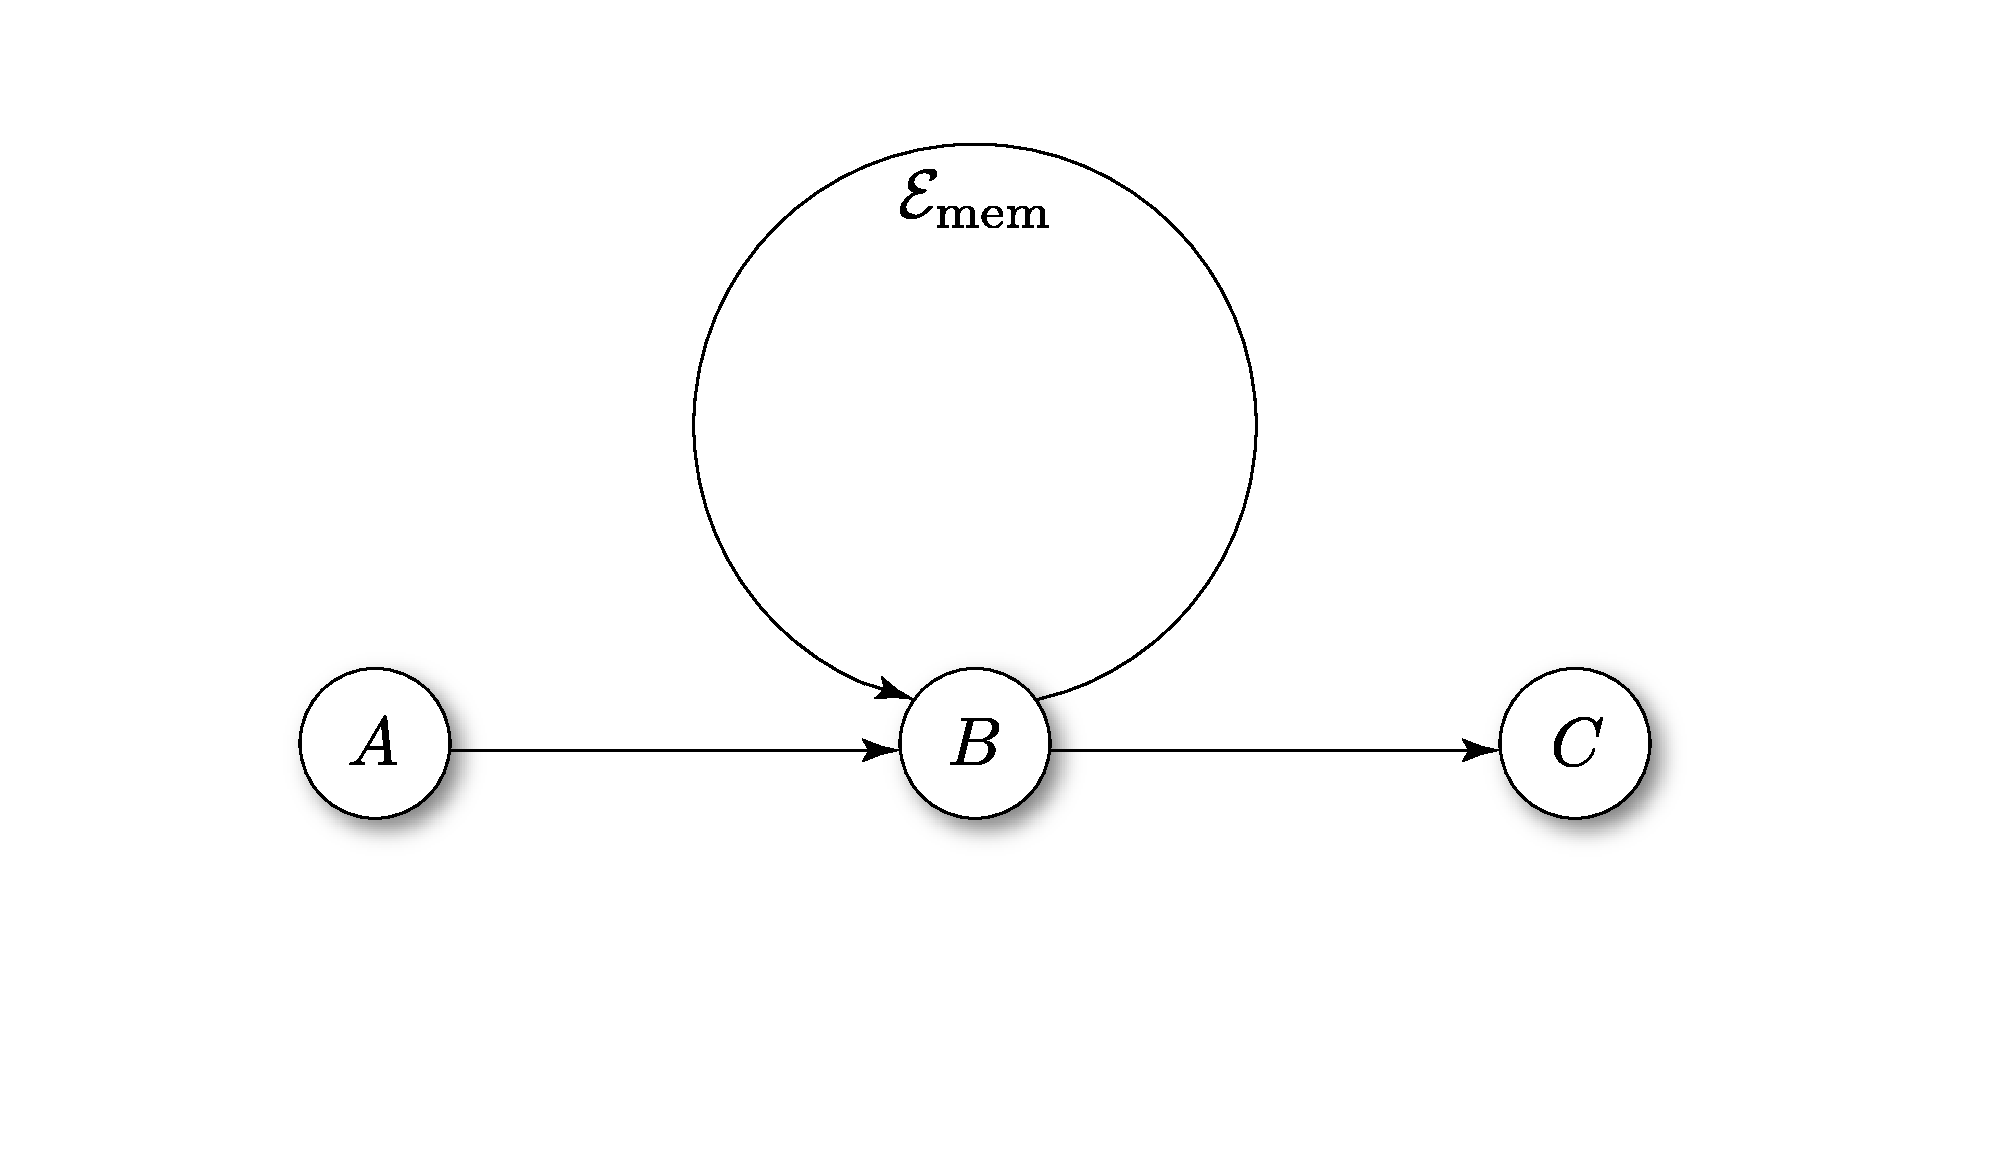
\includegraphics[width=0.7\columnwidth]{memory}
\caption{Simple model for a quantum memory via a self-loop that passes through a memory process, $\mathcal{E}_\mathrm{mem}$. Ideally, $\mathcal{E}_\mathrm{mem}$ does not affect any of the costs or attributes of states passing through the link, except for the latency cost, which is incremented according to the duration of the memory.} \label{fig:memory}
\end{figure}

\subsection{Elementary Protocols}

Building upon the above building blocks, we now describe some of the major elementary quantum protocols. All of those discussed here have been subject to extensive experimental investigation and demonstration.

\subsubsection{Entanglement Purification}

Entangled states, most notably Bell- or Einstein-Podolsky-Rosen (EPR)-pairs,
\begin{align} \label{eq:bell_basis}
\ket{\Phi^{\pm}} &= \frac{1}{\sqrt{2}} (\ket{0}_A\ket{0}_B \pm \ket{1}_A\ket{1}_B), \nonumber \\
\ket{\Psi^{\pm}} &= \frac{1}{\sqrt{2}} (\ket{0}_A\ket{1}_B \pm \ket{1}_A\ket{0}_B),
\end{align}
play a central role in many quantum technologies. These maximally entangled states are easily represented optically using polarization encoding of single photons, and can be non-deterministically prepared directly using spontaneous parametric down-conversion (SPDC).

Bell pairs are the basis for building cluster states (see Sec.~\ref{sec:CSQC}), some quantum cryptography protocols (see Sec.~\ref{sec:QKD}), and quantum teleportation, to name just a few applications. Therefore distributing entangled states with the highest entanglement metrics is extremely important.

Suppose Alice and Bob share an entangled pair. Quantum mechanics, specifically the very definition of entanglement itself, prohibits local operations performed by Alice and Bob from increasing the level of entanglement. However, if Alice and Bob share multiple pairs, they can perform an operation known as \emph{entanglement purification}, whereby two lower-fidelity entangled pairs are consumed and projected onto a single entangled pair with higher-fidelity. Such protocols will be extremely useful in protocols where achieving the highest possible degree of entanglement is paramount.

Taking two polarization-encoded photonic Bell pairs, say $\ket{\Psi^+}$ and subjecting them to a dephasing error model yields a mixed state of the form,
\begin{align}
\hat\rho_\mathrm{in} = F\ket{\Psi^+}\bra{\Psi^+} + (1-F)\ket{\Psi^-}\bra{\Psi^-},
\end{align}
where $F$ is the entanglement fidelity, which is a function of the dephasing rate. Note that $\ket{\Psi^+}$ and $\ket{\Psi^-}$ are related by local phase-flip operations ($\hat{Z}$) applied to either qubit.

An linear optics entanglement purification protocol can be simply implemented using two polarizing beamsplitters (PBSs). Alice uses one PBS to interfere the photons from her side of each of the photon pairs, measuring one output only, which implements a Bell projection. Bob does the same on his side. What's left is one photon in Alice's hands and one in Bob's. When successful, they will now be sharing a single entangled pair of higher Bell state fidelity than the two starting states. The protocol is shown in Fig.~\ref{fig:ent_purif_prot}.

\begin{figure}[!htb]
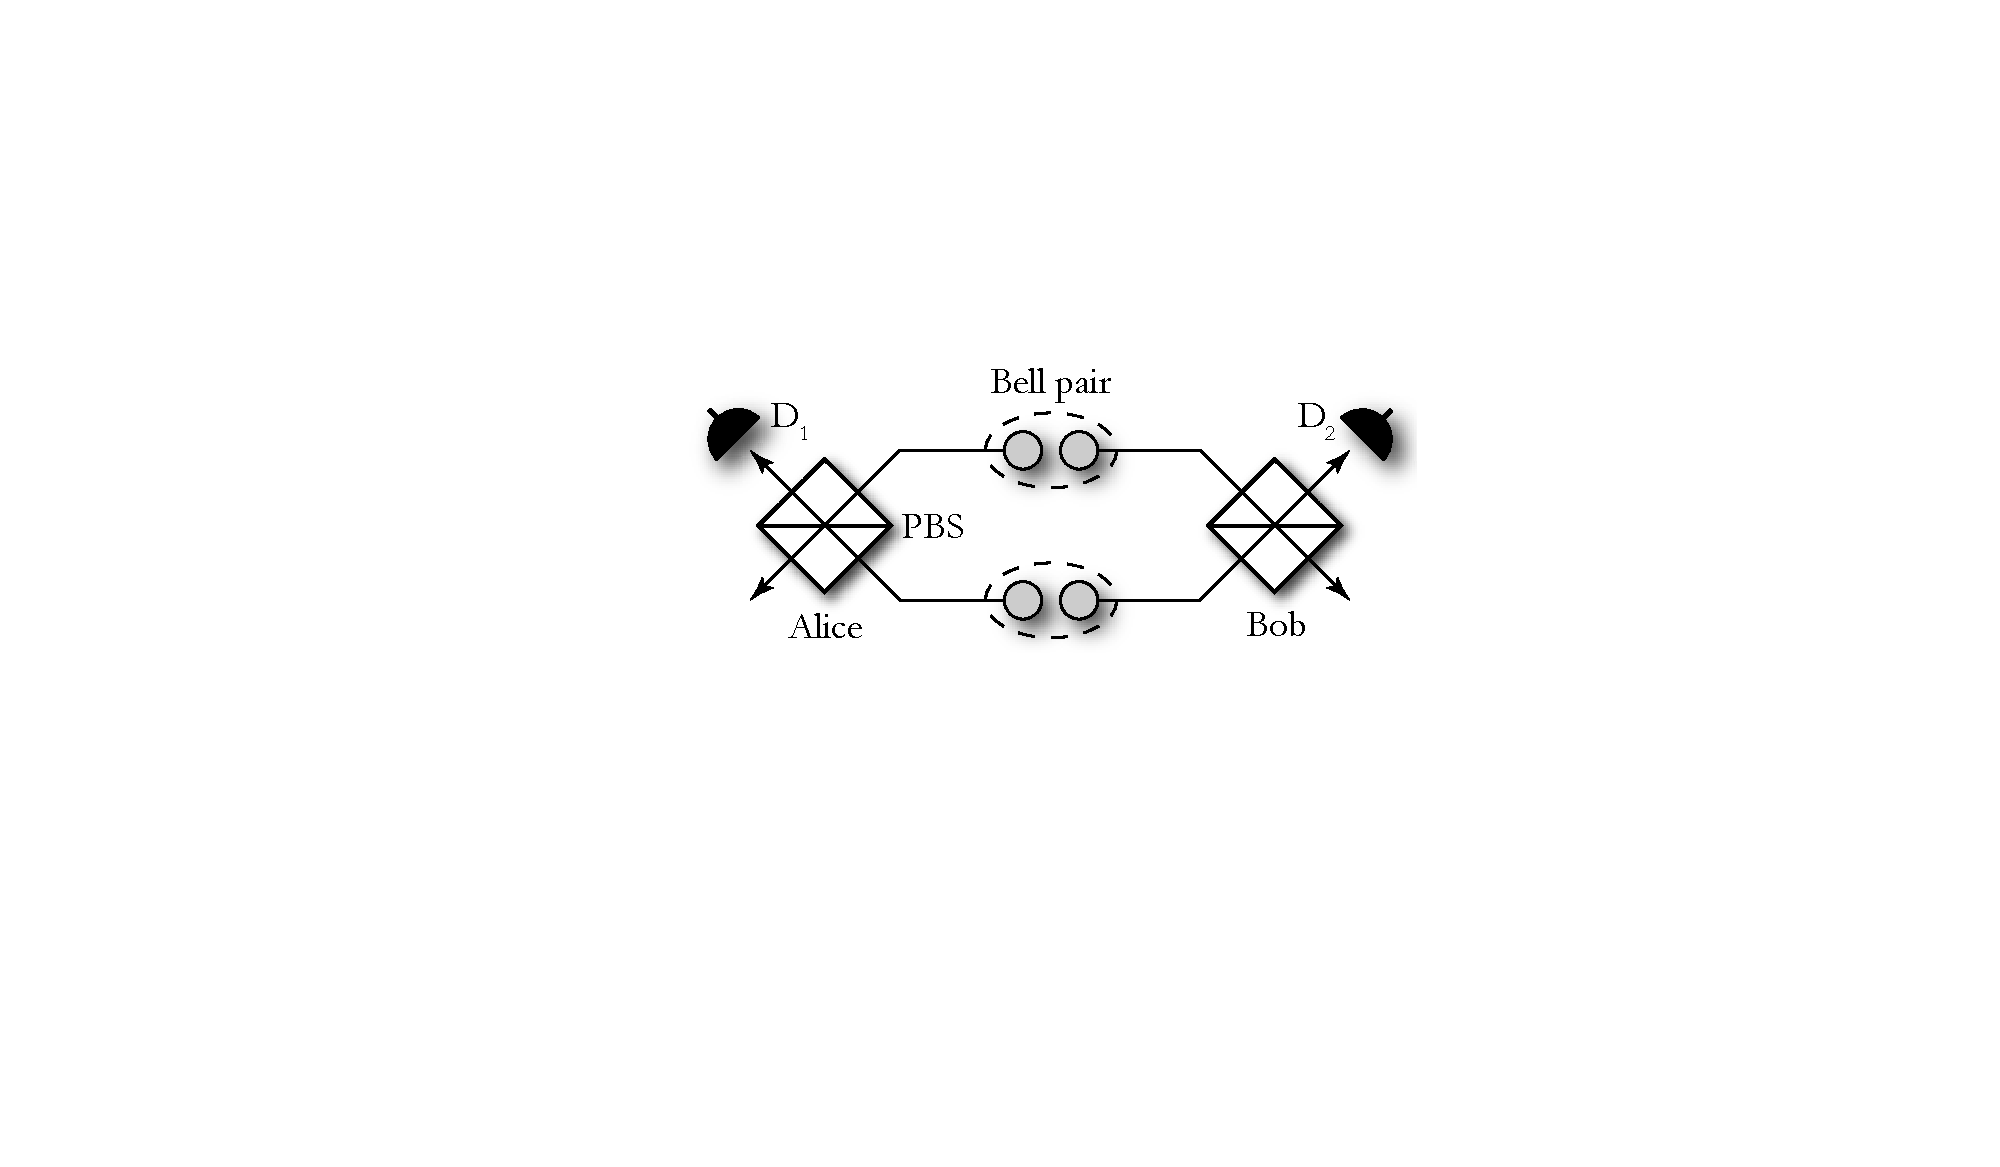
\includegraphics[width=0.9\columnwidth]{ent_purif_prot}
\caption{Elementary entanglement purification using linear optics. Two Bell pairs are distributed between Alice and Bob, each of which has been subject to a dephasing error model. Alice and Bob perform Bell measurements on their two qubits using a polarising beamsplitter (PBS) and polarisation-resolved photodetection ($D_1$ and $D_2$). Upon successful Bell-state projection (Bell measurements are necessarily non-deterministic using linear optics), Alice and Bob will share a single Bell-pair with higher fidelity than the two input pairs.} \label{fig:ent_purif_prot}
\end{figure}

Specifically, the relationship between the input ($F_\mathrm{in}$) and output ($F_\mathrm{out}$) fidelities of the protocol is,
\begin{align}
F_\mathrm{out} = \frac{{F_\mathrm{in}}^2}{{F_\mathrm{in}}^2 + (1-F_\mathrm{in})^2}.
\end{align}
This input/output relationship is shown in Fig.~\ref{fig:ent_purif}.

\begin{figure}[!htb]
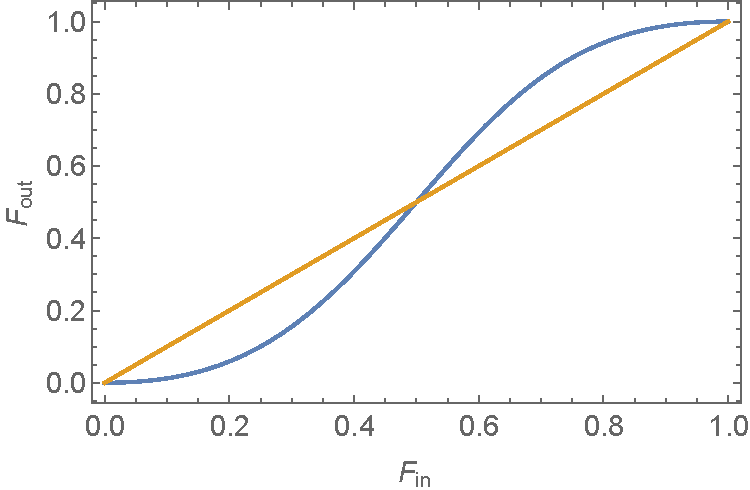
\includegraphics[width=\columnwidth]{ent_purif}
\caption{Entanglement purification of two polarization-encoded, photonic Bell pairs. $F_\mathrm{in}$ ($F_\mathrm{out}$) are the input (output) fidelities of the Bell pairs. The protocol consumes two Bell pairs for every one purified pair. The straight line represents the break-even point in terms of state fidelity, above which the protocol enhances fidelity, and below which reduces it. This places a strict bound on the fidelity of Bell pairs reaching the purifier. This equates to route cost, if measured by the fidelity metric, stipulating network performance requirements. This threshold requirement presents an example of where an {\sc All or Nothing} strategy might be appropriate.} \label{fig:ent_purif}
\end{figure}

Note that there is a break-even point, above which the protocol strictly increases fidelity, and below which strictly decreases it. This occurs at \mbox{$F_\mathrm{in}=1/2$}. Provided pairs can be communicated above this fidelity threshold, bootstrapped application of the protocol could be employed to boost entanglement fidelity asymptotically close to unity (but with exponential resource overhead, since each operation consumes two pairs to produce one). But below this threshold it is impossible to recover any more entanglement than we started with. This provides an example of an application where the protocol being implemented dictates strict requirements on network cost metrics. Specifically, assuming perfect Bell pairs to begin with, the routes by which they are communicated must ensure entanglement fidelities of at least \mbox{$F=1/2$} upon reaching destination. Here a type of {\sc All or Nothing} networking strategy would be applicable -- if the fidelity requirement is not met, the state cannot be purified and might as well be thrown away to make way for other traffic.

A theoretical analysis of this protocol has been performed, accounting for mode-mismatch in the protocol \cite{bib:RohdeOptEntPur06}, where it was found than mode-mismatch shifts the break-even point upwards, and lowers the maximum value of $F_\mathrm{out}$ -- with more mode-mismatch, a higher starting fidelity is required to break even, and we achieve a lower output fidelity. In this case, a cost function that combines the dephasing and mode-mismatch metrics of the network will be required.

\subsubsection{Quantum Teleportation}

Quantum teleportation is an essential ingredient in many higher-level protocols. It forms the basis of cluster state quantum computing (see Sec.~\ref{sec:CSQC}), some QEC codes, the KLM linear optics quantum computing scheme (see Sec.~\ref{sec:KLM_univ}), and can act as a mediator for long-range transmission of quantum states, amongst others.

In the standard teleportation protocol, Alice begins with a single qubit,
\begin{align}
\ket\phi = \alpha\ket{0} +\beta\ket{1},
\end{align}
which she would like to teleport to Bob. Importantly, no quantum communication between the two is allowed, since obviously this would make the problem trivial. However, classical communication is allowed (and turns out to be necessary), and furthermore they share an entangled Bell pair. Thus, Alice begins with two qubits, and Bob begins with one -- his half of the entangled pair onto which Alice's state ought to be teleported. The initial state is therefore,
\begin{align}
\ket\psi_\mathrm{in} &= \ket{\phi}_{A_1} \ket{\Psi^+}_{A_2,B} \nonumber \\
&= \frac{1}{\sqrt{2}} (\alpha\ket{0}_{A_1}+\beta\ket{1}_{A_1}) (\ket{0}_{A_2}\ket{1}_B + \ket{1}_{A_2}\ket{0}_B).
\end{align}

The first step of the protocol is for Alice to perform a two-qubit entangling measurement on her two qubits, projecting onto the Bell basis (Eq.~\ref{eq:bell_basis}). She obtains one of four measurement outcomes. For illustration, suppose she measures the $\ket{\Psi^+}$ outcome. Then the projected state is,
\begin{align}
\ket\psi_\mathrm{proj}^{\Psi^+} &= \bra{\Psi^+}_{A_1,A_2} \ket\psi_\mathrm{in} \nonumber \\
&= \frac{1}{\sqrt{2}} \bra{\Psi^+}_{A_1,A_2}\ket\psi_{A_1}(\ket{0}_{A_2}\ket{1}_B + \ket{1}_{A_2}\ket{0}_B) \nonumber \\
&= \frac{1}{2} (\bra{0}_{A_1}\bra{1}_{A_2} + \bra{1}_{A_1}\bra{0}_{A_2}) \nonumber \\
&\cdot (\alpha\ket{0}_{A_1}+\beta\ket{1}_{A_1})(\ket{0}_{A_2}\ket{1}_B + \ket{1}_{A_2}\ket{0}_B) \nonumber \\
&= \frac{1}{2} (\alpha \ket{0}_B + \beta \ket{1}_B)\nonumber \\
&= \frac{1}{2} \ket\phi_B,
\end{align}
which is Alice's initial state. For all four possible Bell measurement outcomes we have,
\begin{align}
\ket\psi_\mathrm{proj}^{\Psi^+} &= \frac{1}{2} (\alpha \ket{0}_B + \beta \ket{1}_B) \nonumber \\
&= \ket\phi_B, \nonumber \\
\ket\psi_\mathrm{proj}^{\Psi^-} &= \frac{1}{2} (\alpha \ket{0}_B - \beta \ket{1}_B) \nonumber \\
&= \frac{1}{2} \hat{Z}\ket\phi_B, \nonumber \\
\ket\psi_\mathrm{proj}^{\Phi^+} &= \frac{1}{2} (\alpha \ket{1}_B + \beta \ket{0}_B) \nonumber \\
&= \frac{1}{2} \hat{X} \ket\phi_B, \nonumber \\
\ket\psi_\mathrm{proj}^{\Phi^-} &= \frac{1}{2} (\alpha \ket{1}_B - \beta \ket{0}_B) \nonumber \\
&= \frac{1}{2} \hat{X}\hat{Z}\ket\phi_B,
\end{align}
which are all locally equivalent to $\ket\phi$ under Pauli gates, and can be corrected by Bob, given communication of the classical Bell measurement outcome provided by Alice. The protocol is shown in Fig.~\ref{fig:teleport}.

\begin{figure}[!htb]
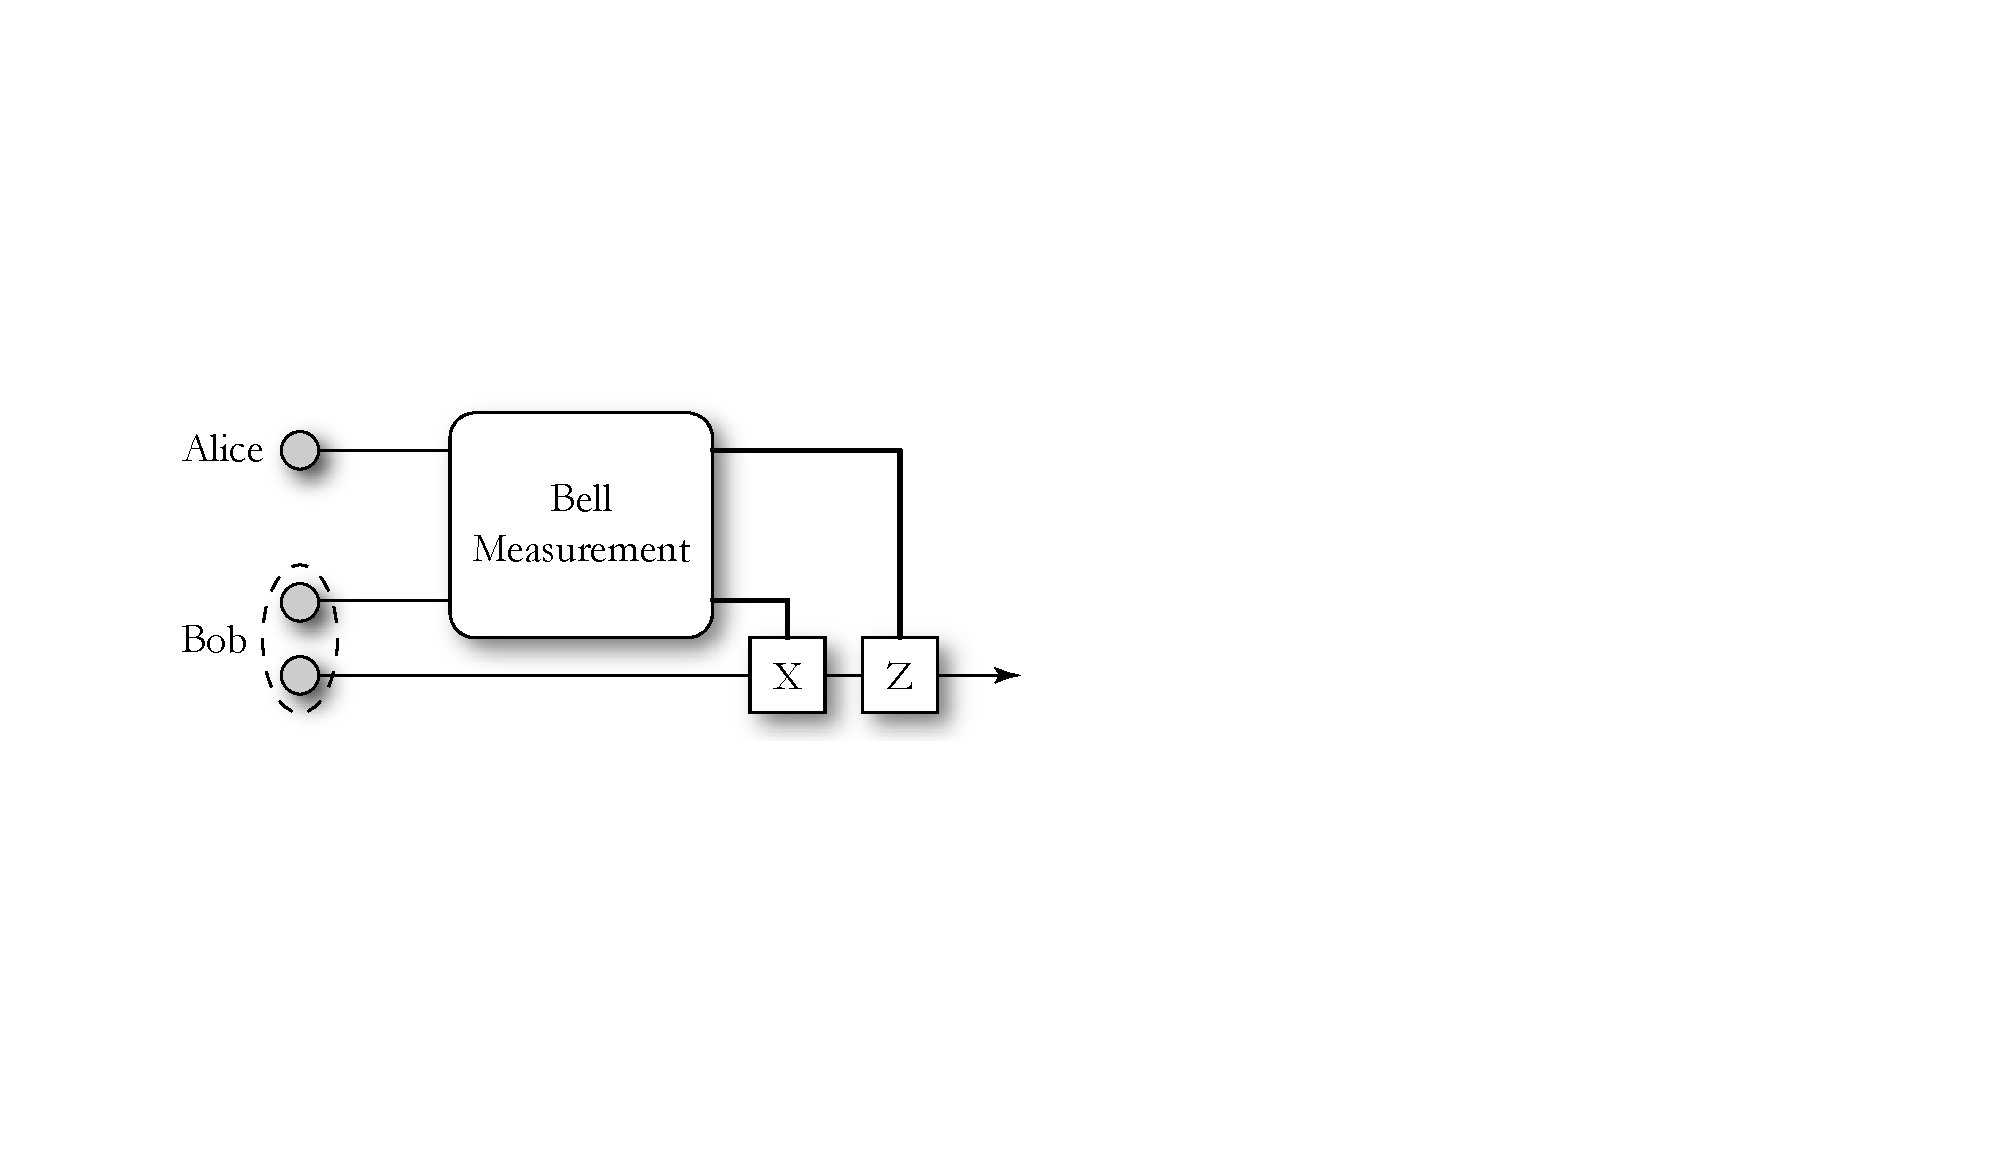
\includegraphics[width=0.9\columnwidth]{teleportation}
\caption{Teleportation of a single qubit. Alice holds a single qubit (top grey circle), which she would like to teleport to Bob. Bob holds a Bell pair (dotted ellipse), and shares one of its qubits with Alice, who performs a Bell measurement on in and her qubit. Depending on the measurement outcome, one of four combinations of local operations is applied to Bob's qubit, after which he has Alice's qubit.} \label{fig:teleport}
\end{figure}

In general, the protocol is deterministic, although in linear optics it has at most a 50\% success probability, since deterministic Bell measurements are not possible in linear optics -- no passive linear optics device can distinguish between more than two of the Bell states.

The question now is what error metrics apply and how do they accumulate in the teleportation protocol. The answer is straightforward -- the final teleported qubit accumulates all local Pauli errors (e.g dephasing or depolarization) associated with Alice's input state as well as any that acted upon the shared Bell pair. That is, the errors get teleported along with the state being teleported, plus any errors on the Bell pair.

In the case of loss, loss of either of Alice's qubits will immediately be detected when she performs her Bell measurement. Thus, loss becomes a located error, and the knowledge of the error allows the associated packet to be discarded and the sender and recipient notified. On the other hand, loss on Bob's qubit will behave no differently than loss acting on an ordinary qubit channel.

Thus, in terms of Pauli errors, no special treatment is required by the QTCP protocol -- it is almost as if the teleportation protocol weren't there. And in terms of loss, the Bell state projection diagnoses lost qubits, allowing appropriate action to be taken, which is actually better than if the error were undiagnosed.

The total resources required to teleport a single qubit are: the qubit to be teleported, a single Bell pair, a two-qubit measurement in the Bell basis, and the transmission of two classical bits. This is more costly than sending the qubit using a direct link, but may be the only approach if a direct link is not available.

\subsubsection{Entanglement Swapping \& Quantum Repeaters} \label{sec:repeater}

The obvious approach to sending a qubit from Alice to Bob is to send a qubit from Alice to Bob. However, over long distances this may accrue impractical error rates, particularly losses. The other alternative is to employ the quantum teleportation protocol to teleport the state between the two parties. However, this requires that Alice and Bob first share an entangled Bell pair, which must itself be distributed across the same distances. \emph{Quantum repeaters} are devices that allow entanglement to be shared between distant nodes using a bootstrapped \emph{entanglement swapping} protocol. Entanglement swapping is the process of taking two Bell pairs, one held by each party, and swapping the entanglement between them such that the two parties share an entangled state. This procedure can be bootstrapped to progressively swap the entanglement over longer and longer distances.

Specifically, suppose Alice and Bob possess the entangled states $\ket{\Phi^+}_{A_1,A_2}$ and $\ket{\Phi^+}_{B_1,B_2}$. That is, their entanglement is held locally and none is shared between them. Now let each of them transmit one of their qubits to a node that performs and entangling Bell measurement on them. Now Alice and Bob will share the two-qubit state $\ket{\Phi^+}_{A,B}$ -- the entanglement has been swapped from one set of qubits to another. For example, for the input state,
\begin{align}
\ket\psi_\mathrm{in} = \ket{\Phi^+}_{A_1,A_2} \ket{\Phi^+}_{B_1,B_2},
\end{align}
the state following a Bell projection onto $\ket{\Phi^+}_{A_1,B_1}$ is,
\begin{align}
\bra{\Phi^+}_{A_1,B_1} \ket\psi_\mathrm{in} = \ket{\Phi^+}_{A_2,B_2}.
\end{align}

Now if instead of Alice and Bob we have a long chain of these operations in series, then the entanglement can be swapped across the entire length of the chain, enabling the preparation of end-to-end entangled pairs, which can be employed for state teleportation. The protocol is shown in Fig.~\ref{fig:ent_swap}.

\begin{figure}[!htb]
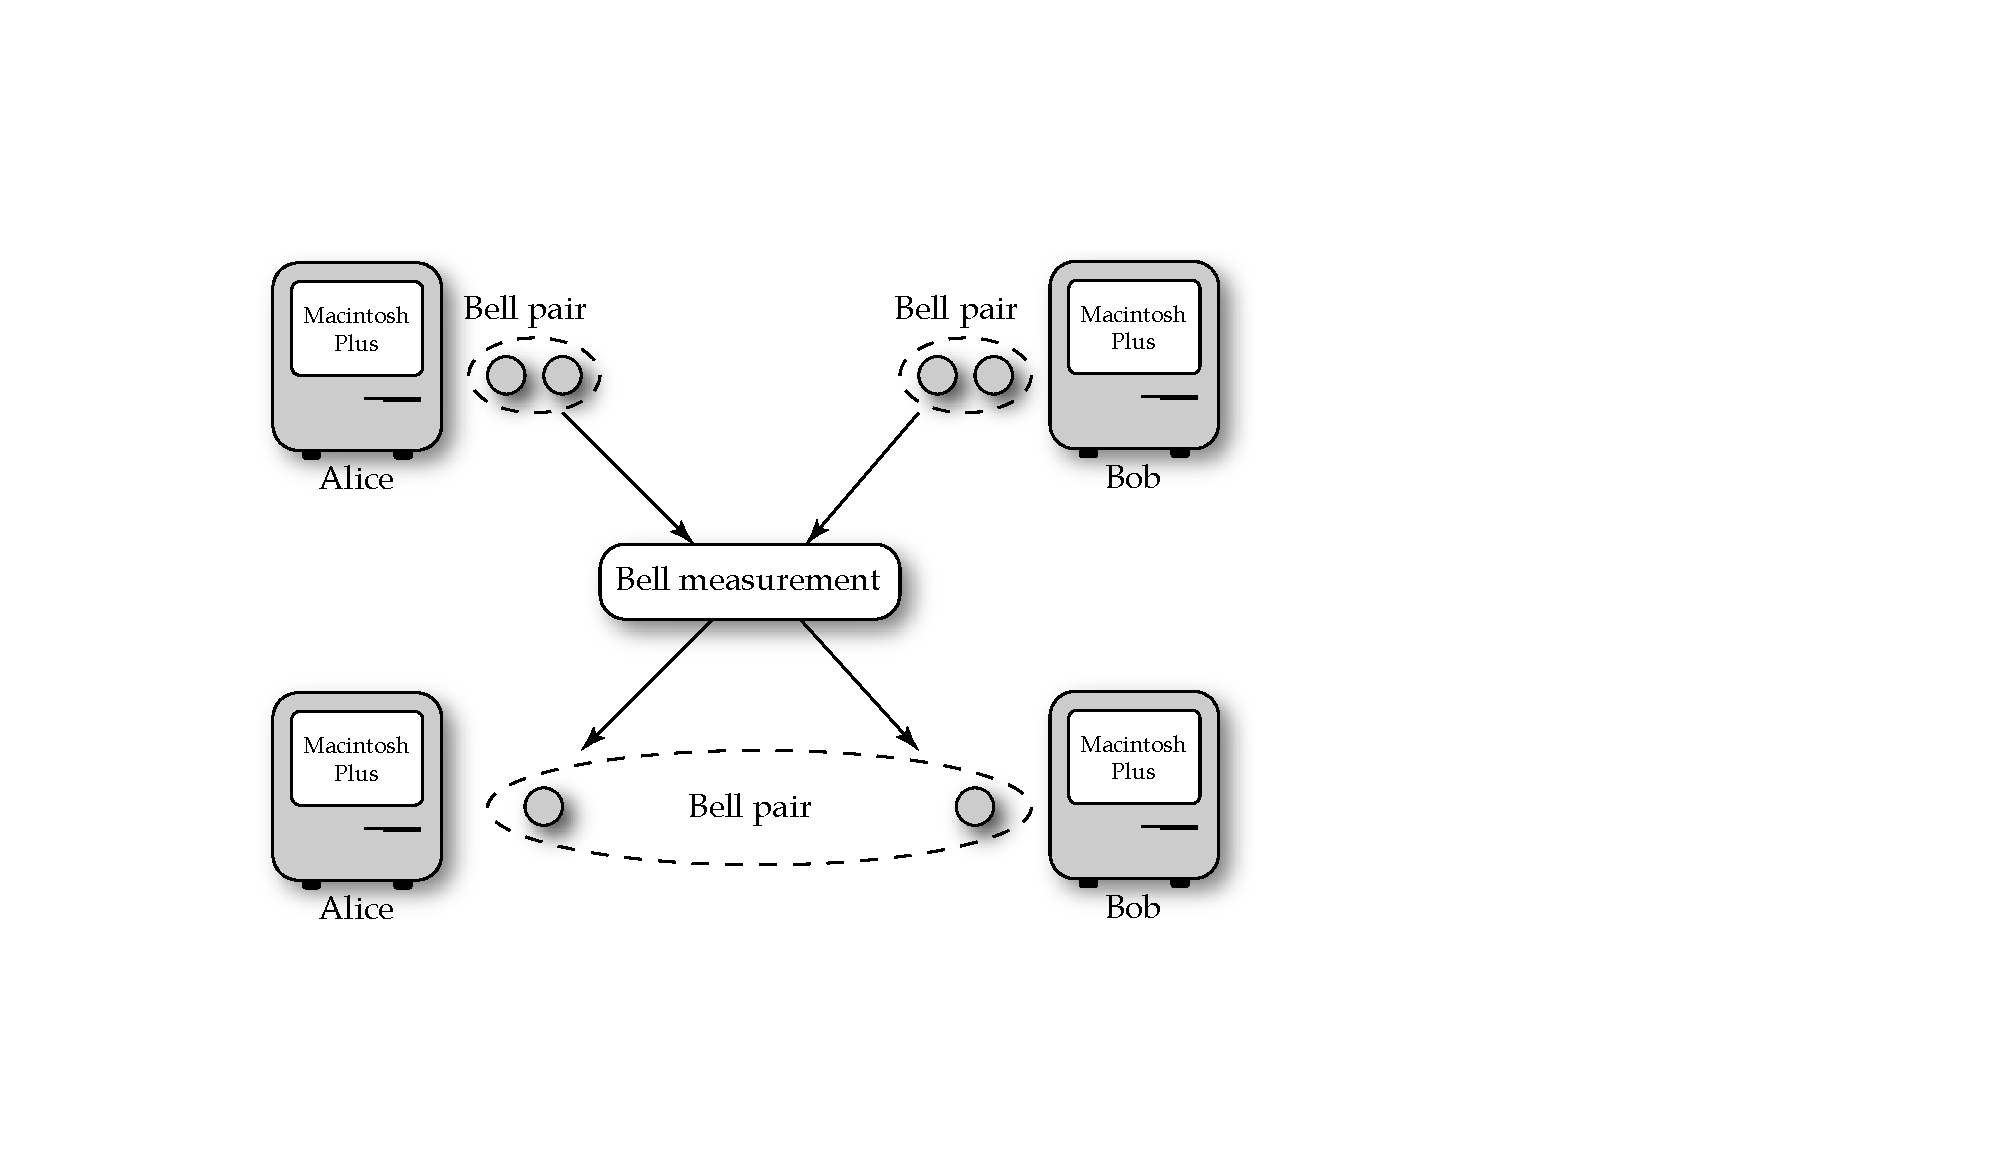
\includegraphics[width=\columnwidth]{ent_swap}
\caption{Entanglement swapping between two nodes. Each node initially holds a Bell pair (dotted ellipses) comprising two qubits (grey circles). One qubit from each pair is sent to repeater between them, which measures them in the Bell basis. After local unitary corrections, the two nodes share an entangled pair.} \label{fig:ent_swap}
\end{figure}

The advantage to this approach is that the range of each repeater can be much smaller than the entire length of the channel, easing constraints imposed by errors, notably loss. Furthermore, the entanglement swapping needn't be actually performed in any chronologically linear sequence. The operations could be arbitrarily ordered. Thus, if some segments are detected as failing (e.g qubits are lost), just those segments can be performed again without requiring the entire protocol to start from scratch, unlike the na{\" i}ve direct communication technique.
This `divide and conquer' approach can drastically improve performance of the network in terms of channel capacity, improving the exponential dependence of loss on distance.

Because the protocol is constructed entirely on top of many instances of the teleportation protocol, it inherent all the same error propagation characteristics as for teleportation discussed previously.

\subsubsection{Optical Interfacing}

\comment{TO DO}

\subsubsection{Quantum Memory}

A key requirement in large-scale quantum networks will be the ability to store qubits. This will be required when, for example, quantum data packets reach a network bottleneck, and face one of two options: wait, or be discarded. As discussed earlier, discarding quantum packets is often a highly undesirable enterprise, as they often cannot be easily recreated.

Storing photons directly is challenging owing to their travelling nature, and ease with which they can be absorbed and lost. One approach has been to use optical cavities to trap photons, but storage times and efficiencies using this technique remain impractically low.

A more plausible approach is to convert optical qubits to matter qubits with long lifetimes. Some matter-based qubits are being demonstrated with very long decoherence times. For example, atomic ensemble qubits have been demonstrated with decoherence times on the order of hundreds of milliseconds \comment{Check this!} \cite{???}, certainly long enough to wait out a typical network bottleneck.

This effectively reduces the problem of optical quantum memory to that of optical interfacing between light-matter systems, as discussed in the previous section, and all the previously discussed issues surrounding optical interfacing apply as described.

However, in addition to this, the quantum memory will of course accumulate additional costs associated with the idle storage time. This could be in the form of any of the usual error models applying to the matter qubit in question. In terms of our graph-theoretic description, memory can be modeled as self-loops at nodes, where the quantum process of the looped link is that of a single unit of time in the quantum memory. The remainder of the QTCP framework remains unchanged, although it must be ensured that the network strategy algorithms function correctly with self-loops.

\subsubsection{Quantum Key Distribution (QKD)} \label{sec:QKD}

\comment{Show technical details}

Aside from quantum computing, a central use for quantum technologies is in cryptography \cite{bib:Gisin02}. There is only a single provably secure encryption protocol, the \emph{one-time-pad}. This protocol requires Alice and Bob to share a random bit-string as long as the message being communicated between them. This reduces the problem of perfect secrecy of arbitrary messages to secrecy of shared randomness. QKD protocols enable this by providing a shared source of randomness between Alice and Bob, where any intercept-resent attack may be detected, guaranteed by the laws of quantum physics.

The two original QKD protocols, known as the \emph{BB84 protocol}) \cite{bib:BennetBrassard84}, and \emph{Ekert 91 protocol} \cite{bib:Ekert91}, are based on polarisation encoding in photons. BB84 requires only the transmission of a sequence of single photons, polarisation encoded with random data. Ekert 91, on the other hand, requires a server that distributes entangled Bell pairs between Alice and Bob. Since, numerous other protocols for QKD have been proposed, for example, using continuous variable states.

It is easy to see the utility of quantum networks in enabling commodity deployment of QKD -- users desire to communicate photons across long-range ad hoc networks, with low loss, so as to maximise bit-rates, and minimising costs in, for example, fidelity, entanglement, and purity. A global quantum internet would allow quantum cryptography to truly supersede classical cryptography, bypassing the vulnerabilities faced by classical cryptography in the quantum computing era.

Unlike quantum computing, QKD is at the stage of commercial viability, and several vendors offer off-the-shelf plug-and-play QKD systems. Thus, a quantum internet with low cost metrics would already find substantial utility with today's technology. Currently, great progress in being made in the implementation of QKD in fibre \cite{???}, over free space \cite{bib:Buttler00}, and even over intercontinental satellite uplinks \cite{JWP}. It seems extremely likely that some government agencies would be rolling out QKD systems \cite{bib:Secret}, especially in light of the paranoia surrounding quantum codebreaking.

\subsection{Cloud Quantum Computing} \label{sec:cloud}

From the perspective of quantum computing, by far the most pressing goal for quantum networking is to facilitate \emph{cloud quantum computing}, whereby computations can be performed over a network via a client/server model. This will be of immense importance economically, allowing the very expensive quantum computers to be accessible to end users, who would be unable to purchase them themselves. This economic model is critical to the widespread adoption of quantum computation.

There are several protocols necessary to facilitate cloud quantum computing. First of all, we must have a means by which to remotely process data prepared by a host on a server(s). At the most basic level, this simply involves communicating quantum and/or classical data from a client to a single server for processing, which returns quantum or classical information to the client. In the most general case, a computation may be processed by multiple servers, each responsible for a different part of the computation -- \emph{distributed quantum computation}. Many real-world applications for quantum computing will involve sensitive data, in terms of both the information being processed and the algorithms being employed. This necessitates encryption allowing computations to be performed securely over a network, such that intercept-resend attacks are unable to infer the client's data. These form the basic building blocks from which a secure cloud-based model for quantum computing may be constructed, and economic models based on the outsourcing of computations may emerge.

\subsubsection{Single Client, Single Server}

Most simply, an outsourced computation involves Alice preparing either a quantum or classical input state, which she would like processed on Bob's computer. Bob performs the computation and returns either a quantum or classical state to Alice.

The algorithm, which Bob implements, could either be stipulated by Alice, in which case she is purely licensing Bob's hardware, or by Bob, in which case she is licensing his hardware and software. In the case of classical input and classical output, such an outsourced computation is trivial from a networking perspective, requiring no usage of the quantum network whatsoever. In the case of quantum input and/or output data, the quantum network will be required.

Despite the model being very simple, there may still be stringent requirements on the costs in the network. When the result of the computation is returned to Alice, there may be fidelity requirements. An approximate solution to a problem, or a computation with any logical errors whatsoever, may be useless, particularly for algorithms, which are not efficiently verifiable. For example, if Alice is attempting to factorise a large number using Shor's algorithm \cite{bib:ShorFactor}, a number of incorrect digits may make the the correct solution realistically impossible to determine. Or if a large satisfiability problem is being solved, almost any classical bit-flip errors will invalidate the result, requiring additional computation by Alice to resolve.

In the case of classical communication of input and output data, we can reasonably assume error-free communication, owing to its digital nature. However, in the case of quantum communication it is inevitable that at least some degree of noise will be present. Depending on the application, this may require the client and host to jointly implement a distributed implementation of Quantum Error Correction (QEC) \cite{bib:Shor95, bib:CalderbankShor96, bib:NielsenChuang00}, whereby Alice and Bob communicate encoded states with one another, to which syndrome measurement and error correction are applied upon receipt. This will necessitate a limited amount of quantum processing to be directly available to Alice. In the case where she is completely starved of any quantum processing resources whatsoever, this may be a limiting factor. Otherwise, this type of cooperative QEC may be plausible.

\subsubsection{Distributed Computation} \label{sec:dist_QC}

The elementary model described above is very limited, as many realistic data processing applications will require multiple stages of computations to be performed, potentially by different hosts. For example, a client may need data processed using multiple proprietary algorithms owned by different hosts, and the processing will need to be distributed across the network.

There are two main models for how a distributed computation may proceed -- in \emph{parallel}, or in \emph{series} -- whereby sub-algorithms are performed either side-by-side simultaneously, or one after another progressively. The two models are illustrated in Fig.~\ref{fig:distributed}.

\begin{figure}[!htb]
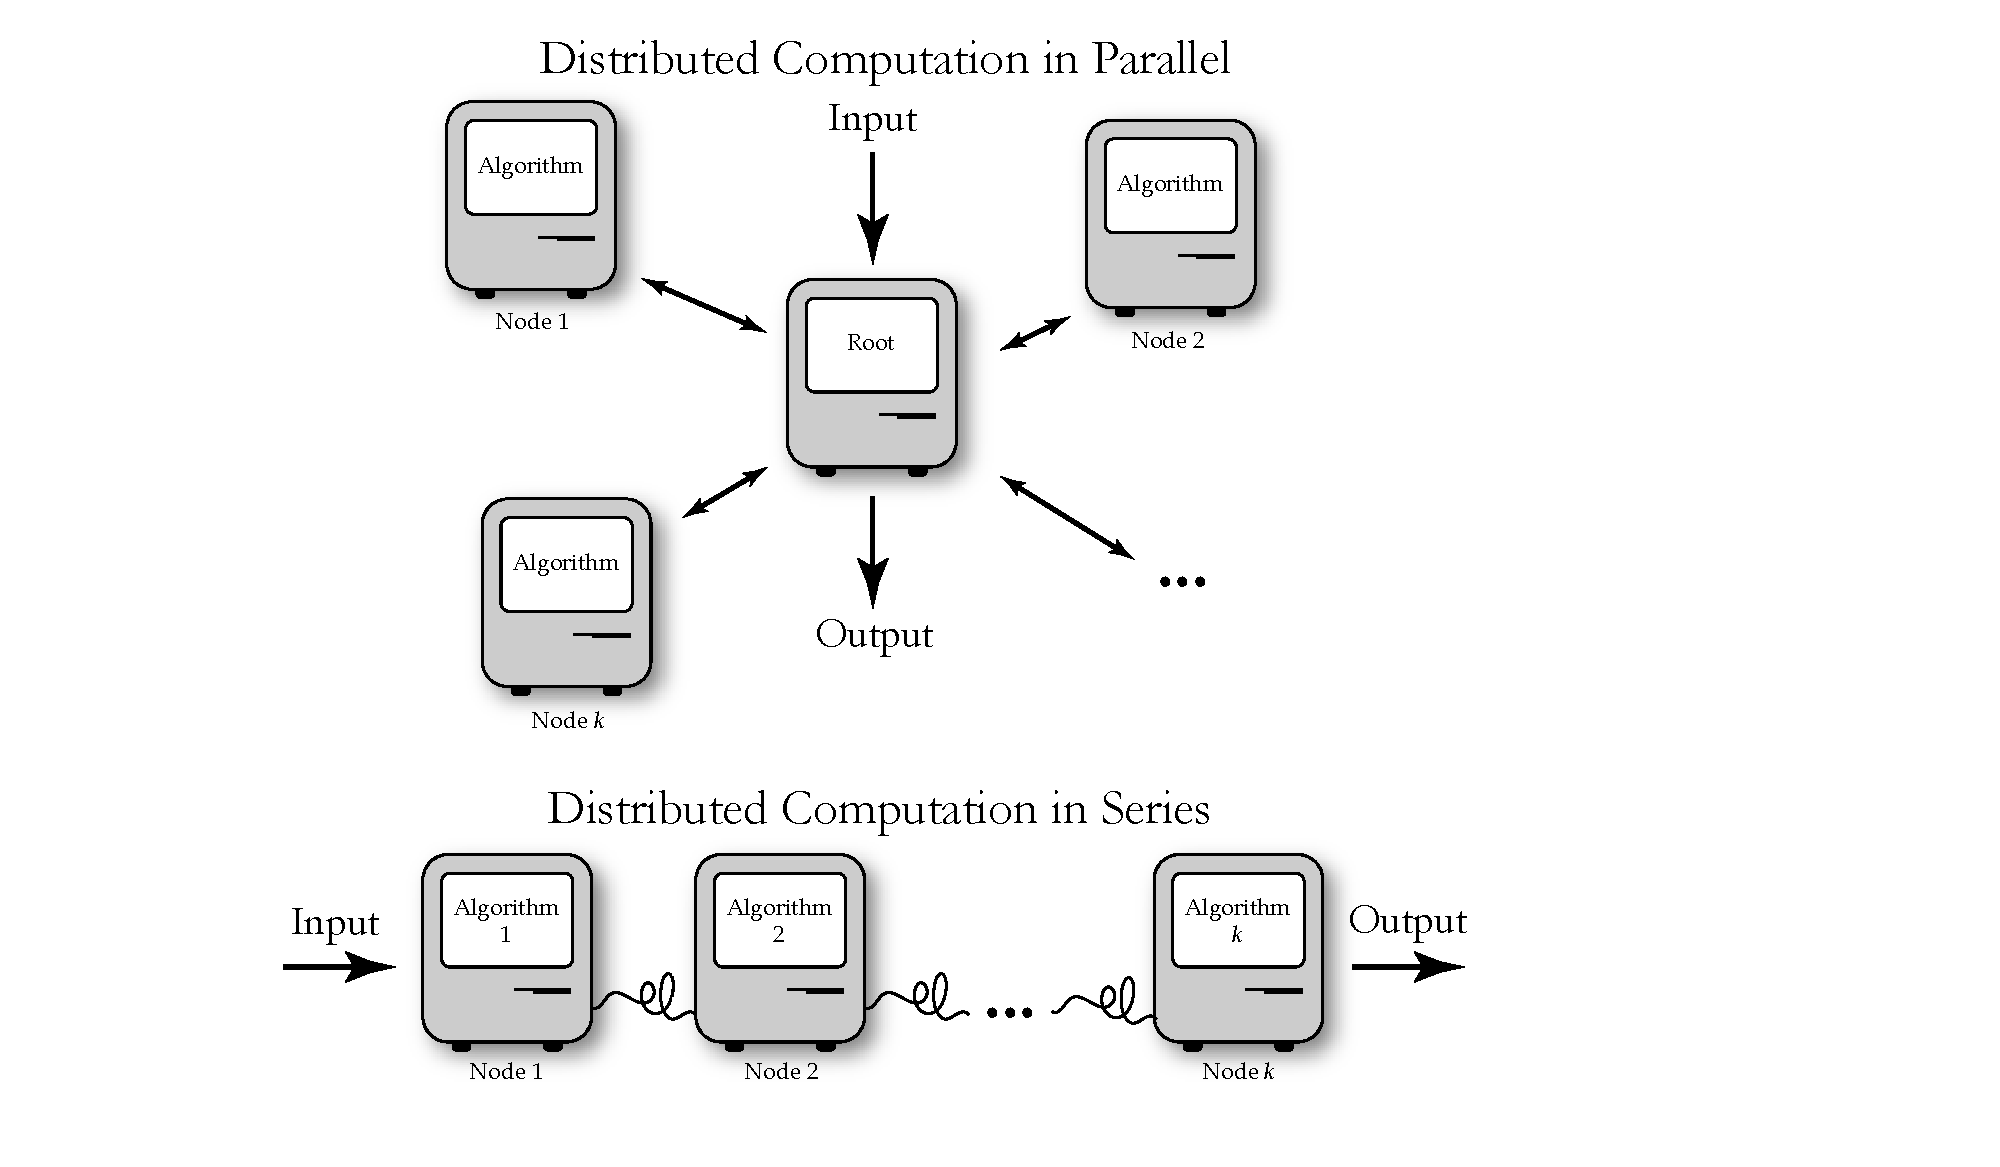
\includegraphics[width=\columnwidth]{distributed}
\caption{Models for distributed computation in parallel and in series. In parallel a root node oversees the total computation, delegating tasks to child nodes, which process data independently of one another. In series the nodes sequentially process data in a pipeline of algorithmic stages.} \label{fig:distributed}
\end{figure}

Classical parallel processing typically involves a root node, which delegates tasks to be performed in parallel by a number of child nodes, and the results returned to the root node, which potentially applies an algorithm to merge the set of results, before returning a final result to the client. Models such as Google's {\sc MapReduce} protocol \cite{bib:MapReduce} are built on this idea.

In classical computing, parallel processing is widely employed to shorten algorithmic runtimes. However, the increase in clock-cycles scales only linearly with the number of nodes in the network: $k$-fold parallelization yields a \mbox{$\sim k$}-fold speedup. For time-critical applications, such a linear improvement may be already highly beneficial, albeit costly. The attractive feature of quantum computing, however, is the potentially exponential improvement in algorithmic performance of certain tasks over their classical counterparts. This exponential relationship implies that parallelization no longer has a simple linear tradeoff.

Let $t_c$ be the time required by a classical algorithm to solve a given problem, and $t_q$ the time required to solve the same problem using a quantum algorithm. In the case of algorithms exhibiting exponential quantum speedup, we will have,
\begin{align}
t_c = \mathrm{exp}(t_q).
\end{align}
If we now employ $k$-fold parallelization in the quantum scenario, the equivalent classical processing time is,
\begin{align}
t_c' &= \mathrm{exp}(t_q k) \nonumber \\
&= \mathrm{exp}(t_q)^{k} \nonumber \\
&= {t_c}^{k}.
\end{align}
Thus, $k$-fold quantum parallelization corresponds to a $k$th-order exponential enhancement in the equivalent classical processing time, which scales much more favourably than the linear $k$-fold enhancement offered by classical parallelization.

The alternate scenario is in-series distributed computation, in which a computation proceeds through a pipeline of different stages, potentially performed by different hosts. This model allows a complex algorithm comprising smaller sub-algorithms, each of which may be proprietary with different owners, to be delegated across the network. The different stages may communicate classical and/or quantum data. As with the simple single-host model, if the different stages of the processing pipeline are sharing quantum data, distributed QEC will generally be necessary to protect the computation. This necessarily introduces an (efficient) overhead in the number of physical qubits being communicated across the network, introducing additional bandwidth costs, which must be accommodated for in networking strategies.

\subsubsection{Encryption} \label{sec:homo_blind}

Extremely important to many high-performance data-processing applications is security, as proprietary or sensitive data may be being dealt with. To address this, two models for outsourced quantum computation exist for addressing this -- \emph{homomorphic encryption} \cite{gentry2009fully, van2010fully} and \emph{blind quantum computation} \cite{bib:blind2, bib:blind3, bib:blind1, PhysRevLett.108.200502, bib:Morimae3486, bib:Morimae5460, bib:Morimae3966}.

In both cases, Alice has secret data, and wishes to not only ensure that an interceptor is unable to read it, but that the server performing the computation isn't able to either. That is, she wishes the data to be processed in encrypted form, without first requiring decryption.

The difference between the two protocols lies in the treatment of algorithms. In homomorphic encryption, Alice provides only the data, whereas Bob provides the processing and the algorithm it implements (which he would also like to keep to himself). In blind computing, Alice provides both the algorithm \emph{and} the data, and wishes \emph{both} to remain secret. Both of these protocols seem like very challenging goals, yet significant developments have been made on both fronts. Classical homomorphic encryption has only been described very recently \cite{bib:gentry2009fully, bib:van2010fully}.

In the usual circuit model, blind quantum computation has been shown to be viable, and optimal bounds derived. Similarly, such protocols have been described \cite{homoCS} in the cluster state model (see Sec.~\ref{sec:CSQC}). For universal computation, such protocols necessarily require classical interaction between the client and host. However, it was shown that in some restricted (i.e non-universal) models for optical quantum computation, specifically {\sc BosonSampling} and quantum walks, non-interactive homomorphic encryption may be implemented almost optimally (see Sec.~\ref{sec:BS}).

These encryption protocols induce a resource overhead in circuit size and number of qubits involved in the computation, with efficient scaling. They deliver information-theoretically secure data-hiding, enabling trustworthy outsourced processing of encrypted data, independent of the attack.

\subsubsection{Cluster States} \label{sec:CSQC}

The \emph{circuit model} is the conventional approach for expressing quantum algorithms. However, the \emph{cluster state model} for quantum computation \cite{bib:Raussendorf01, bib:Raussendorf03, bib:Nielsen06} (also referred to as the \emph{one-way}, \emph{measurement-based}, or \emph{graph state} models for quantum computation) is an extremely powerful, yet conceptually distinct paradigm, that warrants treatment of its own, owing to its significant distinction from the more familiar circuit model.

In the cluster state model, we begin by preparing a particular, highly-entangled state, called a \emph{cluster state} or \emph{graph state}. The state is associated with a graph of some topology, although rectangular lattice graphs are usually considered as they are sufficient for universal quantum computation. 

In the graph, vertices represent qubits initialised into the \mbox{$\ket{+}=(\ket{0}+\ket{1})/\sqrt{2}$} state, and edges represent the application of maximally entangling controlled-phase (CZ) gates between vertices, given by \mbox{$\hat{U}_\mathrm{CZ}=\mathrm{diag}(1,1,1,-1)$}. An example is presented in Fig.~\ref{fig:cluster_state}. Cluster states are easily encoded optically using photonic polarisation encoding, and therefore readily lend themselves to optical networking.

\begin{figure}[!htb]
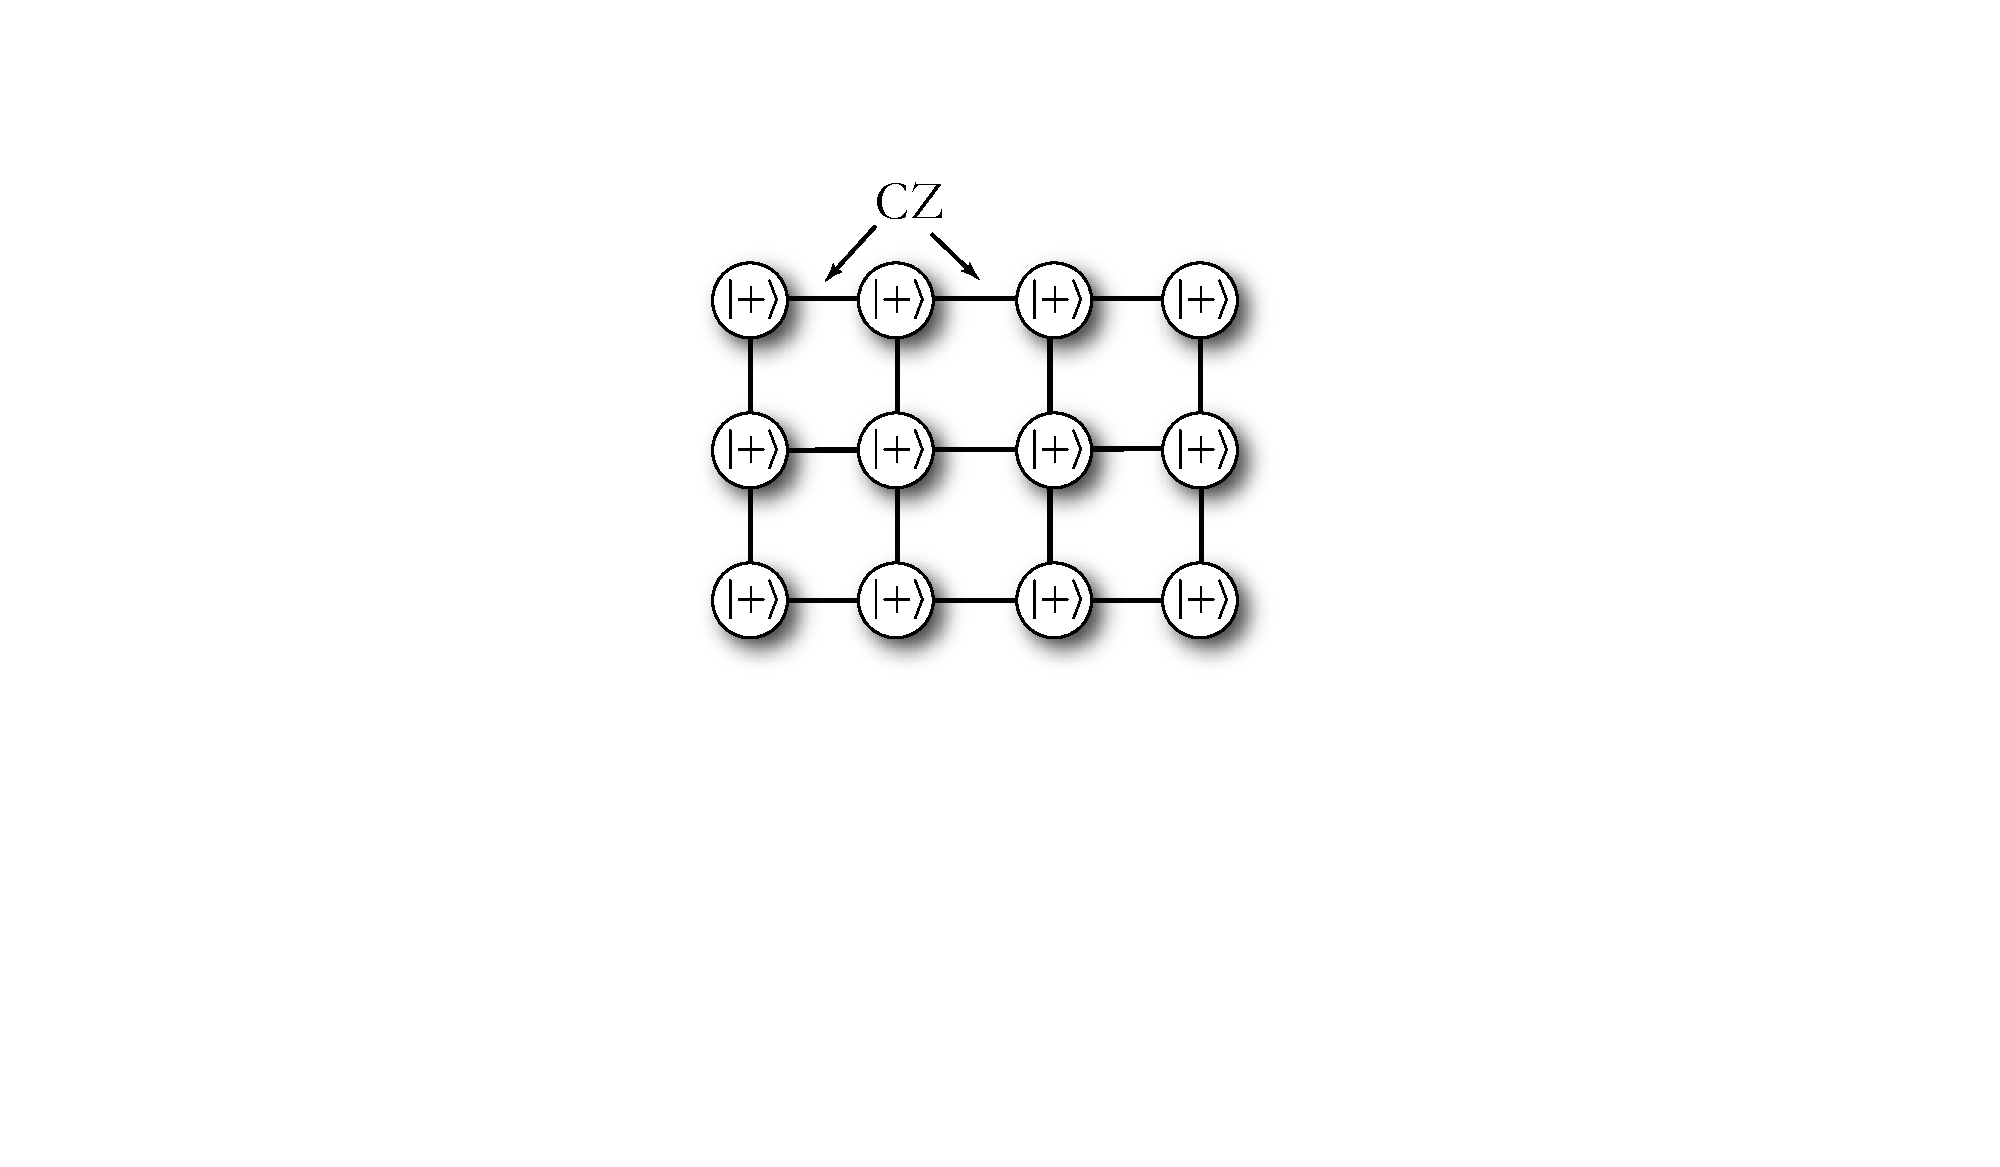
\includegraphics[width=0.7\columnwidth]{cluster_state}
\caption{Example of a \mbox{$4\times 3$} rectangular lattice cluster state. Each vertex in the graph represents a qubit initialised as \mbox{$\ket{+}=(\ket{0}+\ket{1})/\sqrt{2}$}. Edges represent the application of CZ gates between qubits (CZ gates commute, so the order is unimportant). Of sufficient dimension, states of this topology enable universal measurement-based quantum computation, whereby computation proceeds purely via single-qubit measurements, and all entangling operations have been commuted to the state preparation stage.} \label{fig:cluster_state}
\end{figure}

Having prepared this state, the computation is implemented purely via a well-orchestrated routine of single-qubit measurements. The order and basis in which they are performed (which depends on previous measurement outcomes in general) then stipulates the computation. It is easily shown that this model may be directly mapped to the circuit model, and is therefore universal.

The distinctive feature of this model is that all the entangling operations (e.g CZ gates) are performed at the very beginning of the protocol, during state preparation. The algorithm itself is purely measurement-based, requiring only single-qubit measurements (no entangling measurements).

This alternate formalism has proven very useful, enabling the development of LOQC protocols, orders of magnitude more efficient than the original KLM protocol (see Sec.~\ref{sec:KLM_univ}) \cite{???}.

These cluster states are highly valuable, given their computational power, and the ability to communicate them from Alice, who is able to prepare them, to Bob, who lacks the technology, would be a boon for Bob.

Much work has been done on the efficient preparation of cluster states \cite{bib:BarrettKok05, bib:BenjaminEisert05, bib:Gross06, bib:RohdeStratCS07}, but optically the technological requirements are daunting -- essentially the same as for universal linear optics quantum computing (see Sec.~\ref{sec:KLM_univ}), albeit with improved efficiencies. It would be most practical and resource efficient to have a single, well-equipped server with the ability to prepare such states, who does so on behalf of everyone else, and communicates the fresh cluster states to them over the quantum internet.

If the intention is to perform quantum computations using the cluster states shared over the network, QEC and fault-tolerance \emph{must} be taken into consideration, or catastrophic algorithmic failure will inevitably follow -- the cluster state model is no different from the circuit model in this respect. Fault-tolerance theory places hard thresholds on the amount of noise (typically depolarizing errors and loss) qubits may be subject to in order for fault-tolerance to be possible and computations to succeed. This places strict QoS constraints on the network, which can be accommodated for by using the usual depolarizing and efficiency cost metrics when developing networking strategies and link performance requirements.

From cluster states, certain \emph{topological QEC codes} \cite{???} can be readily constructed. This implements a form of QEC-encoded measurement-based quantum computing protocol, where the computation proceeds in a measurement-based fashion, but is fault-tolerant. These codes have been shown to have very favourable fault-tolerance thresholds in terms of both depolarizing noise and loss \cite{bib:StaceBarrettDohertyLoss, bib:BarrettStaceFT}.

Homomorphic and blind quantum computing have been described natively to the cluster state model \cite{homoCS}, and in fact are conceptually more straightforward to understand in this formalism.

Importantly, the preparation of cluster states is readily parallelized. All the entangling operations commute, the order in which they are applied is irrelevant, and a rectangular lattice cluster is completely uniform. Thus, the graphs representing smaller cluster states may be easily \emph{fused} together to form larger cluster states using, for example, CZ gates (several other types of entangling gates can also be employed, such as polarizing beamsplitters). This allows the preparation of cluster states to be performed in a `patchwork quilt' manner -- a number of nodes each prepare small lattice clusters, they are all put side-by-side, and stitched together using CZ gates. This type of distributed state preparation is a perfect application for in-parallel distributed quantum processing.

Consider the scenario whereby Alice requests a large cluster state from Bob, but, while she was unable to prepare the cluster state herself, she has the technological ability to perform the measurement-based computation on the state. This would effectively bypass the need for blind/homomorphic quantum computation on Bob's hardware altogether, enabling computation with \emph{perfect} secrecy, since no foreign parties would be involved in the computation stage, and no secret data is communicated. By commuting all the technologically challenging aspects of a quantum computation to the state preparation stage, we can effectively mitigate the need for blind quantum computing entirely, since the `hard work' has been done in advance by the host, and Alice gets to fulfill the computation on her own, completely bypassing poor old Bob, who was just dying to read Alice's secret love letters before processing them into Hallmark cards.

\subsubsection{Universal Linear Optics} \label{sec:KLM_univ}

With single-photon encoding of qubits in the quantum network, the obvious architecture to implement quantum computation is Linear Optics Quantum Computation (LOQC) \cite{bib:KLM01, bib:KokLovettBook} (KLM), since the states being processed by the computer are of the same form as the states traversing the network.

LOQC allows universal quantum computing to be implemented using single-photon polarisation or dual-rail encoding, using only linear optics interactions, i.e beamsplitter networks \cite{bib:Reck94}, with the addition of quantum memory, and fast-feedforward, whereby some photons are measured, and the remaining part of the optical circuit is dynamically reconfigured based on the measurement outcomes. The former is readily available technology today, and elementary demonstrations have been performed \cite{bib:OBrien03}, but the latter two have proven to be somewhat more challenging. A sketch of the general KLM formalism is shown in Fig.~\ref{fig:KLM_protocol}.

\begin{figure}[!htb]
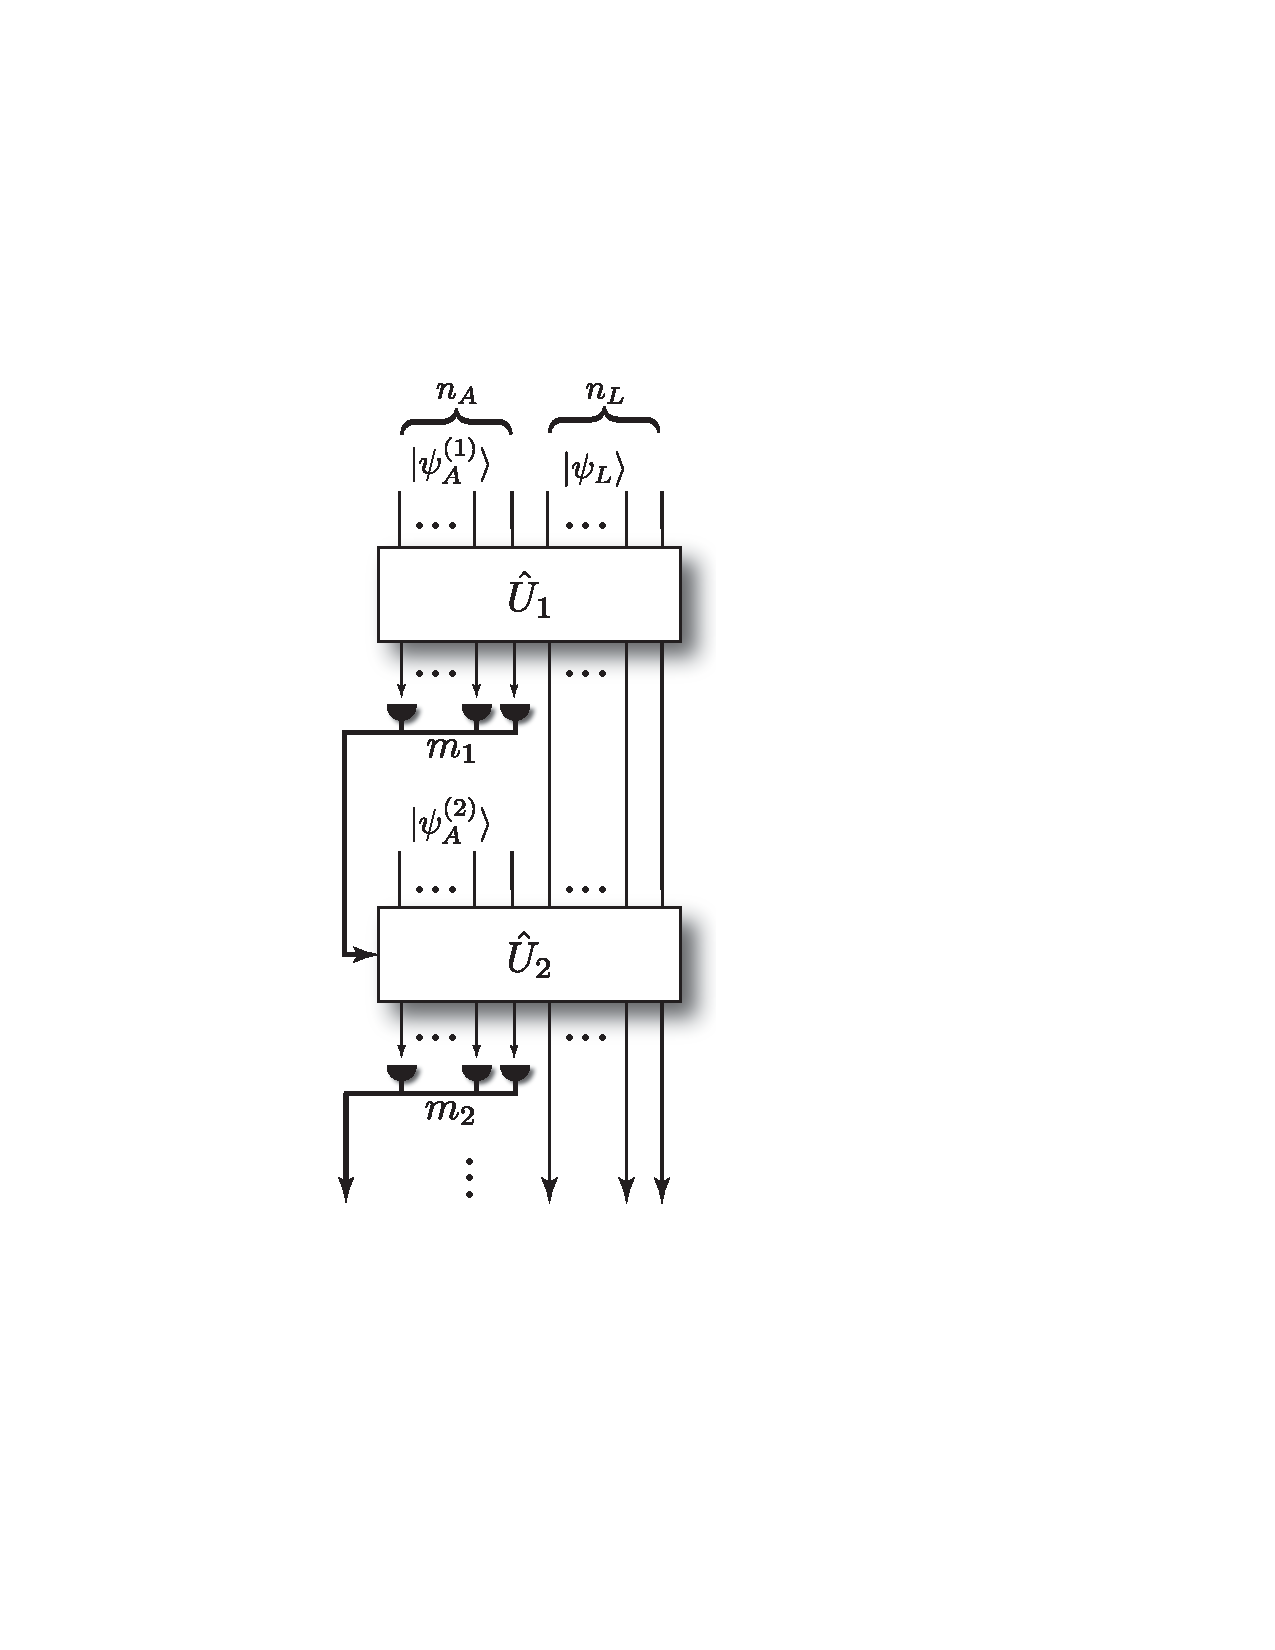
\includegraphics[width=0.5\columnwidth]{KLM}
\caption{KLM architecture for universal LOQC. $n_L$ optical modes are associated with logical qubits in the state $\ket{\psi_L}$, with the remaining $n_A$ modes acting as ancillary states, $\ket{\psi_A}$. A round of passive linear optics is applied, $\hat{U}_1$. Then the ancillary modes are measured, yielding some set of measurement outcomes $m_1$. These are classically processed to determine what the next round of passive linear optics, $\hat{U}_2$, ought to be. This repeats some polynomial number of times, from which an arbitrary quantum computation can be implemented. The {\sc BosonSampling} and quantum walk models are equivalent to taking just the first stage of this protocol: one round of input state, passive linear optics, and measurement.} \label{fig:KLM_protocol}
\end{figure}

Significant progress is being made on reconfigurable, integrated LOQC devices \cite{bib:UniversalLOOBrien}, but switching times remain orders of magnitude slower than required for fast-feedforward. The resource overhead associated with overcoming the non-determinism of entangling gates is substantial in the original KLM proposal. But despite being improved upon by orders of magnitude using cluster state approaches \cite{bib:Nielsen04, bib:BrowneRudolph05}, resource scaling remains daunting. It therefore seems most likely that certain elements from LOQC might be combined into hybrid architectures, to be discussed in detail in Sec.~\ref{sec:hybrid}.

\subsubsection{Passive Linear Optics} \label{sec:BS}

While the KLM protocol is universal for quantum computing, some of the key technological requirements are very challenging, and unlikely to be achieved in the short-term. However, simplified yet non-universal models for optical quantum computing can abandon some of the more challenging requirements, nonetheless implementing a restricted set of post-classical quantum computations. The two main contenders are quantum walks \cite{bib:Aharonov93, bib:Aharonov01, bib:Kempe03, bib:Salvador12} and {\sc BosonSampling} \cite{bib:AaronsonArkhipov10, bib:RohdeIntroBS15}, both closely related in that they require only passive linear optics and single-photon states. Since, evidence has been presented that similar passive linear optics protocols may implement computationally hard problems using states of light other than photon-number states \cite{bib:RandBS, bib:RohdePhotAdd15, bib:RohdeDisp15, bib:RohdeCat15}.

These protocols involve nothing more than evolving single-photon states through beamsplitter networks and measuring the output photostatistics. This is equivalent to just taking the first stage of the KLM protocol shown in Fig.~\ref{fig:KLM_protocol}. The computational hardness of these models for computation relate to the fact that the amplitudes in the output superpositions are related to matrix permanents, which are \textbf{\#P}-hard in general, yielding computationally complex sampling problems.

Both quantum walks and {\sc BosonSampling} have been subject to extensive experimental investigation in recent years \cite{bib:PeruzzoQW, bib:Broome10, bib:Schreiber11b, bib:Owens11, bib:RohdeQWExp12, bib:Broome2012, bib:RohdeQWExp12, bib:Spring2, bib:Crespi3, bib:Tillmann4}.

Because these models are entirely passive, they can be made cloud-based very trivially: Alice prepares her permutation of single photons as the input state, sends it to Bob over the quantum network, who applies the passive operations before returning the state to Alice. Importantly, no intermediate client/server interaction is required. Alternately, she could classically communicate a bit-string to Bob indicating the input photon-number configuration, in case she is unable to prepare it herself.

It was recently shown that this model may be trivially homomorphically encrypted with the addition of additional photons and randomised polarisation rotations on the inputs \cite{bib:RohdeQWEnc12}. This encryption also does not require any client/server interaction, remaining completely passive, yet achieving near optimal secrecy.

\subsubsection{Continuous Variables}

\comment{TO DO}

Sec.~\ref{sec:CV_enc}
\cite{bib:Menicucci06, lund, ralph, weedbrook}
Cat states
Gaussian states

\subsubsection{Hybrid Architectures} \label{sec:hybrid}

It is unlikely that future, large-scale quantum computers will be purely optical. Some other technologies have a more favourable outlook in terms of scalability. Nonetheless, when it comes to networking quantum computers, optics is the natural approach, motivating investigation of hybrid architectures, where qubits are represented using some non-optical system, but entangling operations between them are mediated by optical states. The natural example is qubits which couple to single-photon states, whereupon which-path erasure between coupled optical modes teleports entanglement onto the physical qubits. Similarly, measurement of the qubits is performed by stimulating the emission of photons from the physical qubits. This idea has been applied to $\lambda$-configuration atomic qubits \cite{bib:BarrettKok05}, shown in Fig.~\ref{fig:barrett_kok}, and atomic ensemble qubits \cite{bib:RohdeAtEns10}.

\begin{figure}[!htb]
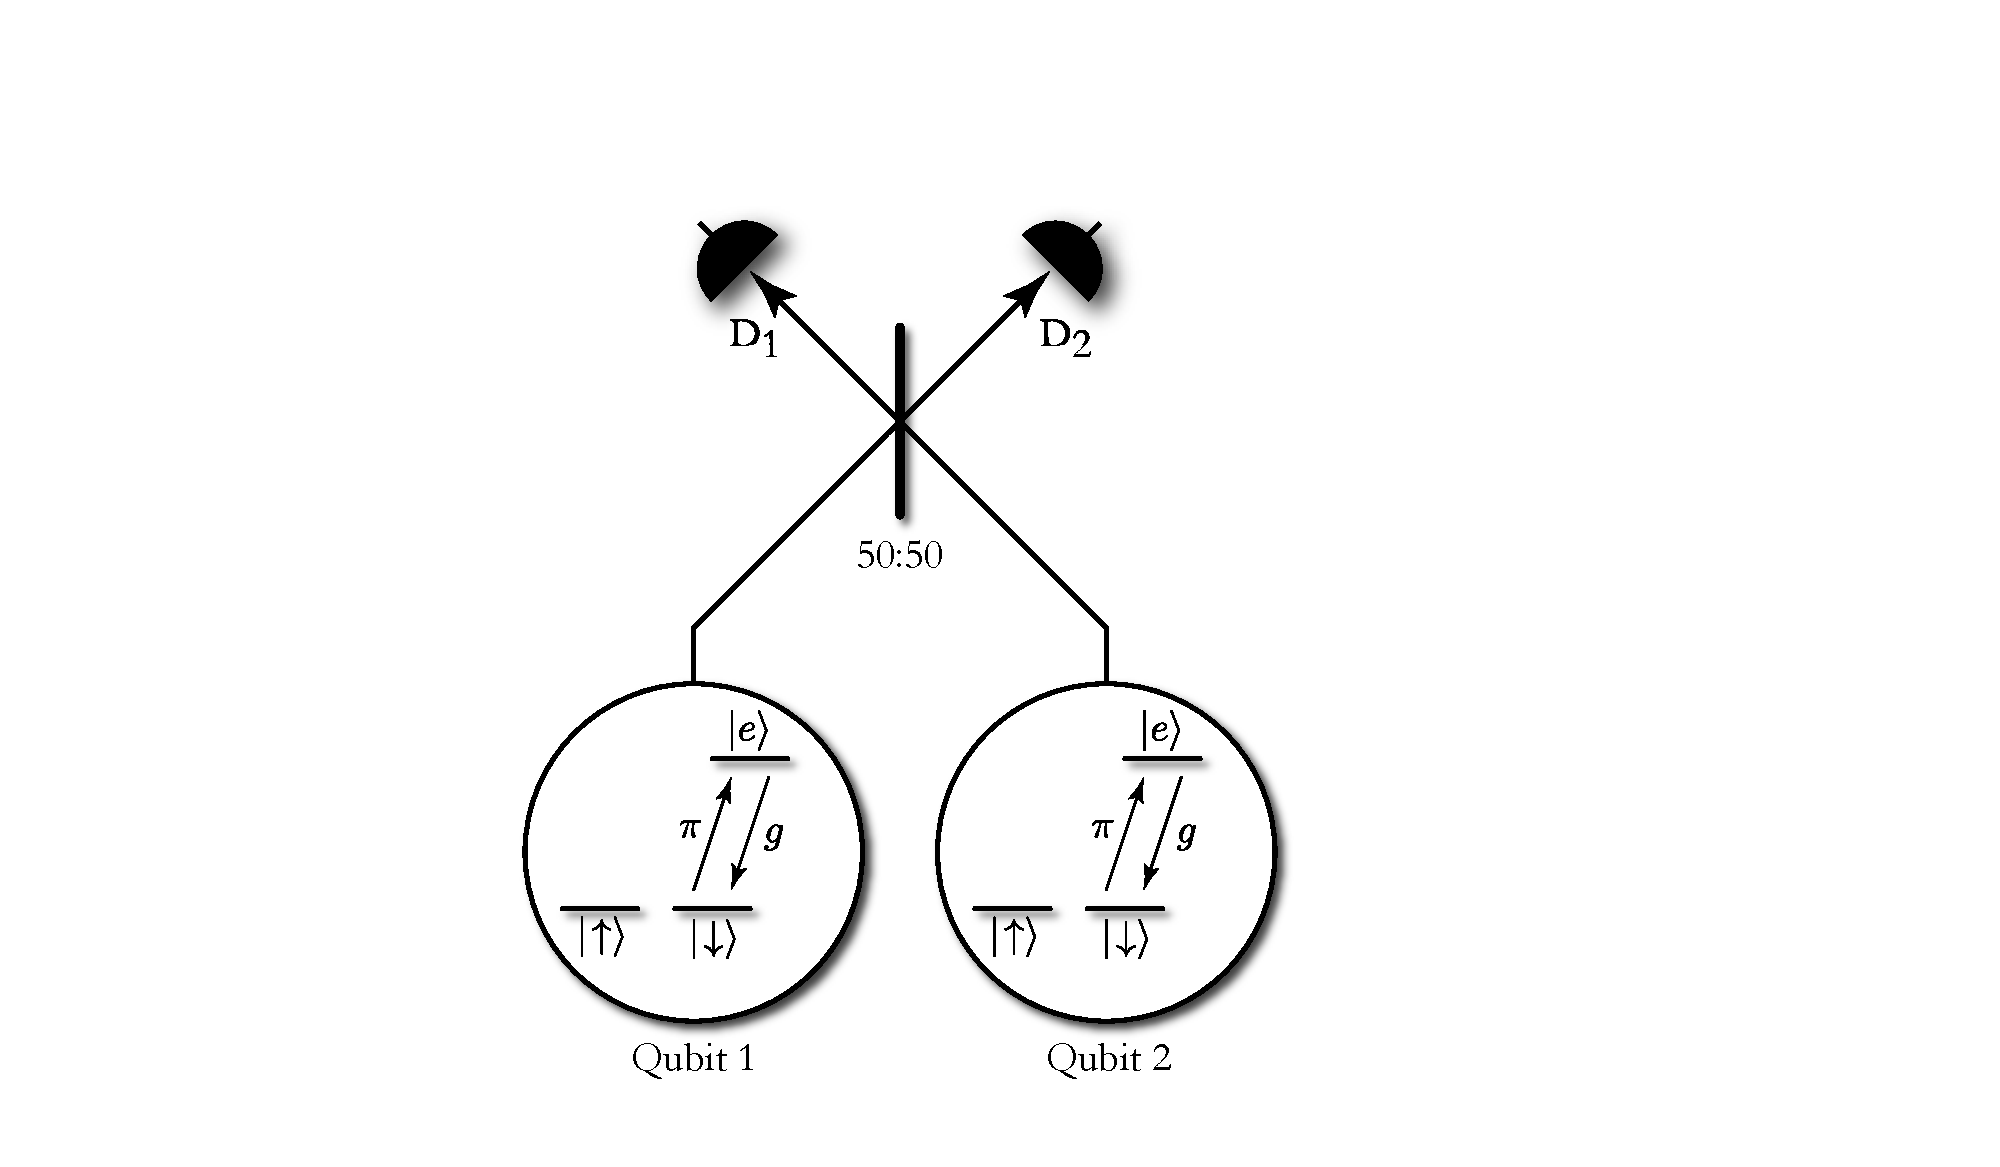
\includegraphics[width=0.75\columnwidth]{barrett_kok}
\caption{Two atomic systems in $\lambda$-configurations, each coupled with an optical mode. An entangling operation between them is mediated via linear optics \cite{bib:BarrettKok05}. Each system contains two ground states, which jointly encode a qubit ($\ket{\!\uparrow}$, $\ket{\!\downarrow}$), and an additional excited state ($\ket{e}$), which only couples to the $\ket{\!\downarrow}$ state. A $\pi$-pulse excites the electron from the $\ket{\!\downarrow}$ to the $\ket{e}$ state, after which emission of a photon is associated with a relaxation back to $\ket{\!\downarrow}$. If the two optical modes are interfered on a 50:50 beamsplitter, and a single photon is detected between the two photodetectors, $D_1$ and $D_2$, which-path erasure entangles the two qubits into a maximally entangled Bell pair. More complicated networks based on this entangling operation allow the preparation of cluster states, enabling universal quantum computation. In a quantum networking context, the matter qubits could be held by a client, and the optical interferometry implementing the computation outsourced to the cloud, i.e $D_1$ and $D_2$ are routed into the quantum network.} \label{fig:barrett_kok}
\end{figure}

The attractive feature of this type of approach is that the actual entanglement is generated using all-optical operations, despite the underlying logical qubits being stationary. This allows the entangling operations to be performed remotely in the cloud, without moving the qubits. Such hybrid systems present an interesting platform for cloud quantum computing -- despite the qubits being stationary, we are able to outsource the interactions between them to distant servers.

More generally, we can envisage that future quantum networks interfacing with arbitrary physical architectures for quantum computing will require \emph{interfaces}, coupling the quantum states of different types of physical systems for representing qubits. This is an area of research under active development \cite{???}, and will be instrumental in the development of the quantum internet. For example, much progress has been made in coupling photonic qubits with atomic \cite{???}, quantum dot \cite{???}, and atomic ensemble \cite{???} systems, with rapidly improving coupling efficiencies and fidelities.

\subsubsection{Modularised Computation}

How does one build a large-scale quantum computer, given the extremely daunting technological requirements. In any industry, economies of scale allow the mass production, and rapid decrease in the price of technology. To achieve this, we must find a way to make quantum technologies commodity items, which avoid all the hassle of cutting-edge labs.

In Sec.~\ref{sec:dist_QC} we introduced the notion of distributed quantum computation. There the motivation was to enable a computation to be distributed across multiple servers, which either parallelise computation or process it as a pipeline in series.

An alternate direction, for economic reasons, is that it is unviable for a single server to host an entire computation. Rather, hosts will have limited capability, and to perform a large-scale computation will require employing a potentially large number of hosts cooperating with one another. This can be regarded as the most general incarnation of distributed computation.

This is not the same motivation as for in-series computation, where different servers in the pipeline have different proprietary algorithms as subroutines of a larger computation. And it also differs from in-parallel computation, where multiple servers implement the same algorithm on different data, which is subsequently merged by a root node, as per, for example, a {\sc MapReduce}-style protocol.

Instead, the motivation is one of economics -- individual servers will have finite resources, but there may be many of them, which can be networked to implement a larger algorithm virtually.

The concept of this model is best explained using the cluster state formalism (Sec.~\ref{sec:CSQC}), which lends itself naturally to this approach.

A rectangular lattice graph is sufficient for universal quantum computation, even if the cluster state graph is not local (but classical communication between nodes is allowed).

Let us first assume that we wish to construct a cluster state with $n_\mathrm{logical}$ logical qubits. We additionally allow each logical qubit to be the root node of a graph with a $+$ structure, where each branch comprises $n_\mathrm{ancilla}$ ancillary physical qubits. These collectively form a single \emph{module} in the topology. Our goal is to fuse modules via nearest neighbour entanglement.

There are several identities that we will shortly make use of, which we will introduce here. First, a measurement of any qubit in the $\hat{Z}$ basis removes that vertex from the graph, and any edges emanating from the removed vertex. Second, the measurement of a qubit in the $\hat{Y}$ basis removes that qubit, and creates links between all its neighbours. Finally, upon success, a CZ gate creates a new edge between the two qubits acted upon by the gate. In the event of failure (since the gate is non-determinisitic), both qubits acted upon by the gate are effectively measured in the $\hat{Z}$ basis, i.e they, and associated edges, are removed from the graph, thereby shortening the respective branches. This is summarised in Fig.~\ref{fig:cluster_ident}.

\begin{figure}[!htb]
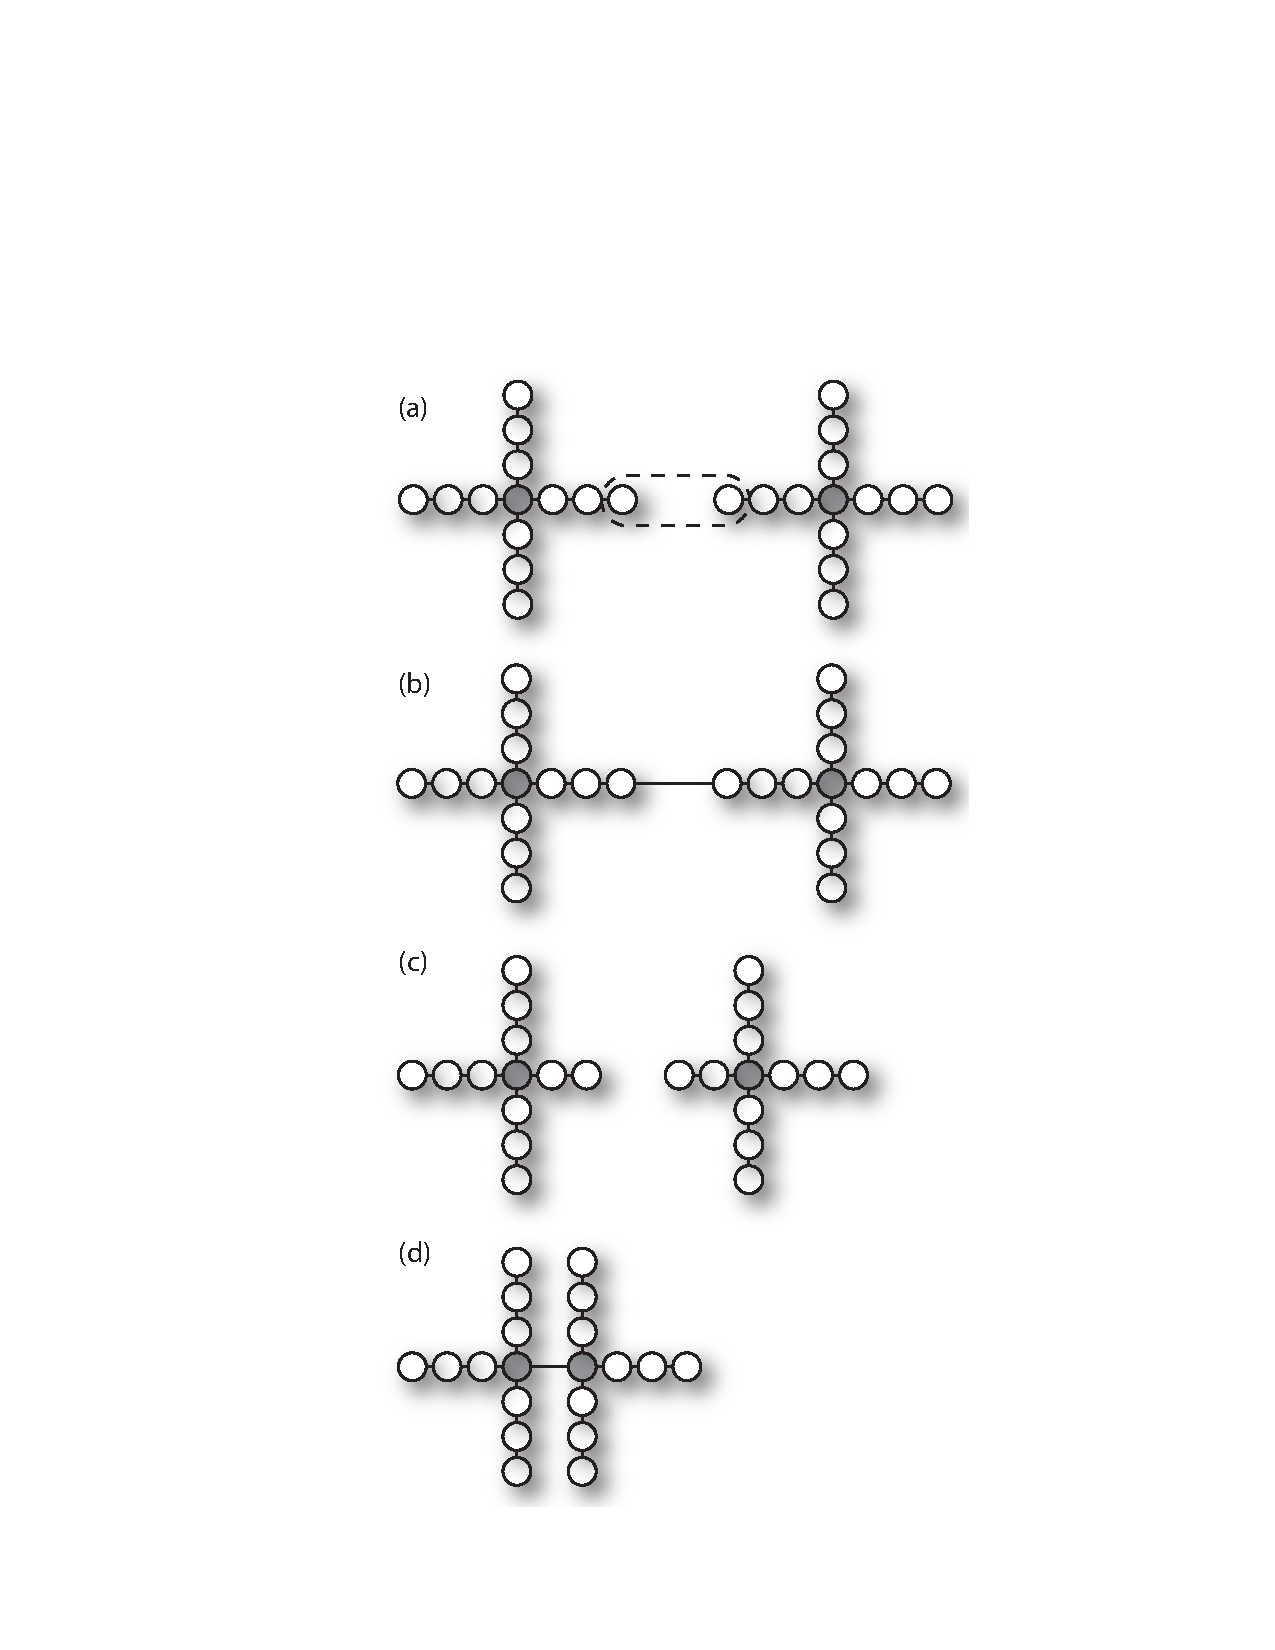
\includegraphics[width=\columnwidth]{cluster_ident}
\caption{Several cluster state identities. (a) Two cluster states with a $+$ topology are fused together using an EO (dashed). (b) Upon success, an edge is created between the respective qubits. (c) Upon failure, both qubits are effectively measured in the $\hat{Z}$ basis, thereby removing them, and any associated edges, from the graph. (d) Following a successful EO, the unwanted ancillary qubits may be eliminated using measurements in the $\hat{Y}$ basis, creating edges between their neighbours. If the grey qubits represent the desired logical qubits, this can be used to remove the remainder of the branches emanating from them.} \label{fig:cluster_ident}
\end{figure}

We arrange the modules to internally represent a $+$ topology where each node has neighbouring branches in each of the up/down/left/right directions. But we imagine the situation whereby each logical qubit, along with its respective ancillary branches, is held by a different server. Thus, the final cluster state is truly decentralised across all the servers, and in general local computations cannot be performed.

Using the ancillary states in the respective directions, we attempt to fuse neighbouring clusters using entangling operations (EO's), such as CZ gates (e.g a KLM CZ gate), linear optics \emph{fusion gates} (i.e rotated polarising beamsplitters) \cite{???}, or atoms with a $\lambda$-configuration coupled to photons \cite{barrett}. Importantly, using the fusion gate approach, only a single beamsplitter is required to perform the EO, which only necessitates high-visibility HOM \cite{HOM} interference, mitigating the need for far more challenging interferometric stability.

When an EO is successful, we have fused two logical qubits together, albeit potentially with ancillary states between them. When it fails, we have lost the respective ancillary states, and we attempt again using the next ancillary qubits in each of the the respective branches. The bonding only fails if all $n_\mathrm{ancilla}$ EO's fail. Upon successful bonding, any remaining ancillary qubits between the respective logical qubits are measured in the $\hat{Y}$ basis to remove the intermittent ancillary qubits, whilst connecting their neighbours, leaving the two respective logical qubits as nearest neighbours in the graph. Our goal is for the entire graph to have a lattice structure, once ancillary qubits have been measured out. These ideas are illustrated in Fig.~\ref{fig:module}.

\begin{figure}[!htb]
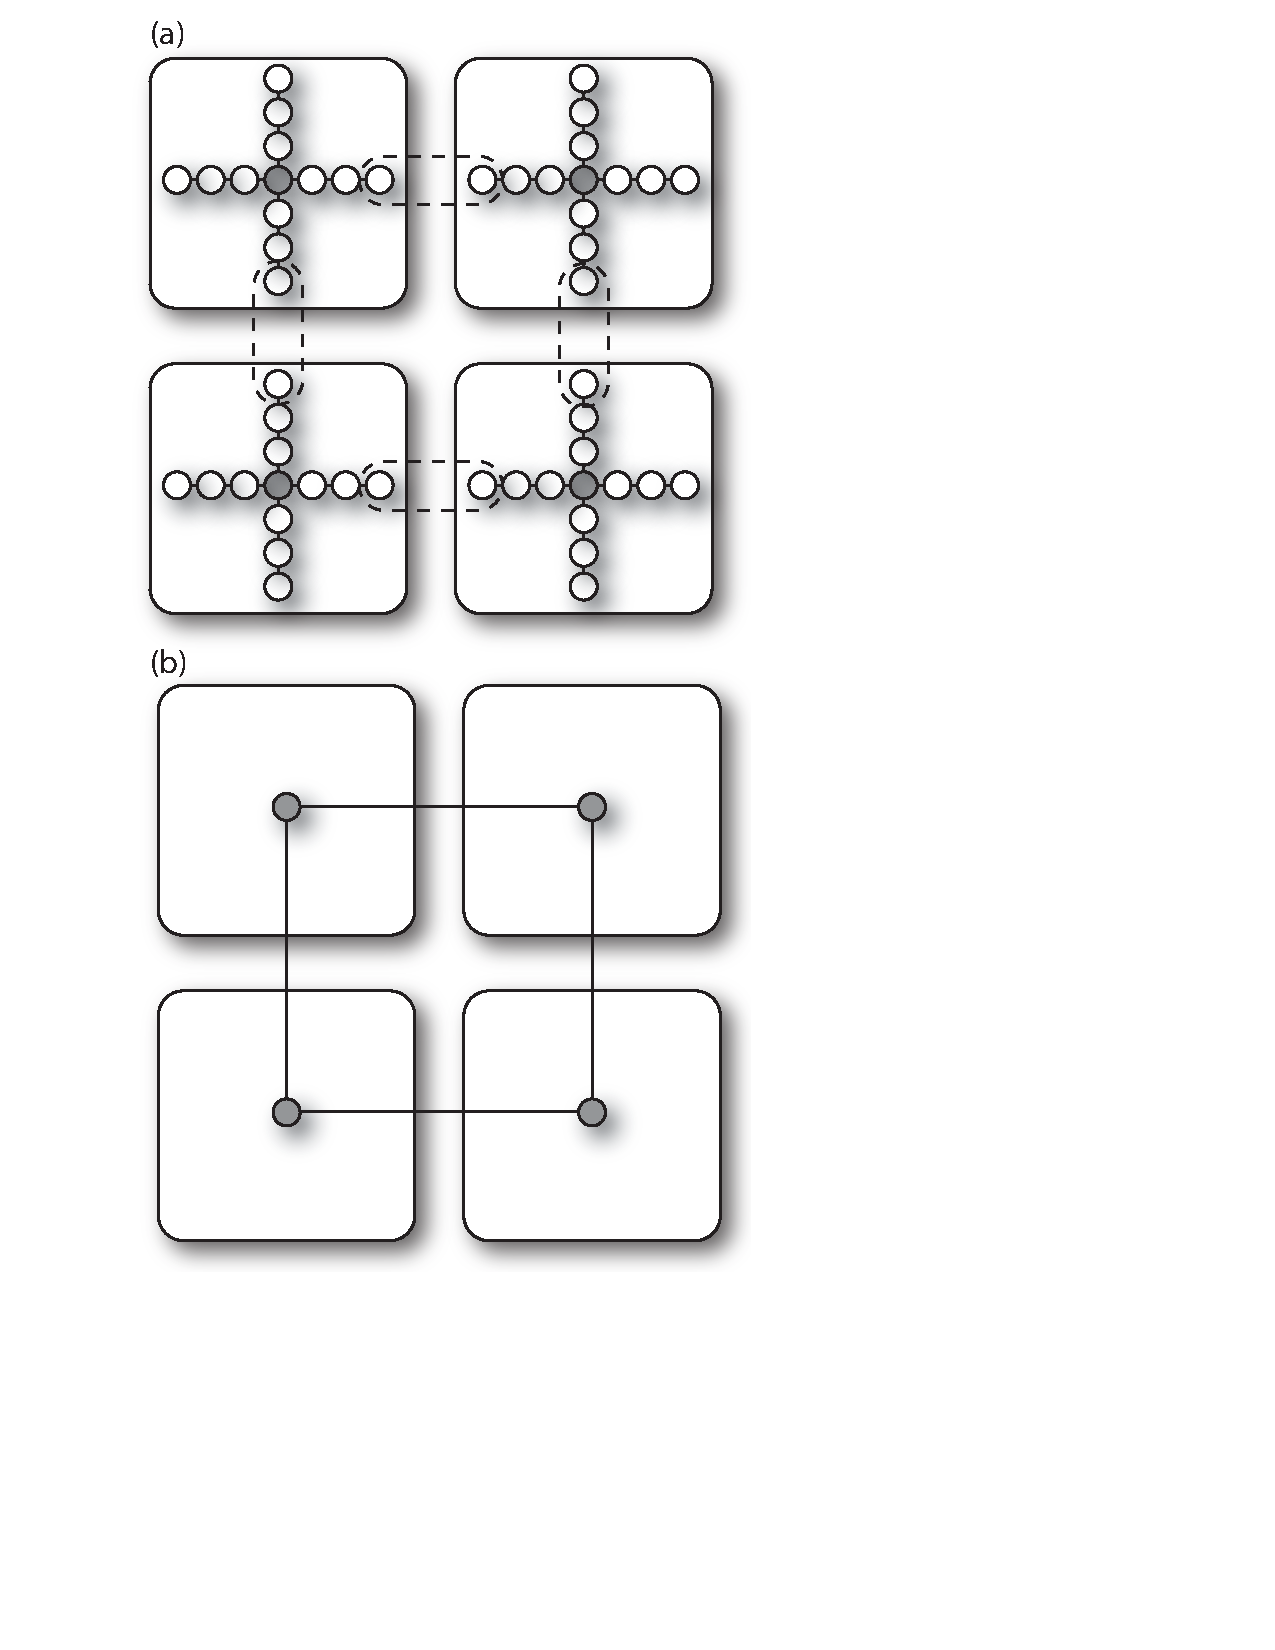
\includegraphics[width=\columnwidth]{module}
\caption{The modularised approach to scalable and economically efficient, distributed quantum computation using cluster states. We consider a simple \mbox{$2\times 2$} case where each module (rounded rectangles) comprises a single logical qubit (centre of each module in grey) and a number of ancillary qubits (white in each module), which facilitate bonding the logical qubits of nearest neighbours. The preparation of the modules is performed via nearest neighbour EO's, beginning at the end of branches, and working towards the root node upon each failure, until (hopefully) an EO is successful.} \label{fig:module}
\end{figure}

The probability of successfully creating an edge between two logical qubits is then,
\begin{align}
p_\mathrm{success} = 1 - {p_\mathrm{failure}}^{n_\mathrm{ancilla}},
\end{align}
and the probability of preparing the entire lattice (ignoring boundary conditions for simplicity) is,
\begin{align}
p_\mathrm{total} = O({p_\mathrm{success}}^{n_\mathrm{logical}}).
\end{align}
The number of logical qubits that may be prepared in the final lattice is therefore,
\begin{align}
n_\mathrm{logical} &= \frac{\mathrm{log}(p_\mathrm{total})}{\mathrm{log}(p_\mathrm{success})} \nonumber \\
&= \frac{\mathrm{log}(p_\mathrm{total})}{\mathrm{log}(1 - {p_\mathrm{failure}}^{n_\mathrm{ancilla}})} \nonumber \\
&= \mathrm{log}({p_\mathrm{failure}}^{n_\mathrm{ancilla}} + p_\mathrm{total} - 1) \nonumber \\
&= O(n_\mathrm{ancilla}).
\end{align}
Thus, we have efficient (linear) scaling in the number of required ancillary qubits against the desired number of logical qubits. This implies that when distributing a computation using this approach, the resource overhead is efficient.
\comment{Check this!}

Of course, this is the most simple model, with a single logical qubit per module. In due course, we would expect modules to become far more capable.

\section{State of the Art}

\comment{TO DO! Talk about where different technologies are currently at. What are some realistic cost metrics etc. What protocols have been demonstrated? What's coming in the near future?}

\section{The Economics of the Quantum Internet} \label{sec:economics}

Quantum computers are highly likely to, at least initially, be extremely expensive, and affordable outright by few. Thus, client/server economic models based on outsourcing of computations to servers on a network, will be essential to making quantum computing widely accessible. The protocols we have presented here pave the way for this type of economic model to emerge. It is paramount that the types of technologies introduced here be fully developed in time for the deployment of useful quantum computing hardware, such that they can be fully commercialised from day one of their availability, enabling widespread adoption, enhanced economy of scale, and rapid proliferation.

A key question regarding the economics of the quantum internet is the extent to which it will be able to piggyback off existing optical communications infrastructure, given that networking will almost inevitably be optically mediated. We have an existing intercontinental fibre-optic backbone, as well as sophisticated satellite networks. To what extent will this existing infrastructure (or future telecom infrastructure) be able to be exploited so as to avoid having to rebuild the entire future quantum internet infrastructure from scratch? This is a question worth tens of billions of dollars. We also need to factor in that given the massive driving force behind telecom technology, its cost is following a Moore's Law-like trajectory, and what costs a billion dollars today might cost a million dollars in a decade's time. In light of this, telecom wavelength quantum optics is being hotly pursued \cite{???}. And at the time of writing this paragraph, a world-leading Chinese experimental team has just successfully launched a QKD satellite into low Earth orbit, enabling intercontinental QKD, with talk of the next space race being the one for quantum supremacy.

Technology should benefit humanity, not only an elite few. In light of this, who exactly will benefit from the quantum internet? Its beauty is that it doesn't create a system of winners and losers. Rather, it establishes a technological infrastructure from which all can benefit, rich or poor. Well-resourced operators who can afford quantum computers, for example, will benefit from being able to license out compute time on their computers, ensuring no wasted clock-cycles and maximising efficiency. The less-well-resourced will benefit in that they will have a means by which to access the extraordinary power of quantum computing on a licensed basis, facilitating access to infrastructure by those who otherwise would have been priced out of the market. This is essentially the same model as what is employed by some present-day supercomputer operators, enabling small players access to supercomputing infrastructure. The quantum internet is critical to achieving the same goal. This could have transformative effects on the developing world in particular.

The quantum internet will facilitate the communication and trade of quantum assets beyond just quantum computation and cryptography. There are many uses for various hard-to-prepare quantum states, for example in metrology or lithography, where outsourcing state preparation would be valuable. Alternately, performing some quantum measurements can be technologically challenging, and the ability to delegate them to someone better-equipped would be desirable. The quantum internet goes beyond just quantum computing. Rather, it extends to a full range of quantum resources.

To commodify quantum computing, if constructing large-scale quantum computers were a simple matter of plug-and-play, where quantum Lego building blocks are available off-the-shelf and straightforward to assemble even for monkeys, mass-production would rapidly force down prices. By arbitrarily interconnecting these boxes, large-scale quantum computers could be scaled up with demand.

We envisage that each of these commodity items is a black box, within which a relatively small number of qubits are present. Then, to build a larger quantum computer, we don't need to upgrade our boxes. Rather, we simply purchase more boxes to connect to the network. Following this model, these black boxes would become mass-produced commodity items, allowing quantum computers of arbitrary size to be economically scaled up, and broadly accessible as mass-production drives down costs. This notion is tailored to cluster states in particular -- because a cluster state can be obtained by nearest neighbour interactions, and all preparation stages commute with one another, they naturally lend themselves to distributed preparation.

On the other hand, if quantum computers were only ever sold as room-sized, complete solutions (think D-Wave), such mass-production would not experience the driving force of commodified, off-the-shelf building blocks, each of which is cheap, yet frugal in its computational power alone.

Modularised quantum computation mitigates the need to purchase large-scale quantum computers outright, allowing them to be gradually scaled up as demand increases and production costs diminish.

While the power of classical computers scales roughly linearly with the number of transistors, the power of quantum computers scales exponentially with the number of qubits. The classical Moore's law is close to saturation -- we simply can't make transistors too much smaller than they already are! We therefore envisage a new quantum Moore's law, which follows a far more impressive trajectory than its classical counterpart. The point of critical mass in quantum computing will take place when the classical and quantum Moore's law extrapolations intersect, signalling the commencement of the post-classical era. A somewhat speculative trend for this kind of scaling is illustrated in Fig.~\ref{fig:moores}, based on current real-world data and making plausible extrapolations thereof.

\begin{figure}[!htb]
%includegraphics[width=\columnwidth]{module}
\caption{Superimposed are Moore's law for the power of classical computers (bottom), with a speculated quantum version of Moore's law (top). The point of intersection signals the beginning of the post-classical era for quantum computing. The somewhat speculative curves suggest that this era might arrive already in the not too distant future.} \label{fig:moores}
\end{figure}

\section{The Vision of the Global Quantum Internet}

Quantum technologies, particularly quantum computing, will truly revolutionise countless industries. With early demonstrations of key quantum technologies -- such as QKD, long distance quantum teleportation, and quantum computing -- becoming a reality, it is of utmost importance that networking protocols be pursued.

We have presented an early formulation and analysis of quantum networking protocols with the vision of enabling a future quantum internet, where quantum resources can be shared and communicated in much the same way as is presently done with digital assets. Whilst it is hard to foresee exactly how future quantum networks will be implemented, many of the central ideas presented here will be applicable across architectures and implementations on an ad hoc basis.

There are a number of schools of thought one might subscribe to when quantum networking. One might demand perfect data integrity and best-case network performance. But that would come at the expense of necessitating an all-powerful central authority to oversee all communications and ensure that scheduling was absolutely perfect -- a potentially very challenging optimisation problem. Or one might tolerate lost data packets or suboptimal performance, but at the expense of limiting the applicability of the network. Or maybe some arbitrary compromise between different metrics and attributes is best. These are open questions that needn't have concrete, one-size-fits-all answers. The QTCP framework we presented is sufficiently flexible and extensible that these questions can be answered and enforced independently by different subnetworks, depending on their individual characteristics and requirements, in much the same way that every organisation connected to the classical internet today is free to structure their own LAN as they please, enforcing their own network policies.

The quantum internet will allow quantum computation to become distributed, not just outsourced. In the same way that many present-day classical algorithms are heavily parallelised and distributed across large clusters, or even across the internet itself (e.g the SETI project), quantum networks will allow the distribution of quantum computation across many nodes, either in parallel, in series, or in a modulerised fashion. This will be central to achieving scalability. Keeping in mind that the classical-equivalent power of a quantum computer grows exponentially with the number of qubits, it is highly desirable to squeeze out every last available qubit for our computations.

Combined with recent advances in homomorphic encryption and blind quantum computation, commercial models for the distribution of quantum computation will emerge, allowing computational power to be outsourced, with both client and server confident in the security of their data and proprietary algorithms. This is a notion that is challenging on classical computers, but will be of utmost importance in quantum computing, where it is expected sensitive data and algorithms will often be at stake.

From the security perspective, the global quantum internet will enable an international QKD communications network with perfect secrecy, guaranteed by the laws of physics. This will be of immense economic and strategic benefit to commercial enterprises, governments, and individuals. Classical cryptography is already a multi-billion dollar industry worldwide. Quantum cryptography will supersede it, and be of especial importance in the era of quantum computers, which compromise some essential classical cryptographic protocols, such as RSA \cite{bib:RSA}, which forms the basis of most current internet encryption. Not only is quantum cryptography being pursued optically, but even credit cards with embedded quantum circuitry are being actively developed to prevent fraud. Inevitably, this will require the communication between bank automats and servers to be mediated by a quantum network.

The reality is that we are only just beginning to understand the full potential for quantum technologies, and as we learn more we will inevitably find new uses for networking them.

Large-scale quantum computing may still seem a formidable, and somewhat long-term challenge. But it isn't likely to remain so. Once we have mastered the technological art of preparing qubits and implementing high-fidelity entangling operations between them, it is just a matter of sitting back and watching Gordon Moore perform his witchcraft, and scalability of quantum technology, and its rapid market-driven reduction in cost, will quickly ensue. The quantum internet will drive this rapid development by expanding the demand for access to this technology.

It is essential for the adoption of quantum technology, that quantum networking infrastructure be sufficiently well developed that it is ready to be deployed the minute the first useful, post-classical hardware becomes available. The proliferation of the defining technology of the 21st century depends upon it.

\emph{--- Ad astra per alas fideles. Scientia potentia est.}

\begin{acknowledgments}
P.P.R. thanks Neil Dawson, David Aldred, Ben Laybutt, Tess Moffat, Sophie Marrio, James Sudburry, Ruina Wang and Charlotte Bridault for tolerating him during this project.
\end{acknowledgments}

\bibliography{quantum_internet}

\end{document} 